% Options for packages loaded elsewhere
% Options for packages loaded elsewhere
\PassOptionsToPackage{unicode}{hyperref}
\PassOptionsToPackage{hyphens}{url}
\PassOptionsToPackage{dvipsnames,svgnames,x11names}{xcolor}
%
\documentclass[
  spanish,
  10pt,
]{article}
\usepackage{xcolor}
\usepackage{amsmath,amssymb}
\setcounter{secnumdepth}{5}
\usepackage{iftex}
\ifPDFTeX
  \usepackage[T1]{fontenc}
  \usepackage[utf8]{inputenc}
  \usepackage{textcomp} % provide euro and other symbols
\else % if luatex or xetex
  \usepackage{unicode-math} % this also loads fontspec
  \defaultfontfeatures{Scale=MatchLowercase}
  \defaultfontfeatures[\rmfamily]{Ligatures=TeX,Scale=1}
\fi
\usepackage{lmodern}
\ifPDFTeX\else
  % xetex/luatex font selection
  \setmainfont[]{Arial}
\fi
% Use upquote if available, for straight quotes in verbatim environments
\IfFileExists{upquote.sty}{\usepackage{upquote}}{}
\IfFileExists{microtype.sty}{% use microtype if available
  \usepackage[]{microtype}
  \UseMicrotypeSet[protrusion]{basicmath} % disable protrusion for tt fonts
}{}
\makeatletter
\@ifundefined{KOMAClassName}{% if non-KOMA class
  \IfFileExists{parskip.sty}{%
    \usepackage{parskip}
  }{% else
    \setlength{\parindent}{0pt}
    \setlength{\parskip}{6pt plus 2pt minus 1pt}}
}{% if KOMA class
  \KOMAoptions{parskip=half}}
\makeatother
% Make \paragraph and \subparagraph free-standing
\makeatletter
\ifx\paragraph\undefined\else
  \let\oldparagraph\paragraph
  \renewcommand{\paragraph}{
    \@ifstar
      \xxxParagraphStar
      \xxxParagraphNoStar
  }
  \newcommand{\xxxParagraphStar}[1]{\oldparagraph*{#1}\mbox{}}
  \newcommand{\xxxParagraphNoStar}[1]{\oldparagraph{#1}\mbox{}}
\fi
\ifx\subparagraph\undefined\else
  \let\oldsubparagraph\subparagraph
  \renewcommand{\subparagraph}{
    \@ifstar
      \xxxSubParagraphStar
      \xxxSubParagraphNoStar
  }
  \newcommand{\xxxSubParagraphStar}[1]{\oldsubparagraph*{#1}\mbox{}}
  \newcommand{\xxxSubParagraphNoStar}[1]{\oldsubparagraph{#1}\mbox{}}
\fi
\makeatother


\usepackage{longtable,booktabs,array}
\usepackage{calc} % for calculating minipage widths
% Correct order of tables after \paragraph or \subparagraph
\usepackage{etoolbox}
\makeatletter
\patchcmd\longtable{\par}{\if@noskipsec\mbox{}\fi\par}{}{}
\makeatother
% Allow footnotes in longtable head/foot
\IfFileExists{footnotehyper.sty}{\usepackage{footnotehyper}}{\usepackage{footnote}}
\makesavenoteenv{longtable}
\usepackage{graphicx}
\makeatletter
\newsavebox\pandoc@box
\newcommand*\pandocbounded[1]{% scales image to fit in text height/width
  \sbox\pandoc@box{#1}%
  \Gscale@div\@tempa{\textheight}{\dimexpr\ht\pandoc@box+\dp\pandoc@box\relax}%
  \Gscale@div\@tempb{\linewidth}{\wd\pandoc@box}%
  \ifdim\@tempb\p@<\@tempa\p@\let\@tempa\@tempb\fi% select the smaller of both
  \ifdim\@tempa\p@<\p@\scalebox{\@tempa}{\usebox\pandoc@box}%
  \else\usebox{\pandoc@box}%
  \fi%
}
% Set default figure placement to htbp
\def\fps@figure{htbp}
\makeatother


% definitions for citeproc citations
\NewDocumentCommand\citeproctext{}{}
\NewDocumentCommand\citeproc{mm}{%
  \begingroup\def\citeproctext{#2}\cite{#1}\endgroup}
\makeatletter
 % allow citations to break across lines
 \let\@cite@ofmt\@firstofone
 % avoid brackets around text for \cite:
 \def\@biblabel#1{}
 \def\@cite#1#2{{#1\if@tempswa , #2\fi}}
\makeatother
\newlength{\cslhangindent}
\setlength{\cslhangindent}{1.5em}
\newlength{\csllabelwidth}
\setlength{\csllabelwidth}{3em}
\newenvironment{CSLReferences}[2] % #1 hanging-indent, #2 entry-spacing
 {\begin{list}{}{%
  \setlength{\itemindent}{0pt}
  \setlength{\leftmargin}{0pt}
  \setlength{\parsep}{0pt}
  % turn on hanging indent if param 1 is 1
  \ifodd #1
   \setlength{\leftmargin}{\cslhangindent}
   \setlength{\itemindent}{-1\cslhangindent}
  \fi
  % set entry spacing
  \setlength{\itemsep}{#2\baselineskip}}}
 {\end{list}}
\usepackage{calc}
\newcommand{\CSLBlock}[1]{\hfill\break\parbox[t]{\linewidth}{\strut\ignorespaces#1\strut}}
\newcommand{\CSLLeftMargin}[1]{\parbox[t]{\csllabelwidth}{\strut#1\strut}}
\newcommand{\CSLRightInline}[1]{\parbox[t]{\linewidth - \csllabelwidth}{\strut#1\strut}}
\newcommand{\CSLIndent}[1]{\hspace{\cslhangindent}#1}

\ifLuaTeX
\usepackage[bidi=basic]{babel}
\else
\usepackage[bidi=default]{babel}
\fi
\ifPDFTeX
\else
\babelfont{rm}[]{Arial}
\fi
% get rid of language-specific shorthands (see #6817):
\let\LanguageShortHands\languageshorthands
\def\languageshorthands#1{}


\setlength{\emergencystretch}{3em} % prevent overfull lines

\providecommand{\tightlist}{%
  \setlength{\itemsep}{0pt}\setlength{\parskip}{0pt}}



 


\usepackage{booktabs}
\usepackage{longtable}
\usepackage{array}
\usepackage{multirow}
\usepackage{wrapfig}
\usepackage{float}
\usepackage{colortbl}
\usepackage{pdflscape}
\usepackage{tabu}
\usepackage{threeparttable}
\usepackage{threeparttablex}
\usepackage[normalem]{ulem}
\usepackage{makecell}
\usepackage{xcolor}
% Paquetes necesarios
\usepackage{amsmath}
\usepackage{amssymb}
\usepackage{graphicx}
\usepackage{fancyhdr}
\usepackage{geometry}
\usepackage{booktabs}
\usepackage{dcolumn}
\usepackage{array}
\newcolumntype{d}[1]{D{.}{.}{#1}}
\usepackage{float}
\usepackage{adjustbox}
% Paquete para controlar captions
\usepackage{caption}
% Fuente tiny para captions de figuras
\captionsetup[figure]{font=scriptsize}

% Configuración de márgenes
\geometry{
  a4paper,
  left=1.5cm,
  right=1.5cm,
  top=1.5cm,
  bottom=2.5cm,
  includeheadfoot
}

% Configuración de encabezado y pie de página
\pagestyle{fancy}
\fancyhf{} % Limpia encabezado y pie de página

% Encabezado
\lhead{
\includegraphics[height=1cm]{logo2.png}} % Logo en el encabezado
\chead{}
\rhead{\small Trabajo Final Neurociencias}

% Ajuste de separación entre encabezado y contenido
\setlength{\headheight}{2cm} % Altura del encabezado
\setlength{\headsep}{1.5cm} % Distancia entre encabezado y contenido

% Pie de página
\lfoot{}
\cfoot{\thepage} % Número de página centrado
\rfoot{}
\makeatletter
\@ifpackageloaded{caption}{}{\usepackage{caption}}
\AtBeginDocument{%
\ifdefined\contentsname
  \renewcommand*\contentsname{Tabla de contenidos}
\else
  \newcommand\contentsname{Tabla de contenidos}
\fi
\ifdefined\listfigurename
  \renewcommand*\listfigurename{Listado de Figuras}
\else
  \newcommand\listfigurename{Listado de Figuras}
\fi
\ifdefined\listtablename
  \renewcommand*\listtablename{Listado de Tablas}
\else
  \newcommand\listtablename{Listado de Tablas}
\fi
\ifdefined\figurename
  \renewcommand*\figurename{Figura}
\else
  \newcommand\figurename{Figura}
\fi
\ifdefined\tablename
  \renewcommand*\tablename{Tabla}
\else
  \newcommand\tablename{Tabla}
\fi
}
\@ifpackageloaded{float}{}{\usepackage{float}}
\floatstyle{ruled}
\@ifundefined{c@chapter}{\newfloat{codelisting}{h}{lop}}{\newfloat{codelisting}{h}{lop}[chapter]}
\floatname{codelisting}{Listado}
\newcommand*\listoflistings{\listof{codelisting}{Listado de Listados}}
\makeatother
\makeatletter
\makeatother
\makeatletter
\@ifpackageloaded{caption}{}{\usepackage{caption}}
\@ifpackageloaded{subcaption}{}{\usepackage{subcaption}}
\makeatother
\usepackage{bookmark}
\IfFileExists{xurl.sty}{\usepackage{xurl}}{} % add URL line breaks if available
\urlstyle{same}
\hypersetup{
  pdfauthor={Amaru Simón Agüero Jiménez},
  pdflang={es},
  colorlinks=true,
  linkcolor={blue},
  filecolor={Maroon},
  citecolor={Blue},
  urlcolor={Blue},
  pdfcreator={LaTeX via pandoc}}


\title{\begin{center}
  
\includegraphics[height=1.5cm]{logo2.png} \\[1cm]
  \Large Trabajo Final Neurociencias: \\ Estudio neurocomputacional del control cognitivo reactivo a través de paradigmas de Conflicto e Inhibición
\end{center}}
\author{Amaru Simón Agüero Jiménez}
\date{2025-07-22}
\begin{document}
\maketitle

\renewcommand*\contentsname{Tabla de contenidos}
{
\hypersetup{linkcolor=}
\setcounter{tocdepth}{3}
\tableofcontents
}

\newpage

\section{Introducción}\label{introducciuxf3n}

El control cognitivo se refiere al conjunto de procesos mentales de
orden superior que permiten un comportamiento flexible y dirigido a
objetivos, particularmente en presencia de información distractora o de
tendencias de respuestas pero inapropiadas\textsuperscript{1}. Estos
mecanismos son fundamentales para el comportamiento humano adaptativo,
permitiendo a los individuos anular impulsos automáticos, cambiar entre
tareas, actualizar información en la memoria de trabajo y resolver
conflictos. Dentro del amplio dominio del control cognitivo, dos
componentes son de importancia central para la investigación actual: el
monitoreo de conflictos y la inhibición de la
respuesta\textsuperscript{2}

El monitoreo y resolución de conflictos se refiere a la aptitud para
identificar la influencia de información no pertinente para la tarea,
así como para activar mecanismos de control con el fin de mitigarla,
garantizando de este modo que el comportamiento se mantenga en
consonancia con los objetivos establecidos\textsuperscript{3}. Este
proceso se estudia clásicamente utilizando paradigmas como la Tarea
Flanker de Eriksen, donde los participantes deben responder a un
objetivo central mientras ignoran información conflictiva de
distractores adyacentes, conocidos como flancos\textsuperscript{4} La
eficiencia de este sistema a menudo se indexa por el ``Efecto de
Compatibilidad Flanker'' (FCE, por sus siglas en inglés), donde las
respuestas son más lentas y menos precisas cuando los flancos son
incongruentes con el objetivo en comparación con cuando son
congruentes\textsuperscript{5,6}

La inhibición de la respuesta, por el contrario, es la capacidad de
suprimir o cancelar por completo una acción planificada o en
curso\textsuperscript{7}. Esta forma de control es crítica para
adaptarse a las demandas ambientales cambiantes y para reprimir
comportamientos socialmente inapropiados o contextualmente
incorrectos\textsuperscript{8}. La tarea Go/No-Go es un paradigma
canónico para evaluar la inhibición de la respuesta, requiriendo que los
participantes ejecuten una respuesta ``Go'' frecuente, pero que retengan
esta acción en ensayos ``No-Go'' infrecuentes\textsuperscript{9}. Los
fallos de inhibición en esta tarea, conocidos como ``falsas alarmas'',
proporcionan una medida directa de la capacidad de control inhibitorio
de un individuo\textsuperscript{10}.

La ejecución del control cognitivo no es monolítica; puede desplegarse
en al menos dos modos temporales distintos: control proactivo y
reactivo. El control proactivo implica el mantenimiento sostenido y
anticipatorio de información relevante para el objetivo para prepararse
para las próximas demandas cognitivas. Es un modo de control persistente
que sesga la atención y la selección de acciones por
adelantado\textsuperscript{11}. En contraste, el control reactivo es un
mecanismo transitorio, ``justo a tiempo'', que se recluta solo cuando se
detecta un evento de alto conflicto o una necesidad de inhibición. Las
manipulaciones experimentales que varían el tiempo disponible para la
preparación, como alterar el intervalo entre estímulos (ISI), pueden
cambiar sistemáticamente la dependencia de estos dos
modos\textsuperscript{12}. Los ISI más cortos (condiciones rápidas)
limitan la oportunidad de preparación proactiva, forzando una mayor
dependencia de mecanismos de control reactivo rápidos para manejar el
conflicto a medida que surge . El diseño experimental bajo
consideración, que incluye condiciones rápidas y lentas para las tareas
Flanker y Go/No-Go, está por lo tanto bien adaptado para investigar el
compromiso diferencial y la eficiencia de estos modos de
control\textsuperscript{13}.

\section{Análisis Exploratorio}\label{anuxe1lisis-exploratorio}

\subsection{La Tarea Flanker de Eriksen: Un Paradigma para la Resolución
de
Conflictos}\label{la-tarea-flanker-de-eriksen-un-paradigma-para-la-resoluciuxf3n-de-conflictos}

La Tarea Flanker de Eriksen representa uno de los paradigmas
experimentales más consolidados en el estudio del control cognitivo,
específicamente en la investigación de los mecanismos de resolución de
conflictos. En esta tarea, los participantes enfrentan el desafío de
identificar la dirección de una flecha central mientras simultáneamente
deben suprimir la información irrelevante proporcionada por flechas
flanqueadoras. La elegancia de este paradigma radica en su capacidad
para generar conflicto cognitivo de manera controlada y medible,
permitiendo así el estudio sistemático de los procesos de control
inhibitorio y atencional.

En la implementación actual del experimento, se emplearon cuatro
configuraciones de estímulos que varían sistemáticamente en su nivel de
conflicto. Los estímulos congruentes, representados por las
configuraciones \(>>>>>\) y \(<<<<<\), presentan flancos que apuntan en
la misma dirección que el objetivo central, facilitando así el
procesamiento y la respuesta. En contraste, los estímulos incongruentes,
manifestados en las configuraciones \(>><>>\) y \(<<><<\), introducen
información conflictiva al presentar flancos que apuntan en dirección
opuesta al objetivo, generando así la necesidad de un control cognitivo
aumentado para resolver el conflicto y producir la respuesta correcta.
Esta manipulación experimental se cruza factorialmente con una
manipulación de velocidad de respuesta, resultando en un diseño 2×2 que
permite examinar cómo la presión temporal modula los procesos de
resolución de conflictos.

La Figura 1 presenta la distribución fundamental de respuestas correctas
e incorrectas para cada patrón de flechas en ambas condiciones de
velocidad, revelando patrones que son consistentes con décadas de
investigación sobre el Efecto de Compatibilidad Flanker (FCE). En la
condición rápida (Figura 1A), emerge un patrón claro de deterioro del
rendimiento asociado con el conflicto. Los estímulos congruentes
muestran tasas de precisión notablemente altas, con el patrón \(>>>>>\)
alcanzando un 87.3\% de respuestas correctas (1,178 de 1,349 ensayos) y
el patrón \(<<<<<\) mostrando un rendimiento similar con 85.0\% de
precisión (1,176 de 1,384 ensayos). Esta alta precisión en los ensayos
congruentes contrasta marcadamente con el rendimiento en los ensayos
incongruentes, donde observamos una caída sustancial en la precisión. El
patrón \(>><>>\) produce solo un 73.6\% de respuestas correctas (944 de
1,282 ensayos), mientras que el patrón \(<<><<\) resulta en un 75.2\% de
precisión (988 de 1,314 ensayos).

El efecto de congruencia en la condición rápida puede cuantificarse
mediante la diferencia en las tasas de precisión promedio entre
condiciones:
\(\text{FCE}_{\text{precisión}} = \overline{P}_{\text{congruente}} - \overline{P}_{\text{incongruente}} = 86.15\% - 74.40\% = 11.75\%\).
Este efecto del 11.75\% representa una medida robusta de la
interferencia cognitiva generada por los flancos incongruentes bajo
presión temporal. Sin embargo, un hallazgo particularmente intrigante
emerge al examinar la condición lenta (Figura 1B). Aunque cabría esperar
que el tiempo adicional permitiera a los participantes resolver más
efectivamente el conflicto, observamos que el FCE no solo persiste sino
que se amplifica. En la condición lenta, los estímulos congruentes
alcanzan precisiones del 93.9\% y 95.4\%, mientras que los incongruentes
mantienen tasas de error considerables con precisiones del 75.5\% y
72.1\%. Esto resulta en un efecto de congruencia de
\(\text{FCE}_{\text{precisión-lenta}} = 94.65\% - 73.80\% = 20.85\%\),
casi el doble del observado en la condición rápida.

La Figura 2 extiende este análisis al dominio temporal, proporcionando
una visión detallada de cómo el rendimiento evoluciona a lo largo del
experimento. Los paneles superiores (Figuras 2A-B) revelan la
distribución de respuestas correctas e incorrectas para cada patrón de
flechas a través de aproximadamente 600 ensayos por participante. Un
aspecto notable de estos datos es la consistencia del patrón de
rendimiento a lo largo del tiempo. Los ensayos congruentes mantienen
tasas de precisión uniformemente altas durante todo el experimento,
formando bandas densas de respuestas correctas con solo ocasionales
errores dispersos. En contraste, los ensayos incongruentes muestran un
patrón más variable, con errores distribuidos más uniformemente a lo
largo del experimento, sugiriendo que el conflicto cognitivo representa
una demanda persistente que no se habitúa con la práctica.

Las curvas de aprendizaje suavizadas presentadas en las Figuras 2 E-F
proporcionan una cuantificación más precisa de estas tendencias
temporales. Estas curvas, revelan patrones divergentes entre las
condiciones de velocidad. En la condición rápida, las tasas de error
para los estímulos incongruentes se mantienen establemente elevadas,
oscilando entre 25-30\% a lo largo del experimento, mientras que los
estímulos congruentes mantienen tasas de error consistentemente bajas
alrededor del 10-15\%. La separación entre estas curvas permanece
notablemente constante, indicando que el FCE no muestra evidencia de
disminución con la práctica. En la condición lenta, observamos una mayor
separación entre las curvas de error congruente e incongruente, con los
estímulos incongruentes mostrando tasas de error que fluctúan entre
25-35\%. Esta mayor variabilidad en la condición lenta podría reflejar
fluctuaciones en el estado atencional o en la aplicación de estrategias
de control cognitivo cuando la presión temporal es reducida.

El análisis de los tiempos de respuesta, presentado en las Figuras 3 y
4, revela la dinámica temporal del procesamiento del conflicto con un
detalle sin precedentes. Las distribuciones de densidad (Figuras 3A-B)
exhiben las características típicas de los datos de TR en tareas
cognitivas: distribuciones asimétricas positivas con colas largas hacia
tiempos de respuesta más lentos

Los diagramas de violín con boxplots integrados (Figuras 3C-D)
proporcionan una visualización complementaria que enfatiza tanto la
tendencia central como la variabilidad de las distribuciones. Estos
gráficos revelan no solo que los ensayos incongruentes producen TRs
medianos más lentos, sino también que exhiben mayor variabilidad, como
se evidencia en los rangos intercuartílicos más amplios y la presencia
de más valores atípicos. La presencia de estos outliers, particularmente
TRs superiores a 2000 ms, sugiere que ocasionalmente el sistema de
control cognitivo experimenta fallas o demoras sustanciales en la
resolución del conflicto, fenómenos que serán de particular interés en
el modelado computacional subsecuente.

Las Figuras 4 y 5 dirigen nuestra atención hacia las diferencias
individuales. Los mapas de calor de TR medios (Figura 4A-B) revelan una
variabilidad sustancial entre participantes que va más allá de simples
diferencias en velocidad general. Algunos participantes, como S5 y S6,
muestran TRs medios notablemente rápidos de 300-400 ms incluso en
ensayos incongruentes, sugiriendo un sistema de control altamente
eficiente o posiblemente una estrategia que prioriza la velocidad sobre
la precisión. En el extremo opuesto, participantes como S18 y S24
exhiben TRs medios superiores a 600 ms, particularmente en condiciones
incongruentes, indicando un procesamiento más cauteloso o posiblemente
menos eficiente del conflicto.

Un aspecto relevante de los datos es la consistencia intra-individual:
los participantes que responden rápidamente en ensayos congruentes
tienden a mantener esa ventaja relativa en ensayos incongruentes, aunque
con el costo adicional impuesto por el conflicto. Esta consistencia
sugiere diferencias estables en los parámetros fundamentales del
procesamiento de información, precisamente el tipo de variabilidad que
el DDM está diseñado para descomponer en componentes interpretables.

El análisis de precisión individual presentado en los paneles inferiores
de la Figura 4 (C-D) complementa esta imagen al revelar una variabilidad
en las tasas de error. Mientras algunos participantes como S18 mantienen
tasas de error inferiores al 5\% incluso en condiciones desafiantes,
otros como S8 cometen errores en más del 30\% de los ensayos
incongruentes. Crucialmente, a pesar de esta variabilidad en la magnitud
absoluta del rendimiento, el efecto de congruencia aparece como un
fenómeno universal: todos los participantes sin excepción muestran peor
rendimiento en ensayos incongruentes comparado con congruentes, aunque
la magnitud de este deterioro varía considerablemente.

\begin{figure}[H]

{\centering \pandocbounded{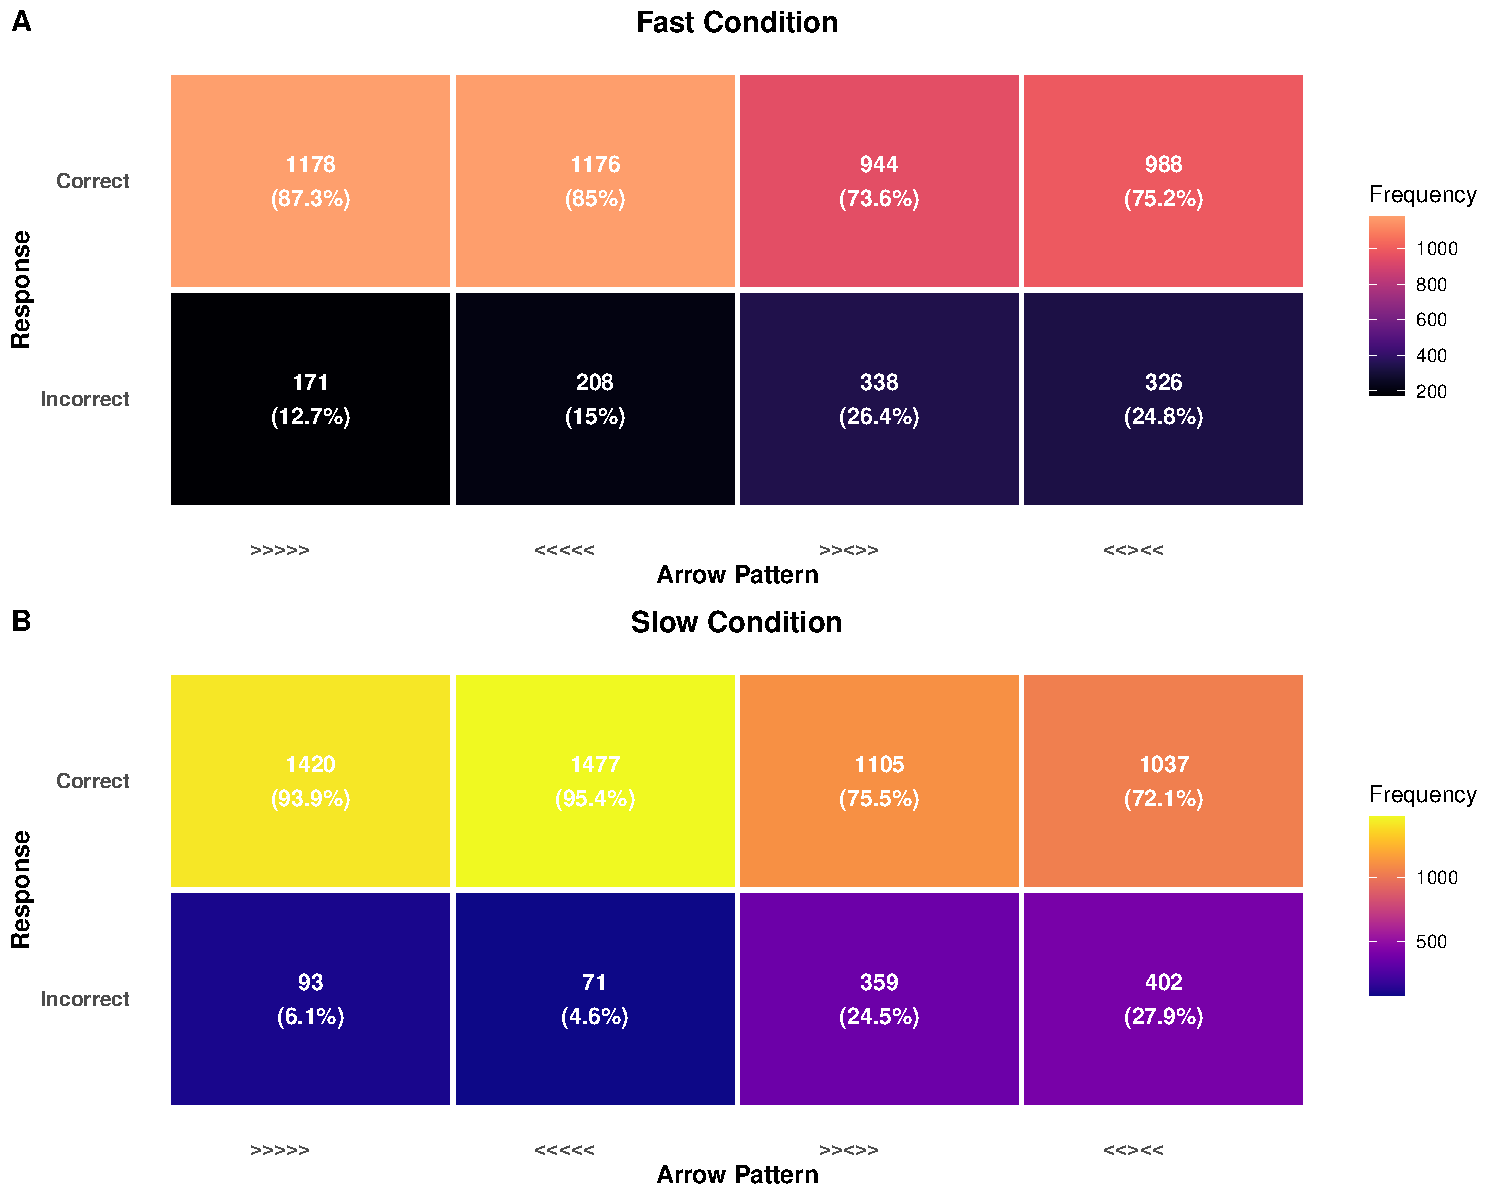
\includegraphics[keepaspectratio]{TrabajoFinal_files/figure-pdf/flanker-accuracy-heatmaps-1.pdf}}

}

\caption{Distribution of correct and incorrect responses in the Flanker
task. (A) Fast condition and (B) Slow condition show the frequency and
percentage of responses for each arrow pattern (congruent:
\textgreater\textgreater\textgreater\textgreater\textgreater{} and
\textless\textless\textless\textless\textless; incongruent:
\textgreater\textgreater\textless\textgreater\textgreater{} and
\textless\textless\textgreater\textless\textless).}

\end{figure}%

\begin{figure}[H]

{\centering \pandocbounded{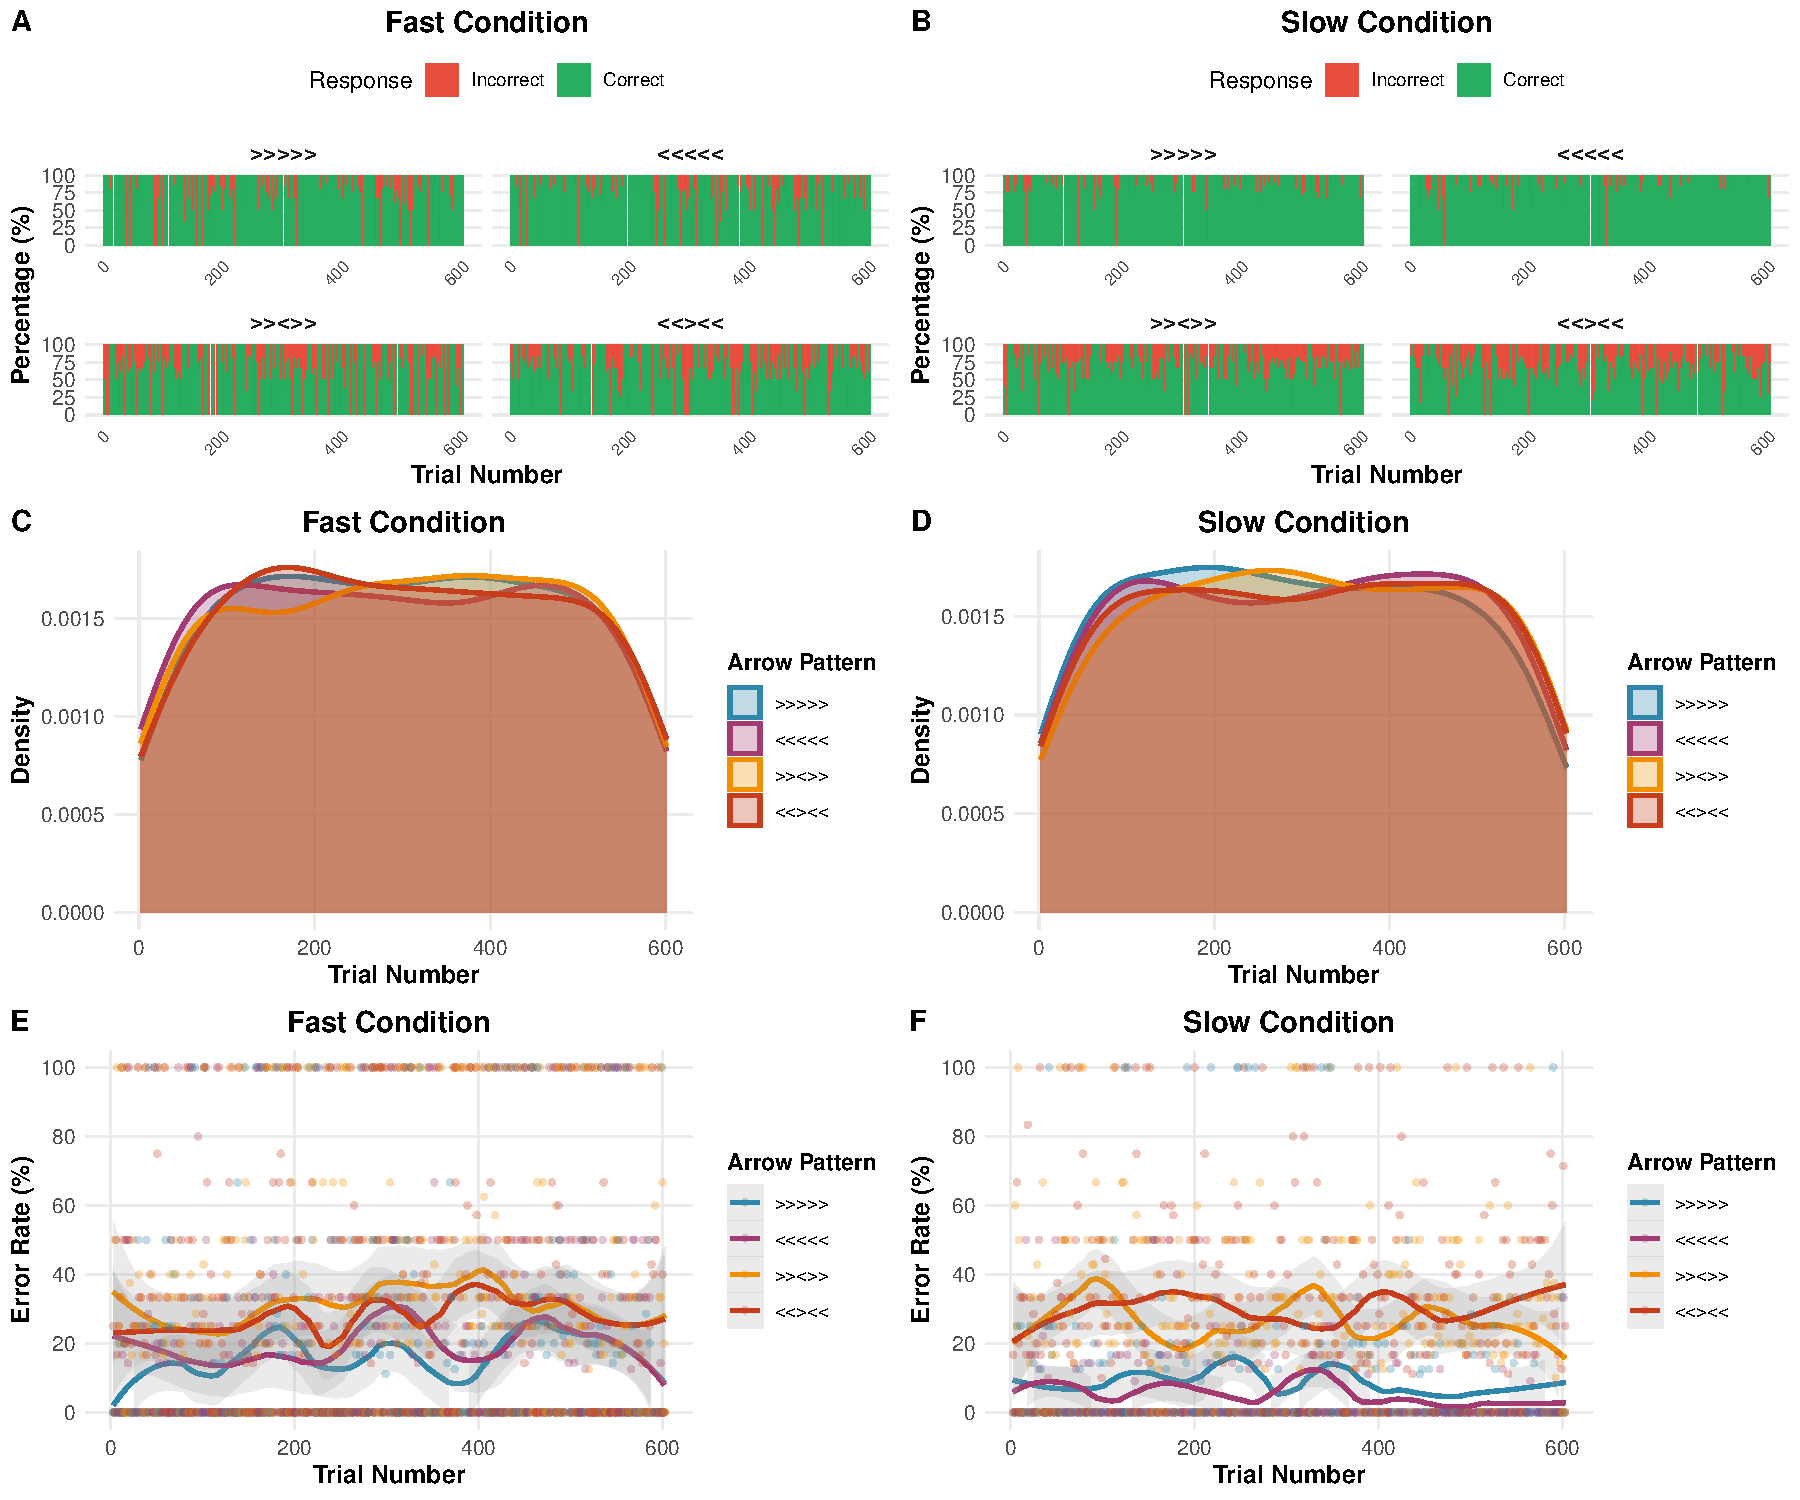
\includegraphics[keepaspectratio]{TrabajoFinal_files/figure-pdf/flanker-trial-progression-1.pdf}}

}

\caption{Trial-by-trial analysis of the Flanker task. (A-B) Response
distribution across trials for each arrow pattern in fast and slow
conditions. (C-D) Distribution of arrow patterns across experimental
trials. (E-F) Smoothed error rates showing learning curves for each
arrow pattern.}

\end{figure}%

\begin{figure}[H]

{\centering \pandocbounded{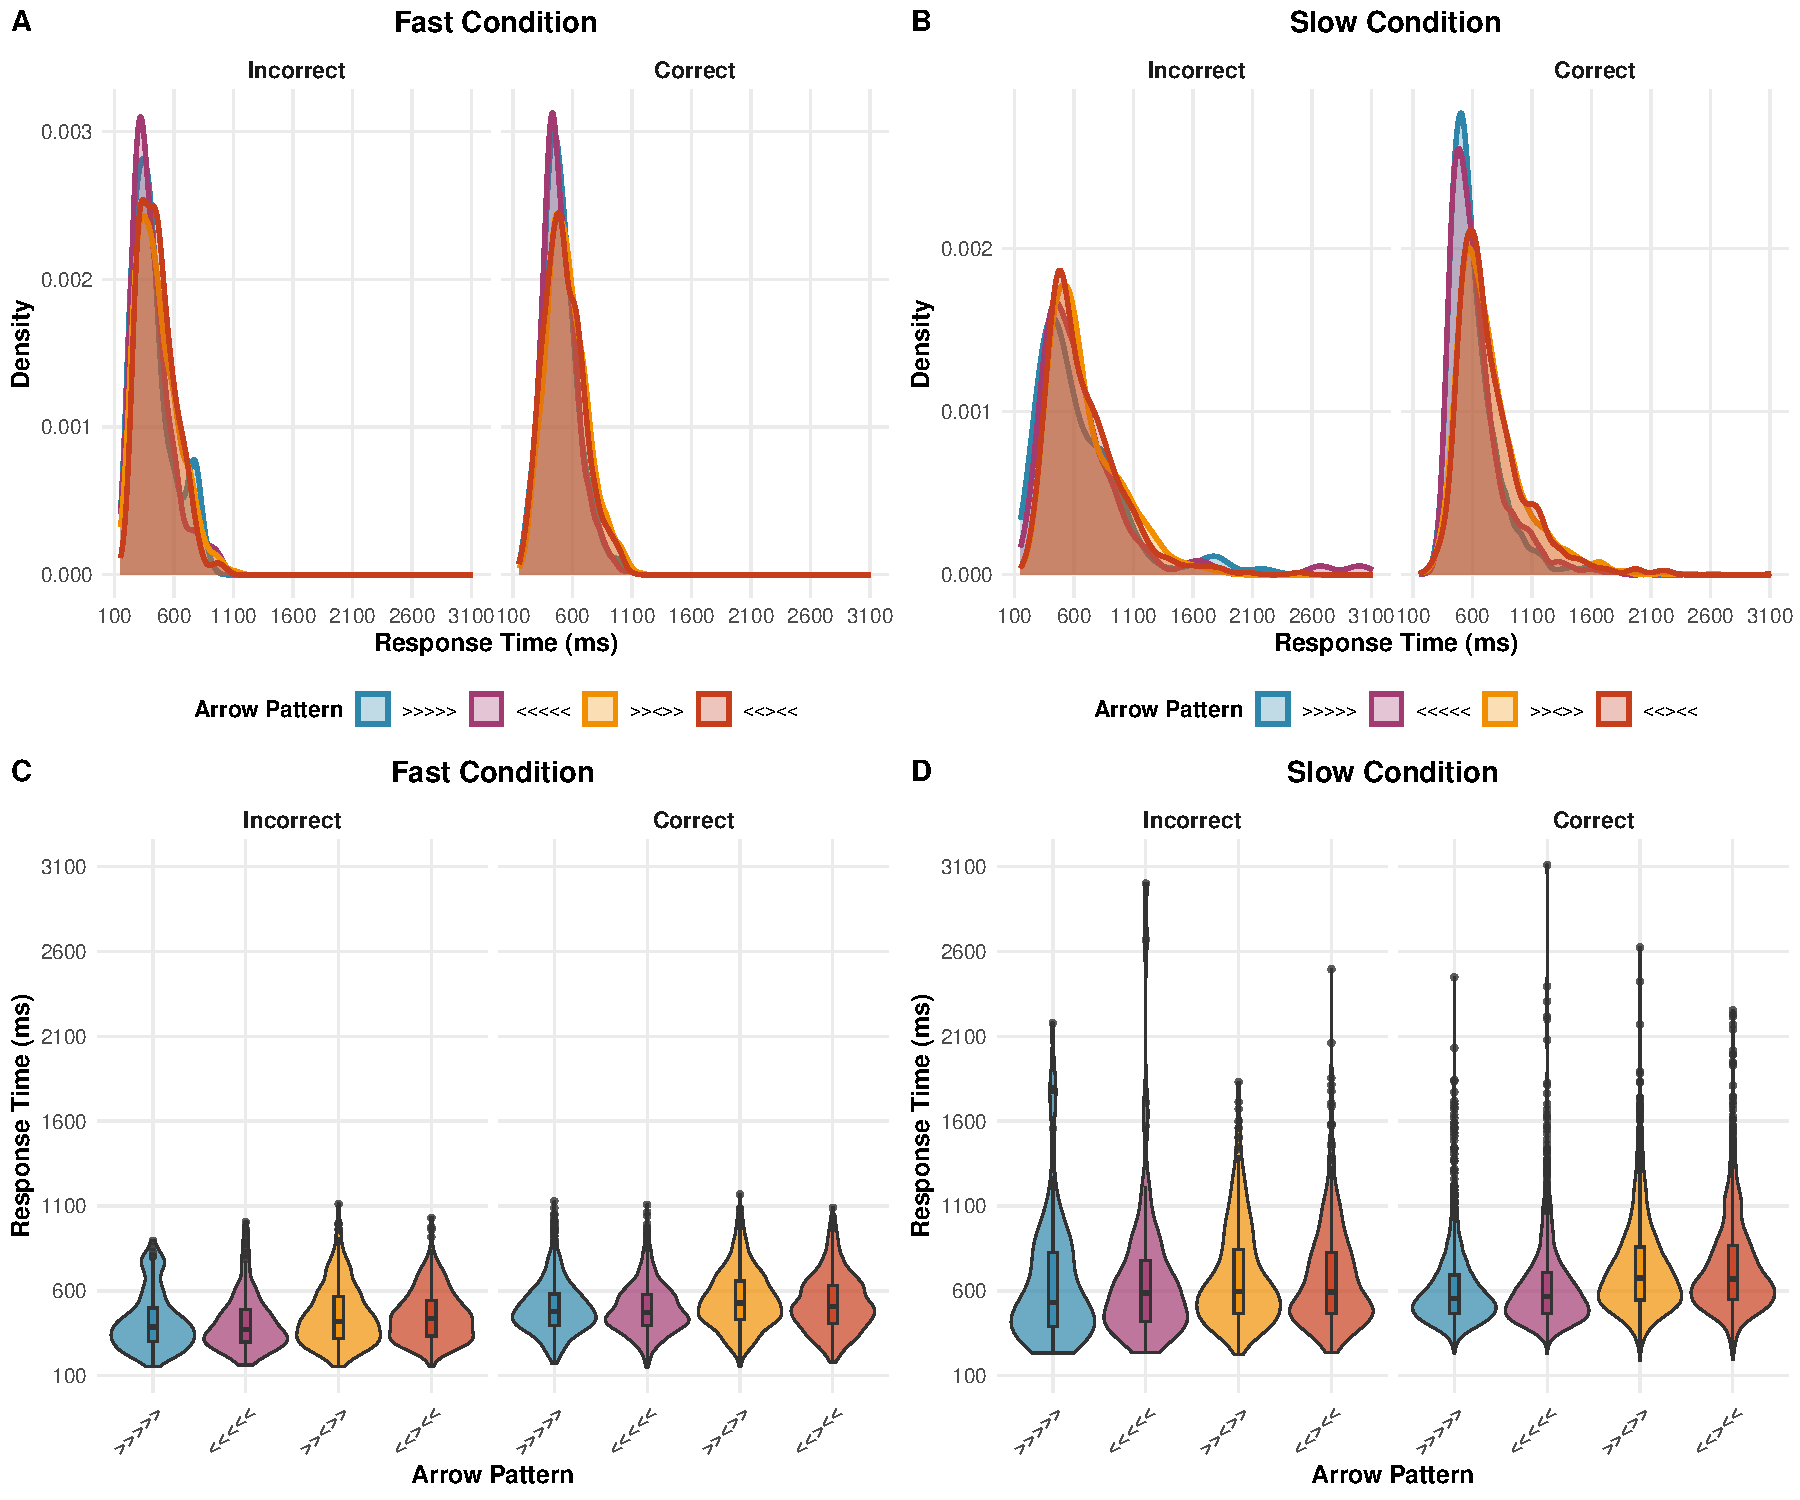
\includegraphics[keepaspectratio]{TrabajoFinal_files/figure-pdf/flanker-rt-distributions-1.pdf}}

}

\caption{Response time distributions in the Flanker task. (A-B) Density
plots showing RT distributions for each arrow pattern, separated by
response accuracy. (C-D) Violin plots with embedded boxplots showing RT
distributions and outliers for each condition.}

\end{figure}%

\begin{figure}[H]

{\centering \pandocbounded{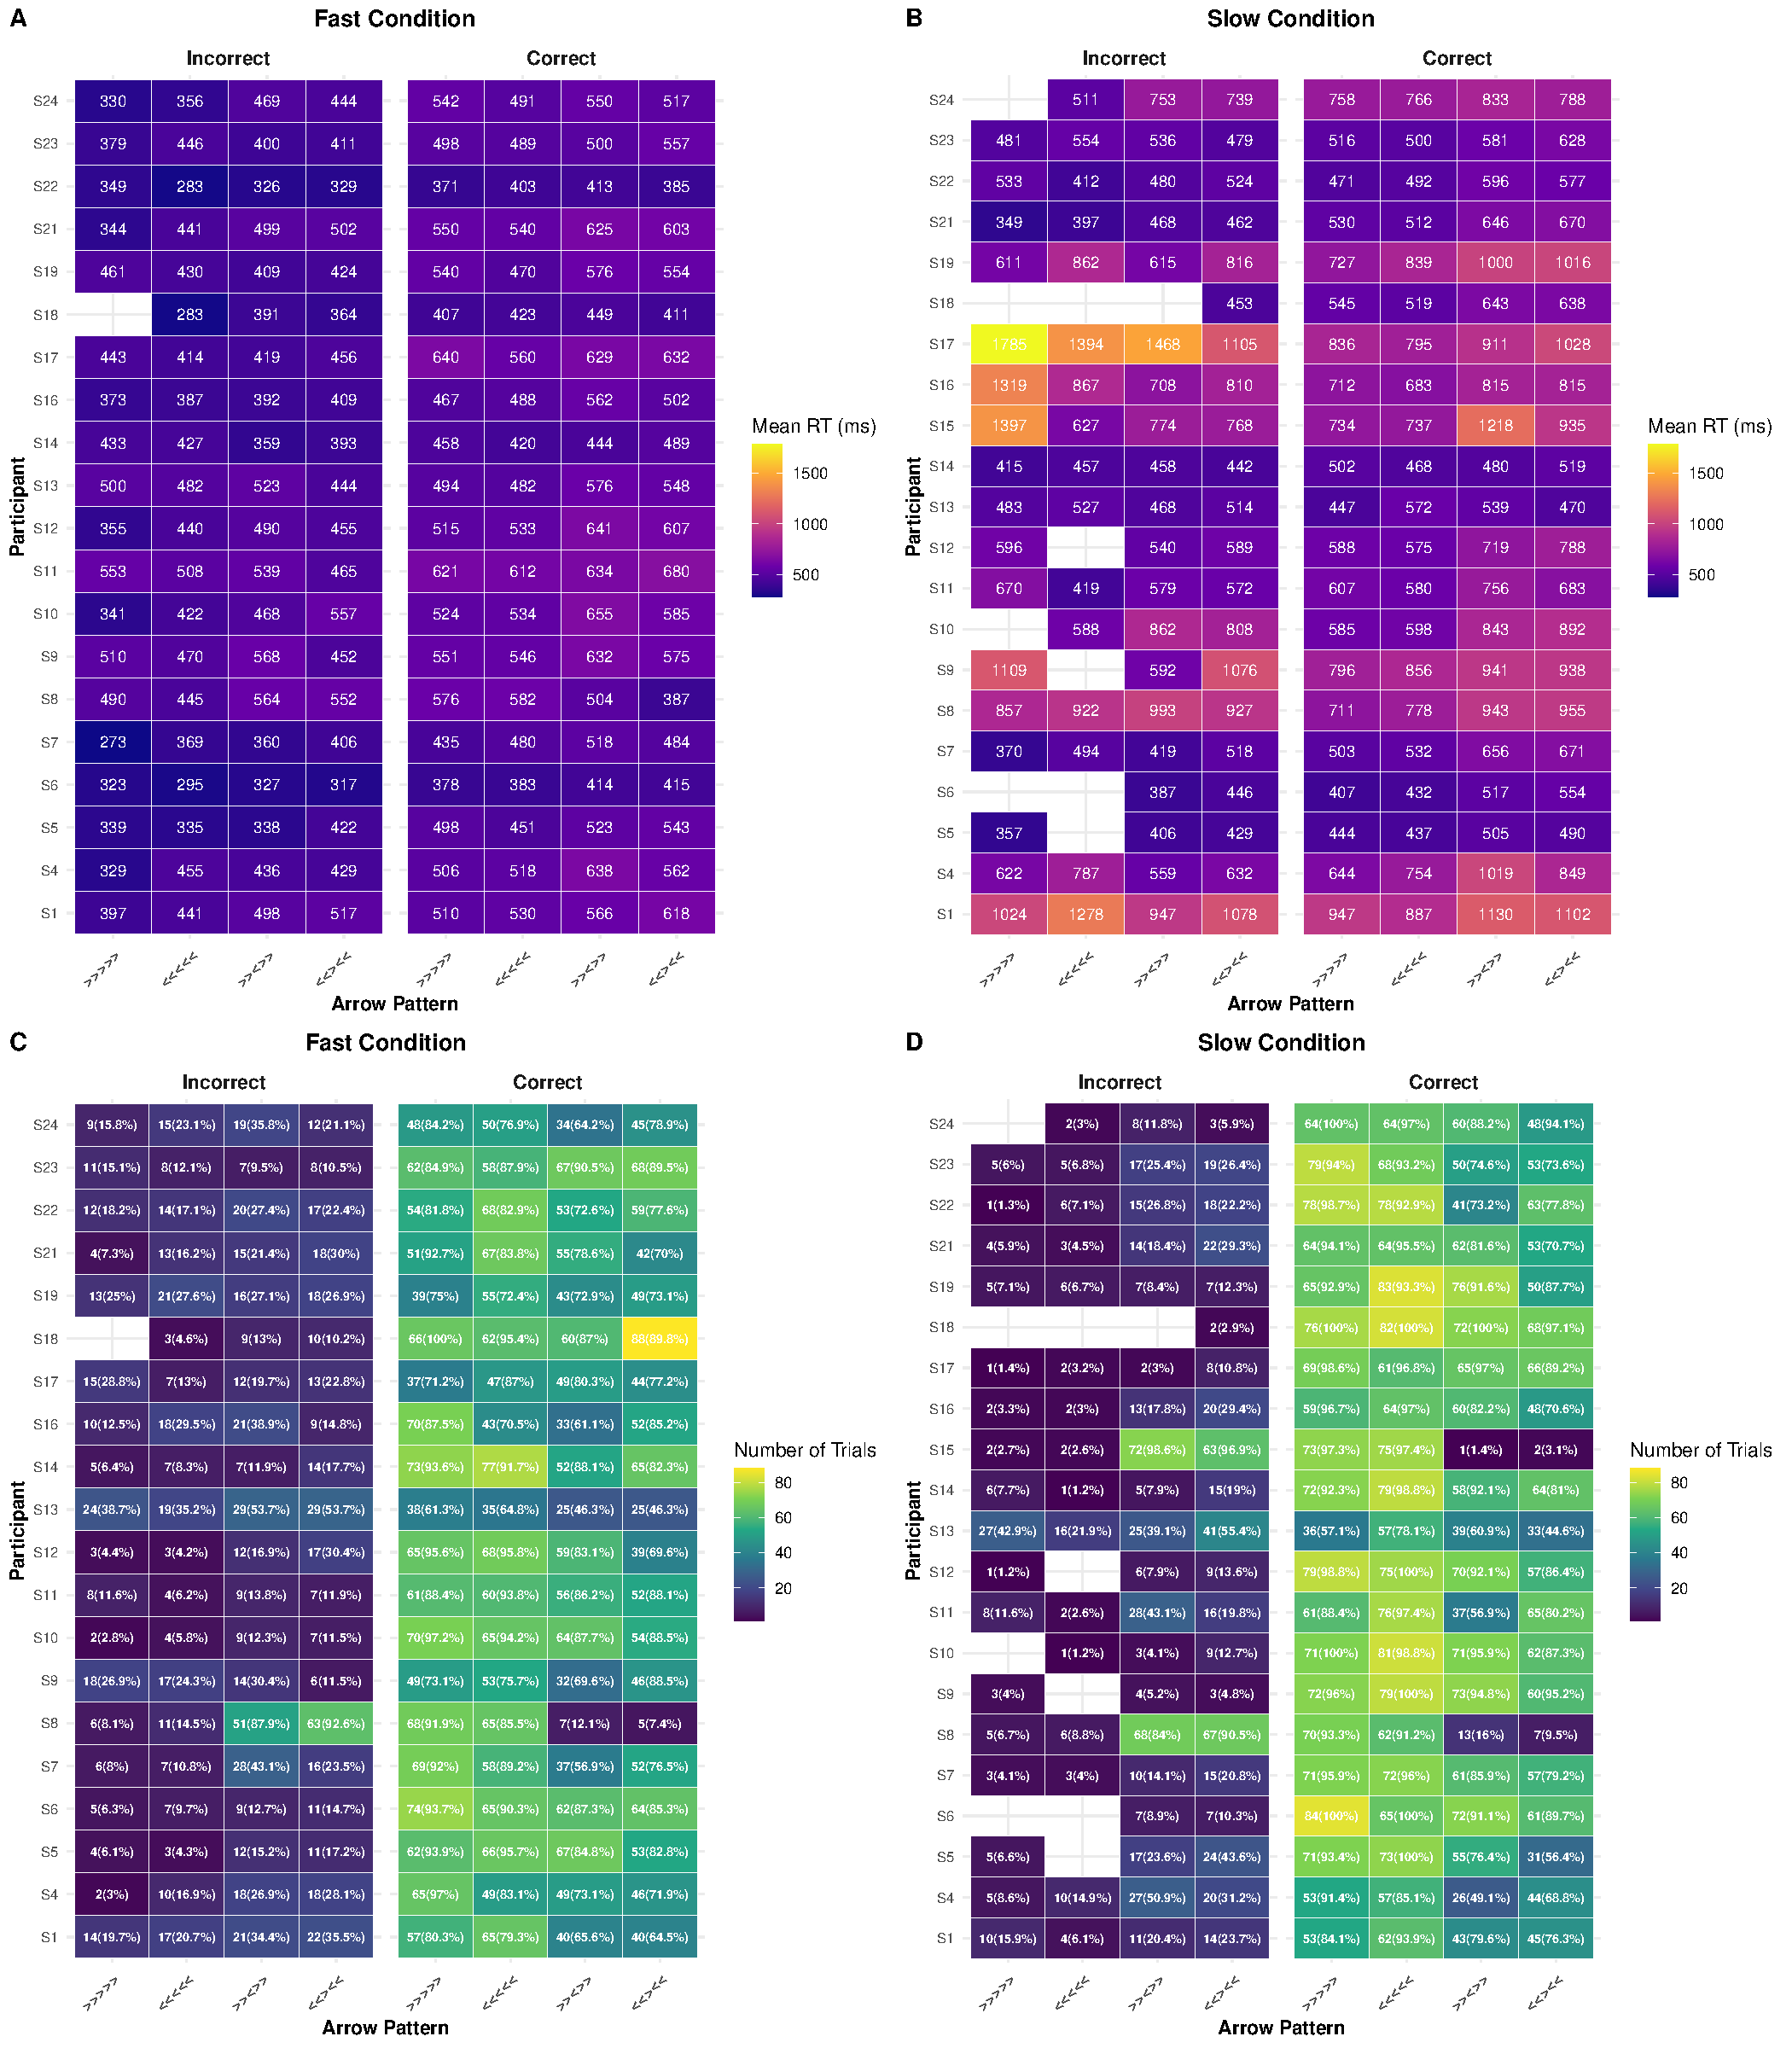
\includegraphics[keepaspectratio]{TrabajoFinal_files/figure-pdf/flanker-individual-analysis-1.pdf}}

}

\caption{Individual participant analysis for the Flanker task. (A-B)
Mean response times and (C-D) trial counts for each participant across
arrow patterns and response types. Heatmaps show individual differences
in performance patterns.}

\end{figure}%

\begin{figure}[H]

{\centering \pandocbounded{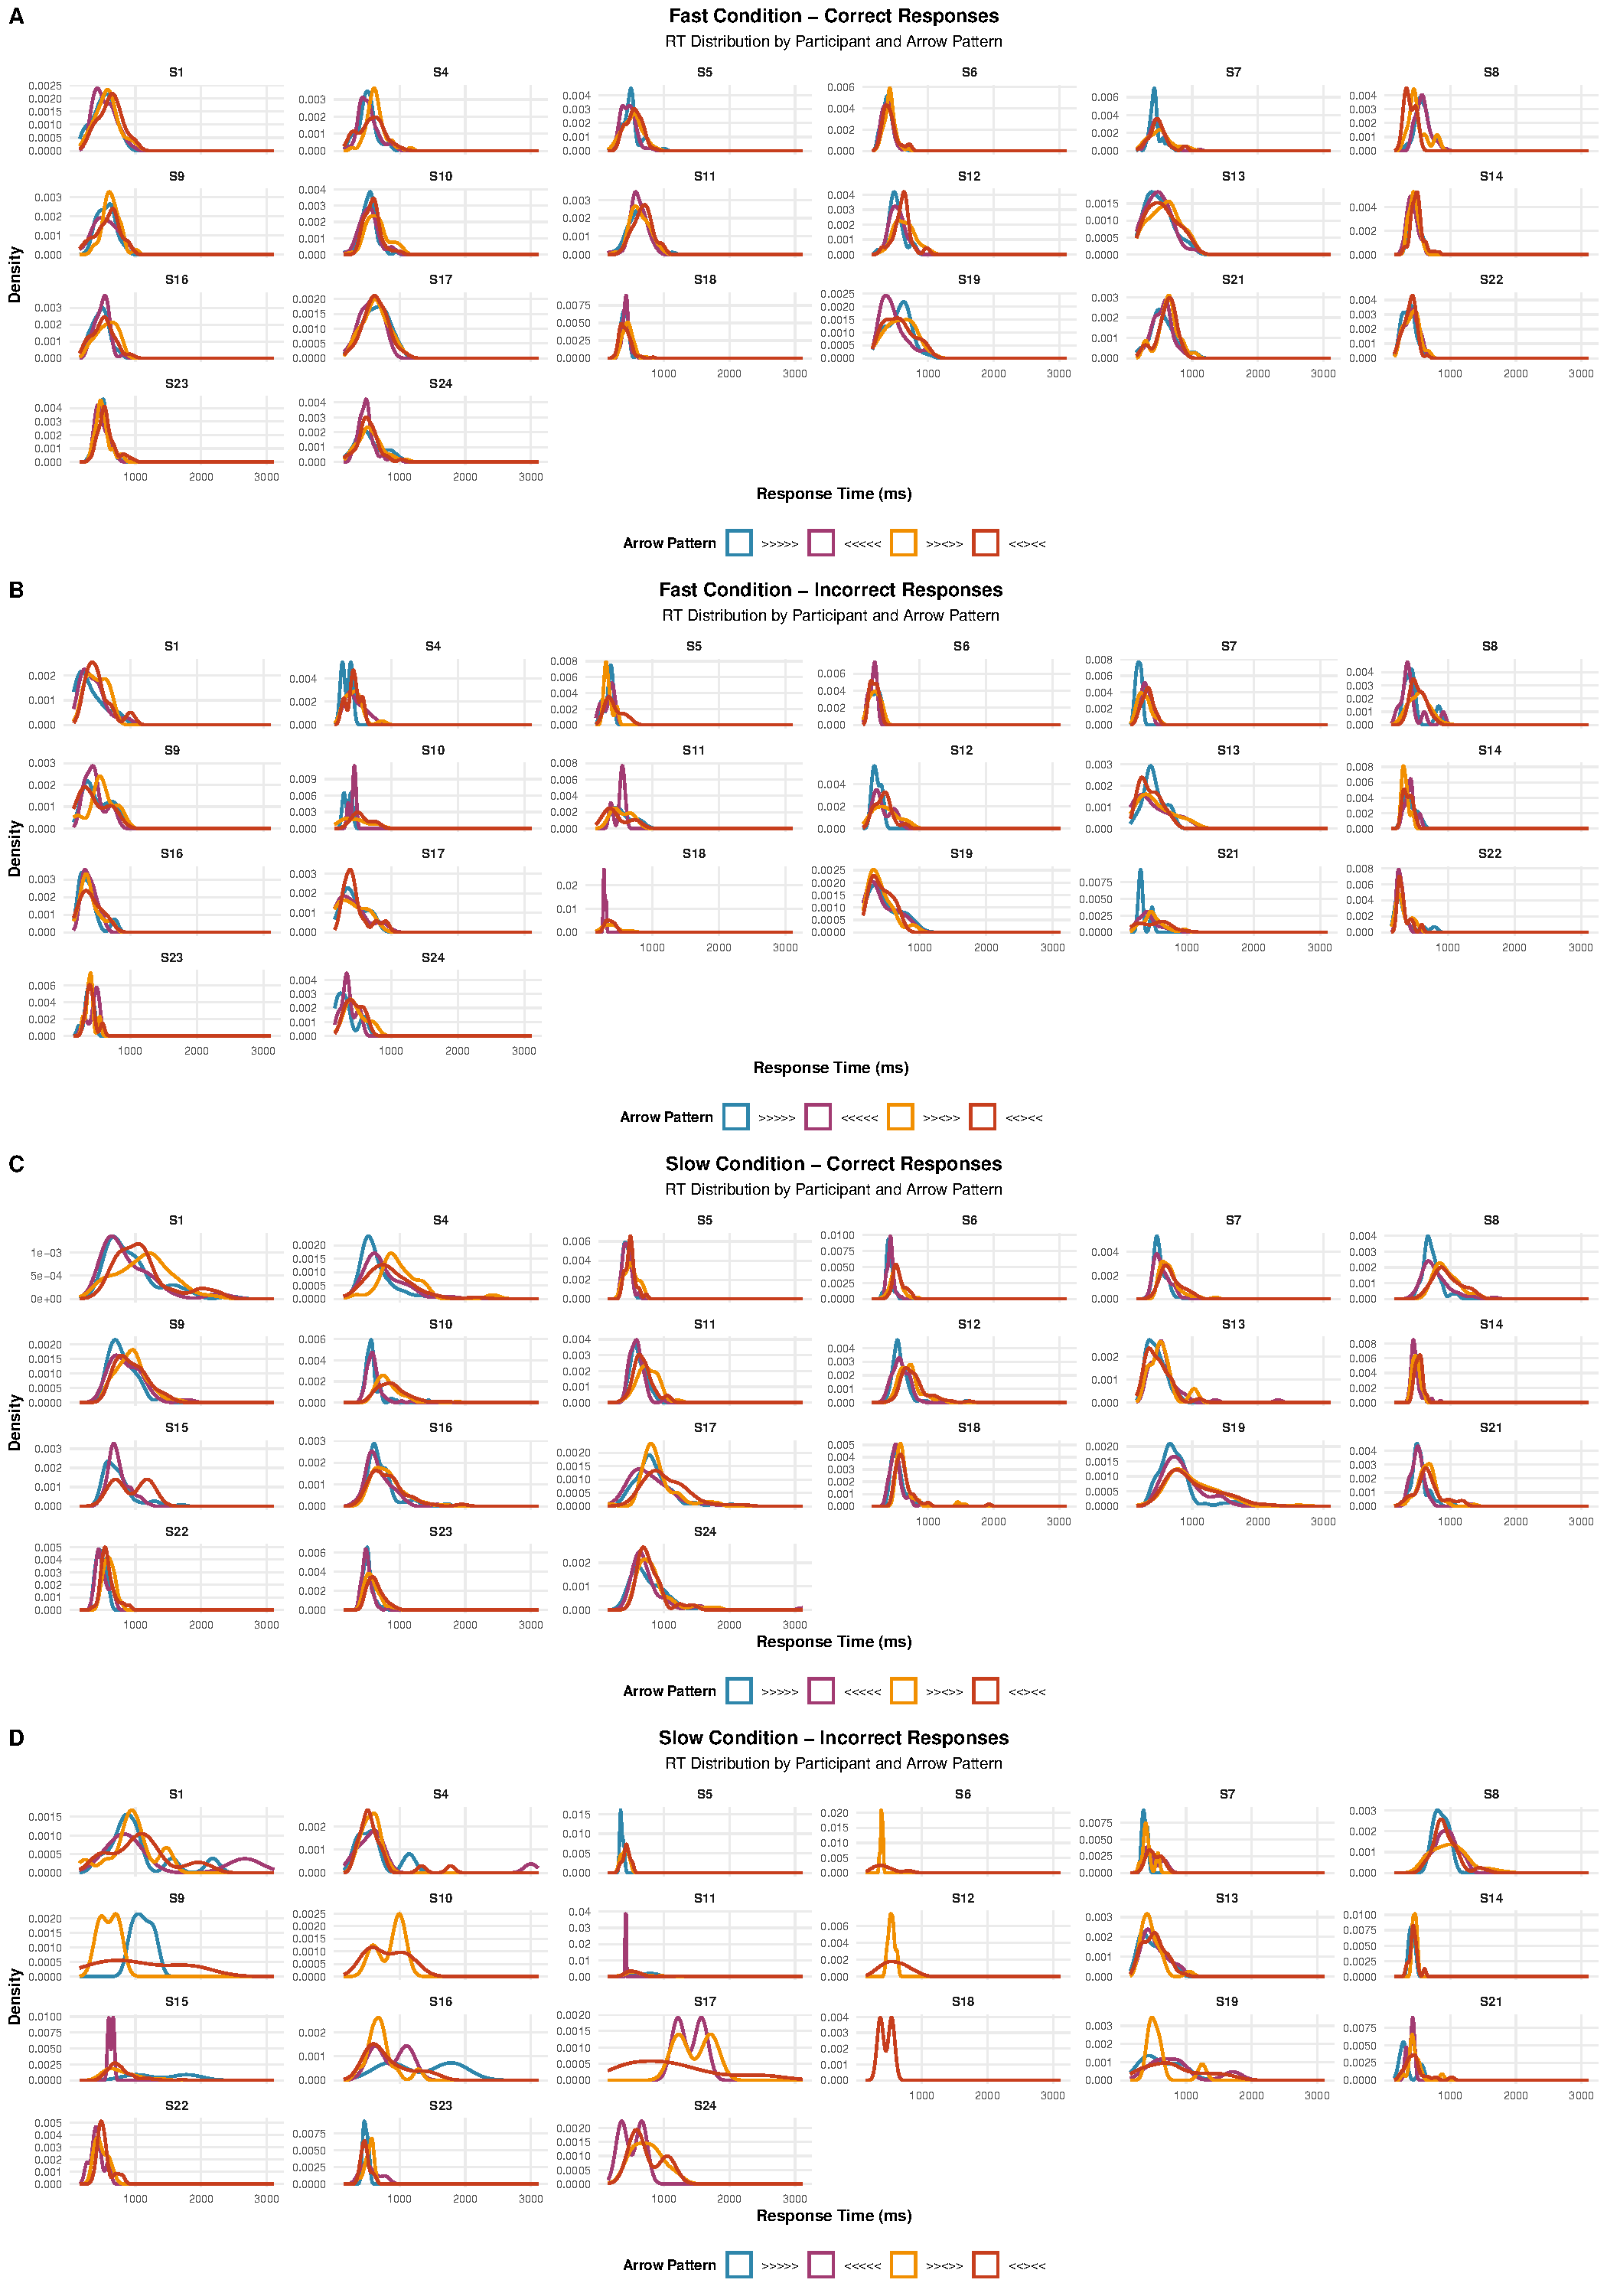
\includegraphics[keepaspectratio]{TrabajoFinal_files/figure-pdf/flanker-individual-rt-density-1.pdf}}

}

\caption{Individual participant RT density distributions for the Flanker
task. Panels show RT distributions for each participant separated by
arrow pattern and response accuracy in (A-B) Fast and (C-D) Slow
conditions.}

\end{figure}%

\subsection{La Tarea Go/No-Go: Un Paradigma para la Inhibición de la
Respuesta}\label{la-tarea-gono-go-un-paradigma-para-la-inhibiciuxf3n-de-la-respuesta}

La tarea Go/No-Go representa un paradigma experimental clásico para el
estudio de la inhibición de respuesta, un componente fundamental del
control ejecutivo \cite{Donders1969}. En contraste con la tarea Flanker
que evalúa la resolución de conflictos entre respuestas competidoras, la
tarea Go/No-Go examina la capacidad de suprimir completamente una
respuesta motora cuando las demandas contextuales así lo requieren
\cite{Verbruggen2019}. La estructura de esta tarea genera una tendencia
de respuesta dominante mediante la presentación frecuente de estímulos
``Go'' que requieren una respuesta rápida, intercalados con estímulos
``No-Go'' infrecuentes que demandan la inhibición de esta respuesta
automatizada.

En la implementación actual del experimento, se empleó una proporción
típica de 80\% ensayos Go y 20\% ensayos No-Go, diseñada para establecer
una fuerte impulsividad de respuesta que hace que la inhibición en los
ensayos No-Go sea cognitivamente demandante \cite{Wessel2018}. Esta
proporción asimétrica es crítica para el paradigma, ya que una
distribución más equilibrada reduciría la velocidada de la respuesta y,
consecuentemente, la demanda de control inhibitorio. Al igual que en la
tarea Flanker, se implementó una manipulación factorial de la velocidad
de respuesta, con condiciones rápida y lenta, permitiendo examinar cómo
la presión temporal afecta los procesos inhibitorios.

La Figura 6 presenta la distribución fundamental de respuestas correctas
e incorrectas para los estímulos Go y No-Go en ambas condiciones de
velocidad. En la condición rápida (Figura 6A), los datos revelan un
patrón de rendimiento característico del paradigma. Los ensayos Go
muestran una precisión extremadamente alta del 97.5\% (5,623 respuestas
correctas de 5,768 ensayos), confirmando el establecimiento exitoso de
la respuesta. Esta alta tasa de aciertos en los ensayos Go contrasta
marcadamente con el rendimiento en los ensayos No-Go, donde se observa
una tasa de falsas alarmas del 17.9\% (252 errores de 1,406 ensayos),
equivalente a una precisión del 82.1\% en la inhibición de respuesta.

La condición lenta (Figura 6B) presenta un patrón inesperado que merece
análisis detallado. Mientras que la precisión en los ensayos Go
disminuye ligeramente al 93.5\% (5,216 correctas de 5,578 ensayos), la
tasa de falsas alarmas en los ensayos No-Go aumenta considerablemente al
29.9\% (409 errores de 1,369 ensayos). Este incremento en las falsas
alarmas bajo condiciones de menor presión temporal parece
contraintuitivo, ya que cabría esperar que el tiempo adicional
facilitara la inhibición exitosa. Sin embargo, este fenómeno ha sido
documentado en la literatura y puede atribuirse a varios factores
interrelacionados \cite{Littman2017}.

El análisis temporal presentado en la Figura 7 proporciona información
valiosa sobre la dinámica del control inhibitorio a lo largo del
experimento. Los paneles superiores (Figuras 7A-B) muestran la
distribución de respuestas para cada tipo de estímulo a través de los
aproximadamente 300 ensayos por condición. Un aspecto notable es la
distribución temporal de los errores. En los ensayos Go, los escasos
errores (omisiones) aparecen distribuidos de manera relativamente
uniforme a lo largo del experimento, sugiriendo lapsos atencionales
ocasionales más que un patrón sistemático de fatiga o aprendizaje. Por
el contrario, las falsas alarmas en los ensayos No-Go muestran una
distribución más variable, con períodos de inhibición exitosa alternando
con rachas de errores, particularmente en la condición lenta.

Las curvas de error suavizadas (Figuras 7E-F) revelan tendencias
temporales diferenciadas entre las condiciones. En la condición rápida,
la tasa de error para los ensayos Go se mantiene establemente baja
alrededor del 2-3\% durante todo el experimento. La tasa de falsas
alarmas para los ensayos No-Go muestra mayor variabilidad, oscilando
entre 15-25\%, pero sin una tendencia clara de mejora o deterioro con la
práctica. Este patrón sugiere que el control inhibitorio bajo presión
temporal representa una demanda cognitiva constante que no se beneficia
significativamente de la experiencia dentro de la sesión experimental.

La condición lenta presenta un perfil temporal más complejo. Las tasas
de error en los ensayos Go muestran mayor variabilidad, fluctuando entre
5-10\%, posiblemente reflejando fluctuaciones en la atención sostenida
cuando la tarea permite un ritmo más pausado. Las tasas de falsas
alarmas en los ensayos No-Go son notablemente más altas y variables,
oscilando entre 25-35\% con picos ocasionales que alcanzan el 40\%. Esta
mayor variabilidad temporal en la condición lenta sugiere que la
reducción en la presión temporal puede paradójicamente desestabilizar el
control inhibitorio, posiblemente al permitir mayor variabilidad en las
estrategias de preparación y en los estados atencionales.

El análisis de los tiempos de respuesta, presentado en la Figura 8,
revela aspectos importantes sobre la dinámica temporal de los procesos
de decisión y ejecución. Las distribuciones de densidad (Figuras 8A-B)
muestran perfiles claramente diferenciados entre los aciertos Go y las
falsas alarmas No-Go. Los aciertos Go exhiben distribuciones
relativamente simétricas y compactas, con tendencias centrales alrededor
de 400-450 ms en la condición rápida y 450-500 ms en la condición lenta

Las falsas alarmas No-Go presentan un perfil temporal distintivo. En
ambas condiciones de velocidad, los TRs de las falsas alarmas son
comparables o incluso ligeramente más rápidos que los aciertos Go, con
distribuciones que muestran menor variabilidad. Este patrón es
consistente con la interpretación de que las falsas alarmas resultan de
fallas en el proceso de inhibición, donde la respuesta se ejecuta sin el
control top-down necesario para detenerla. La similitud en los TRs entre
aciertos Go y falsas alarmas No-Go sugiere que ambos reflejan la
ejecución de la misma respuesta motora, diferenciándose únicamente en si
el proceso inhibitorio fue iniciado exitosamente o no.

Los diagramas de violín (Figuras 8C-D) enfatizan estas diferencias
distribucionales y revelan la presencia de valores atípicos
particularmente en la condición lenta. Estos outliers, con TRs
superiores a 1000 ms, son más frecuentes en los aciertos Go de la
condición lenta, sugiriendo lapsos atencionales ocasionales cuando la
presión temporal es reducida. La ausencia relativa de tales outliers en
las falsas alarmas No-Go refuerza la interpretación de que estos errores
resultan de procesos balísticos relativamente automáticos más que de
decisiones deliberadas pero incorrectas.

La Figura 10 presenta un análisis exhaustivo de las diferencias
individuales en el rendimiento de la tarea Go/No-Go. El panel A muestra
el rendimiento en términos de teoría de detección de señales, graficando
la tasa de aciertos (proporción de respuestas correctas en ensayos Go)
contra la tasa de falsas alarmas (proporción de respuestas incorrectas
en ensayos No-Go) para cada participante. La mayoría de los
participantes se agrupan en la esquina superior izquierda del espacio,
indicando altas tasas de aciertos combinadas con tasas de falsas alarmas
relativamente bajas. Sin embargo, existe variabilidad considerable, con
algunos participantes mostrando tasas de falsas alarmas superiores al
40\% mientras mantienen tasas de aciertos cercanas al 100\%.

Los mapas de calor de TR medios (Figura 10B-C) revelan patrones
individuales consistentes en la velocidad de respuesta. Los
participantes que responden rápidamente en los ensayos Go tienden a
mostrar también falsas alarmas rápidas, sugiriendo diferencias estables
en el umbral motor o en la preparación de respuesta. Algunos
participantes como S5 y S11 muestran TRs medios notablemente rápidos
(300-350 ms) en ambos tipos de respuesta, mientras que otros como S18 y
S22 exhiben TRs más conservadores (500-600 ms). Esta consistencia
intra-individual en la velocidad de respuesta, independientemente del
tipo de ensayo, sugiere que las diferencias individuales en la tarea
Go/No-Go pueden estar más relacionadas con parámetros motores generales
que con la eficiencia específica del control inhibitorio.

El análisis de precisión por participante (Figura 10D-E) revela
heterogeneidad sustancial en la capacidad inhibitoria. Mientras algunos
participantes como S4 y S17 mantienen tasas de falsas alarmas inferiores
al 10\% en ambas condiciones, otros como S8 y S15 muestran tasas de
falsas alarmas que se aproximan o superan el 50\%, indicando
dificultades significativas con el control inhibitorio. Un hallazgo
particularmente interesante es que la variabilidad entre participantes
es mayor para los ensayos No-Go que para los ensayos Go, sugiriendo que
las diferencias individuales en el control cognitivo se manifiestan más
claramente en situaciones que requieren inhibición activa que en
aquellas que requieren ejecución de respuesta.

La comparación entre condiciones de velocidad a nivel individual revela
patrones no uniformes. Mientras algunos participantes muestran el patrón
grupal de peor inhibición en la condición lenta, otros muestran el
patrón opuesto o ninguna diferencia entre condiciones. Esta
heterogeneidad en los efectos de la manipulación de velocidad sugiere
que los participantes pueden adoptar diferentes estrategias o tener
diferentes vulnerabilidades a los factores que contribuyen al incremento
paradójico de falsas alarmas en la condición lenta.

\begin{figure}[H]

{\centering \pandocbounded{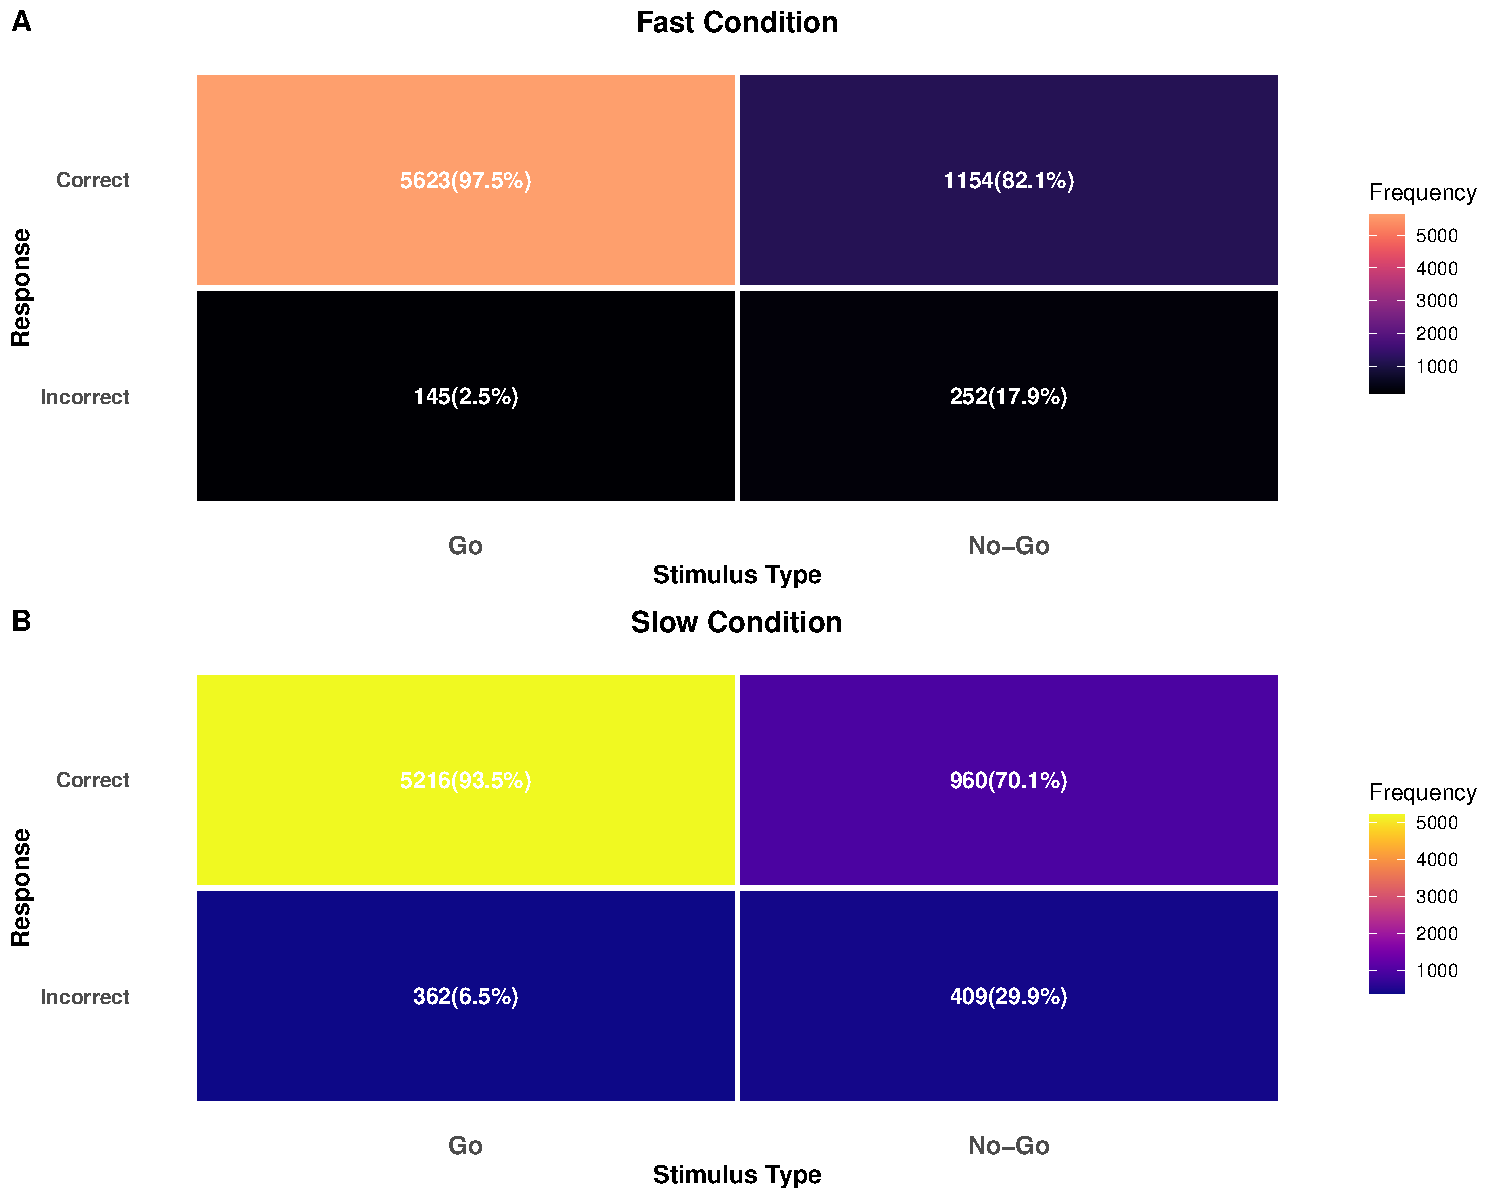
\includegraphics[keepaspectratio]{TrabajoFinal_files/figure-pdf/gonogo-accuracy-analysis-1.pdf}}

}

\caption{Distribution of correct and incorrect responses in the Go/No-Go
task. (A) Fast condition and (B) Slow condition show the frequency and
percentage of responses for Go and No-Go trials.}

\end{figure}%

\begin{figure}[H]

{\centering \pandocbounded{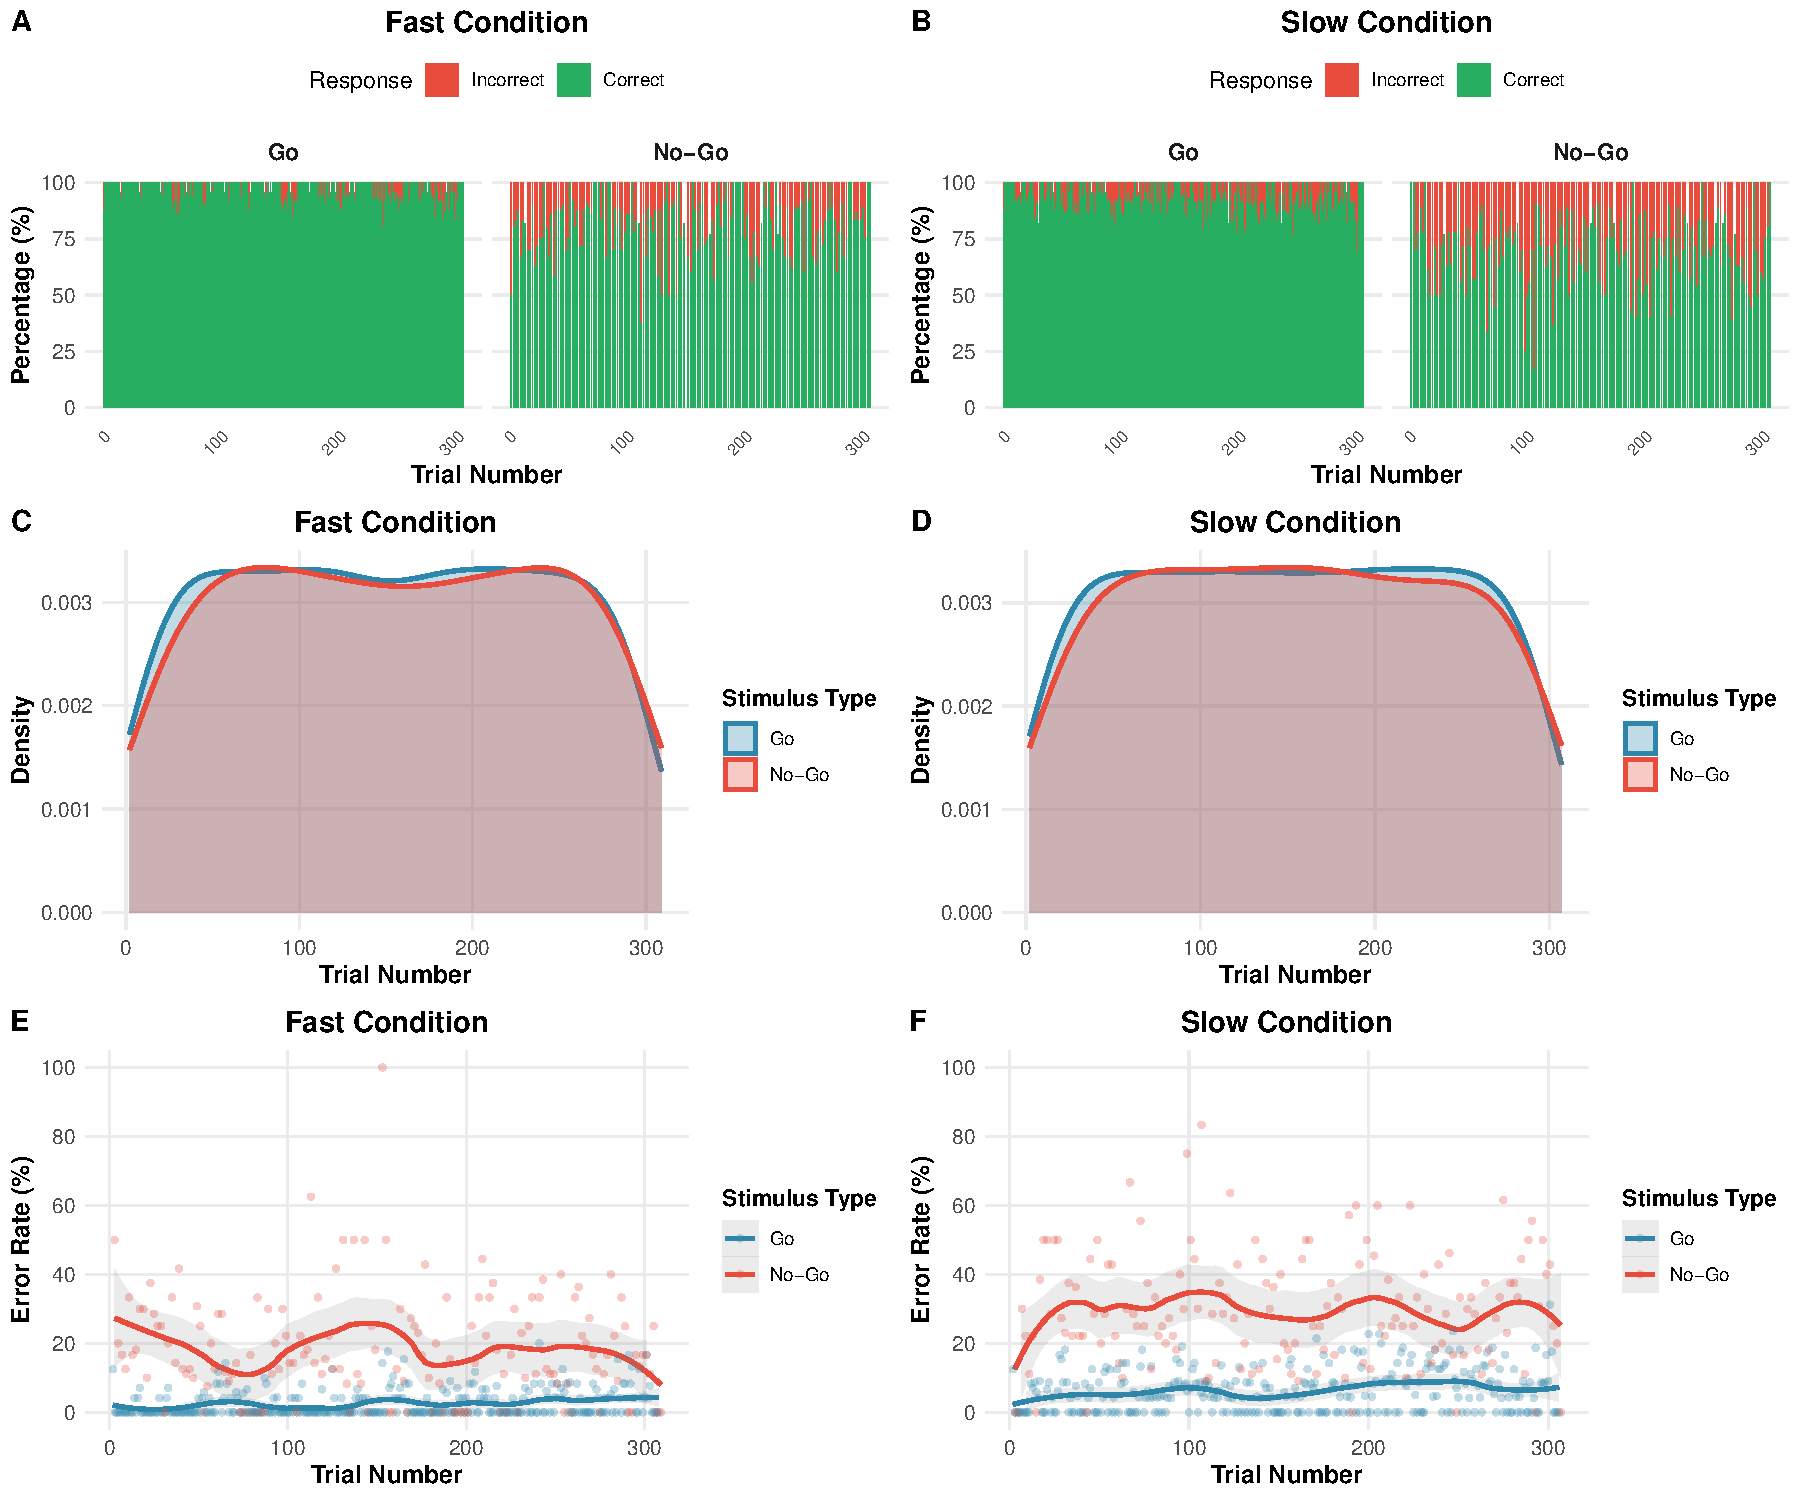
\includegraphics[keepaspectratio]{TrabajoFinal_files/figure-pdf/gonogo-trial-progression-1.pdf}}

}

\caption{Trial-by-trial analysis of the Go/No-Go task. (A-B) Response
distribution across trials for Go and No-Go stimuli. (C-D) Distribution
of stimulus types across trials. (E-F) Error rates showing performance
changes over time.}

\end{figure}%

\begin{figure}[H]

{\centering \pandocbounded{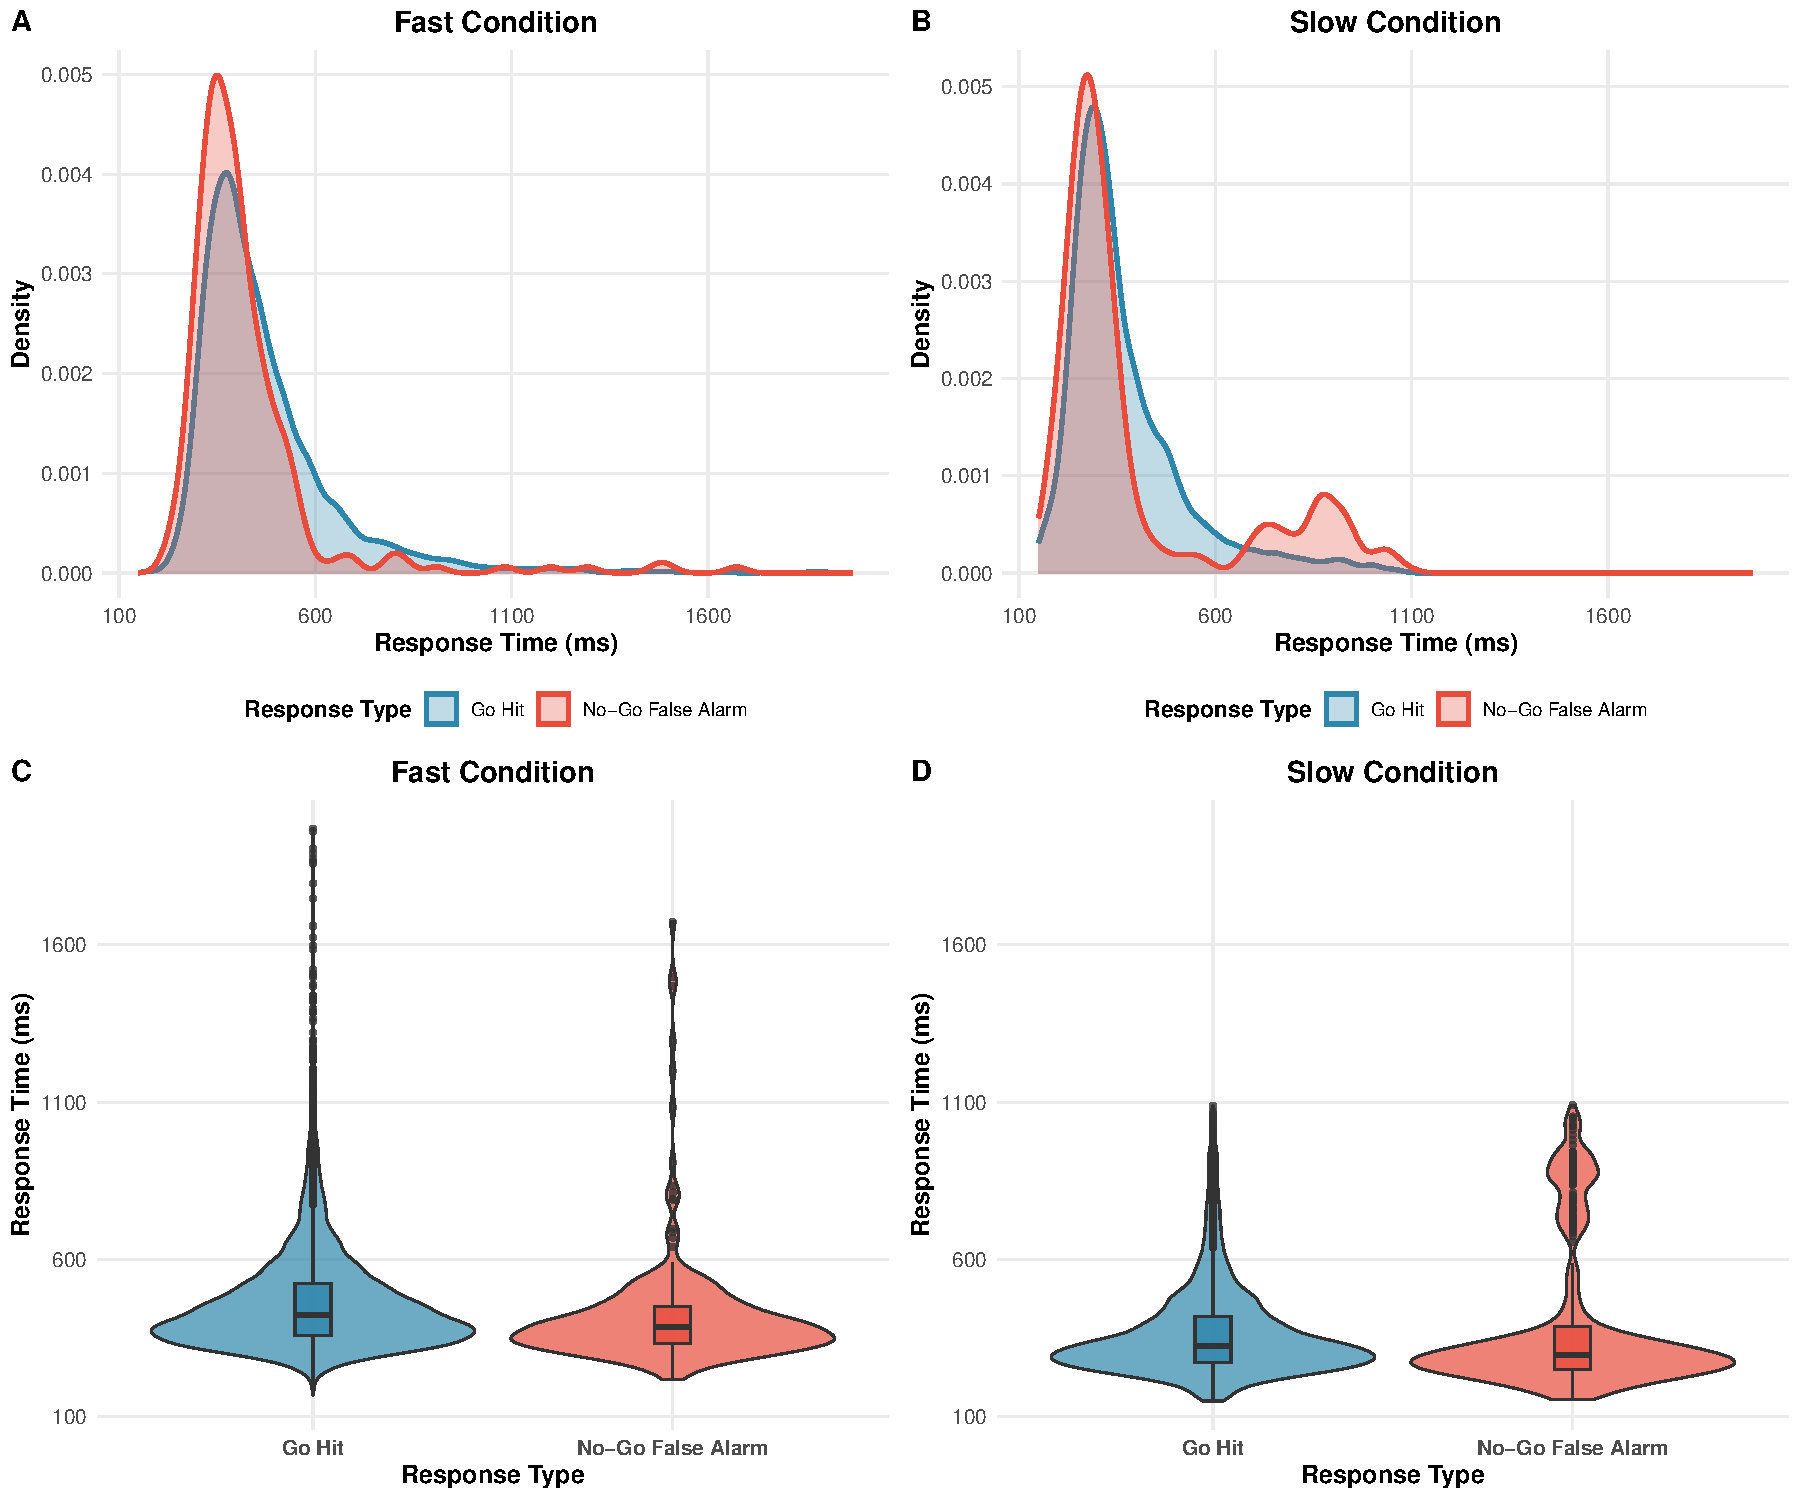
\includegraphics[keepaspectratio]{TrabajoFinal_files/figure-pdf/gonogo-rt-distributions-1.pdf}}

}

\caption{Response time distributions in the Go/No-Go task. (A-B) Density
plots showing RT distributions for Go hits and No-Go false alarms. (C-D)
Violin plots with embedded boxplots showing RT distributions for each
response type.}

\end{figure}%

\begin{figure}[H]

{\centering \pandocbounded{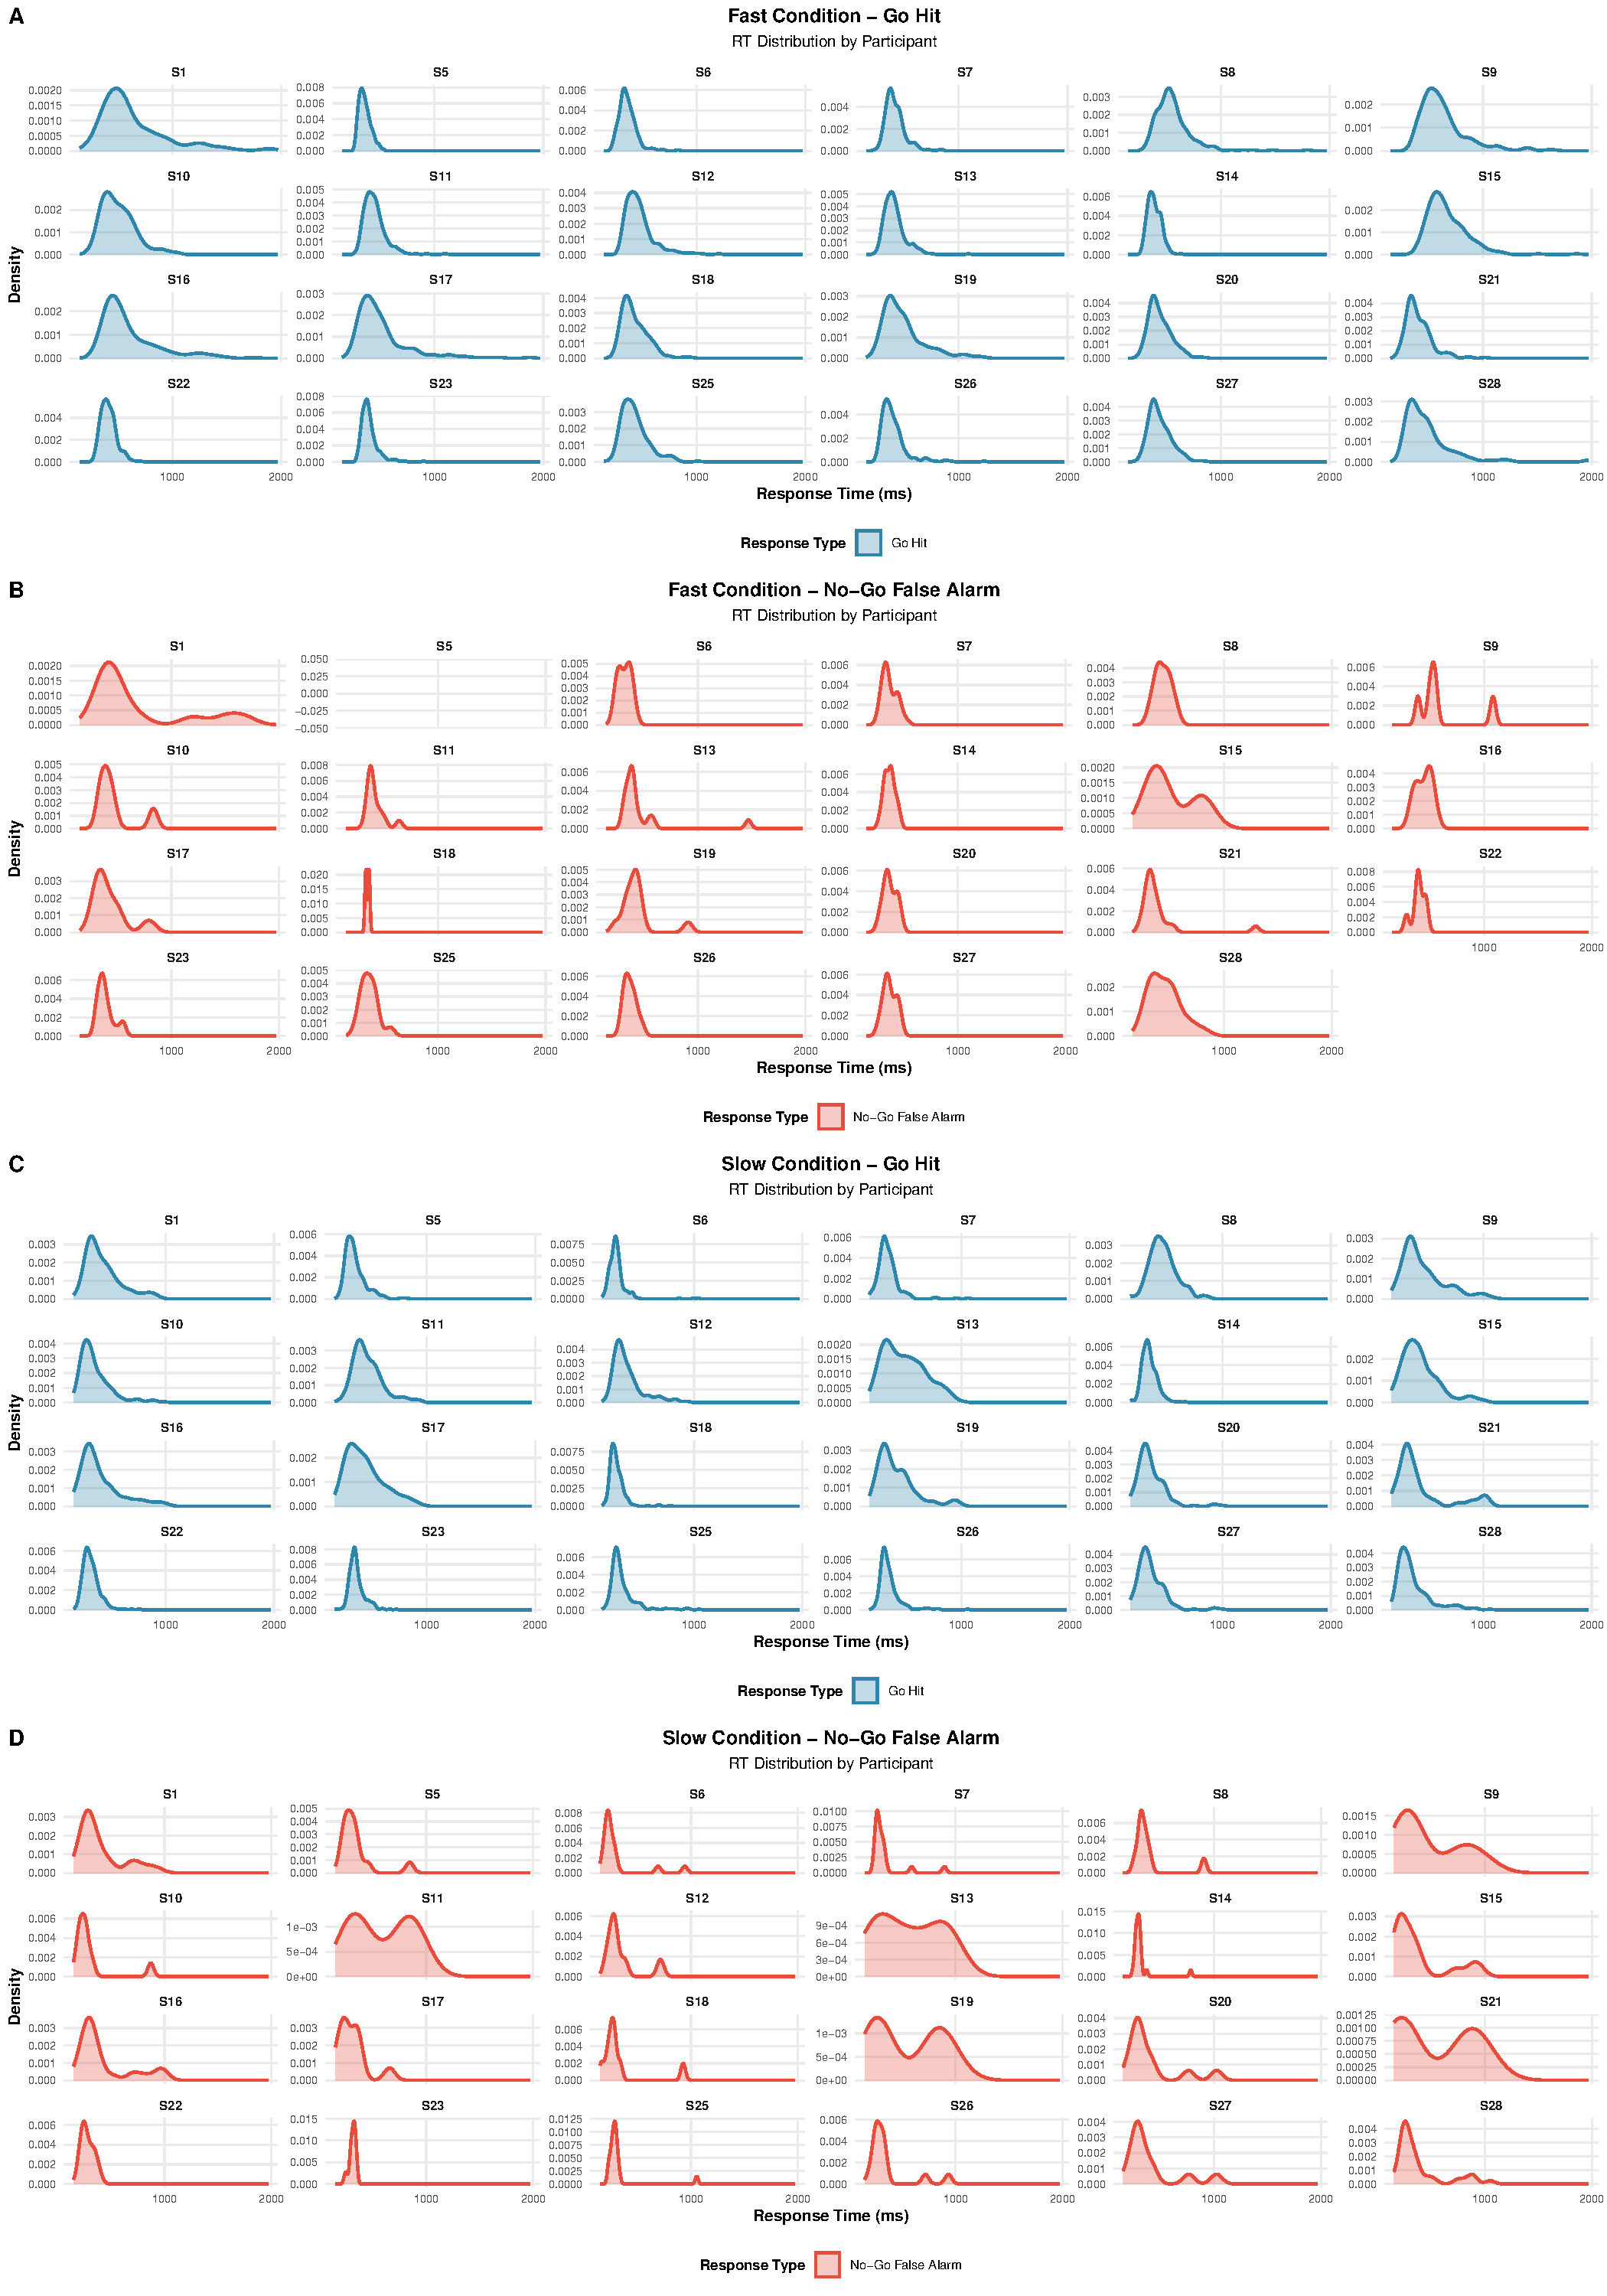
\includegraphics[keepaspectratio]{TrabajoFinal_files/figure-pdf/gonogo-individual-rt-density-1.pdf}}

}

\caption{Individual participant RT density distributions for the
Go/No-Go task. Panels show RT distributions for each participant
separated by response type (Go Hit vs No-Go False Alarm) in (A-B) Fast
and (C-D) Slow conditions.}

\end{figure}%

\begin{figure}[H]

{\centering \pandocbounded{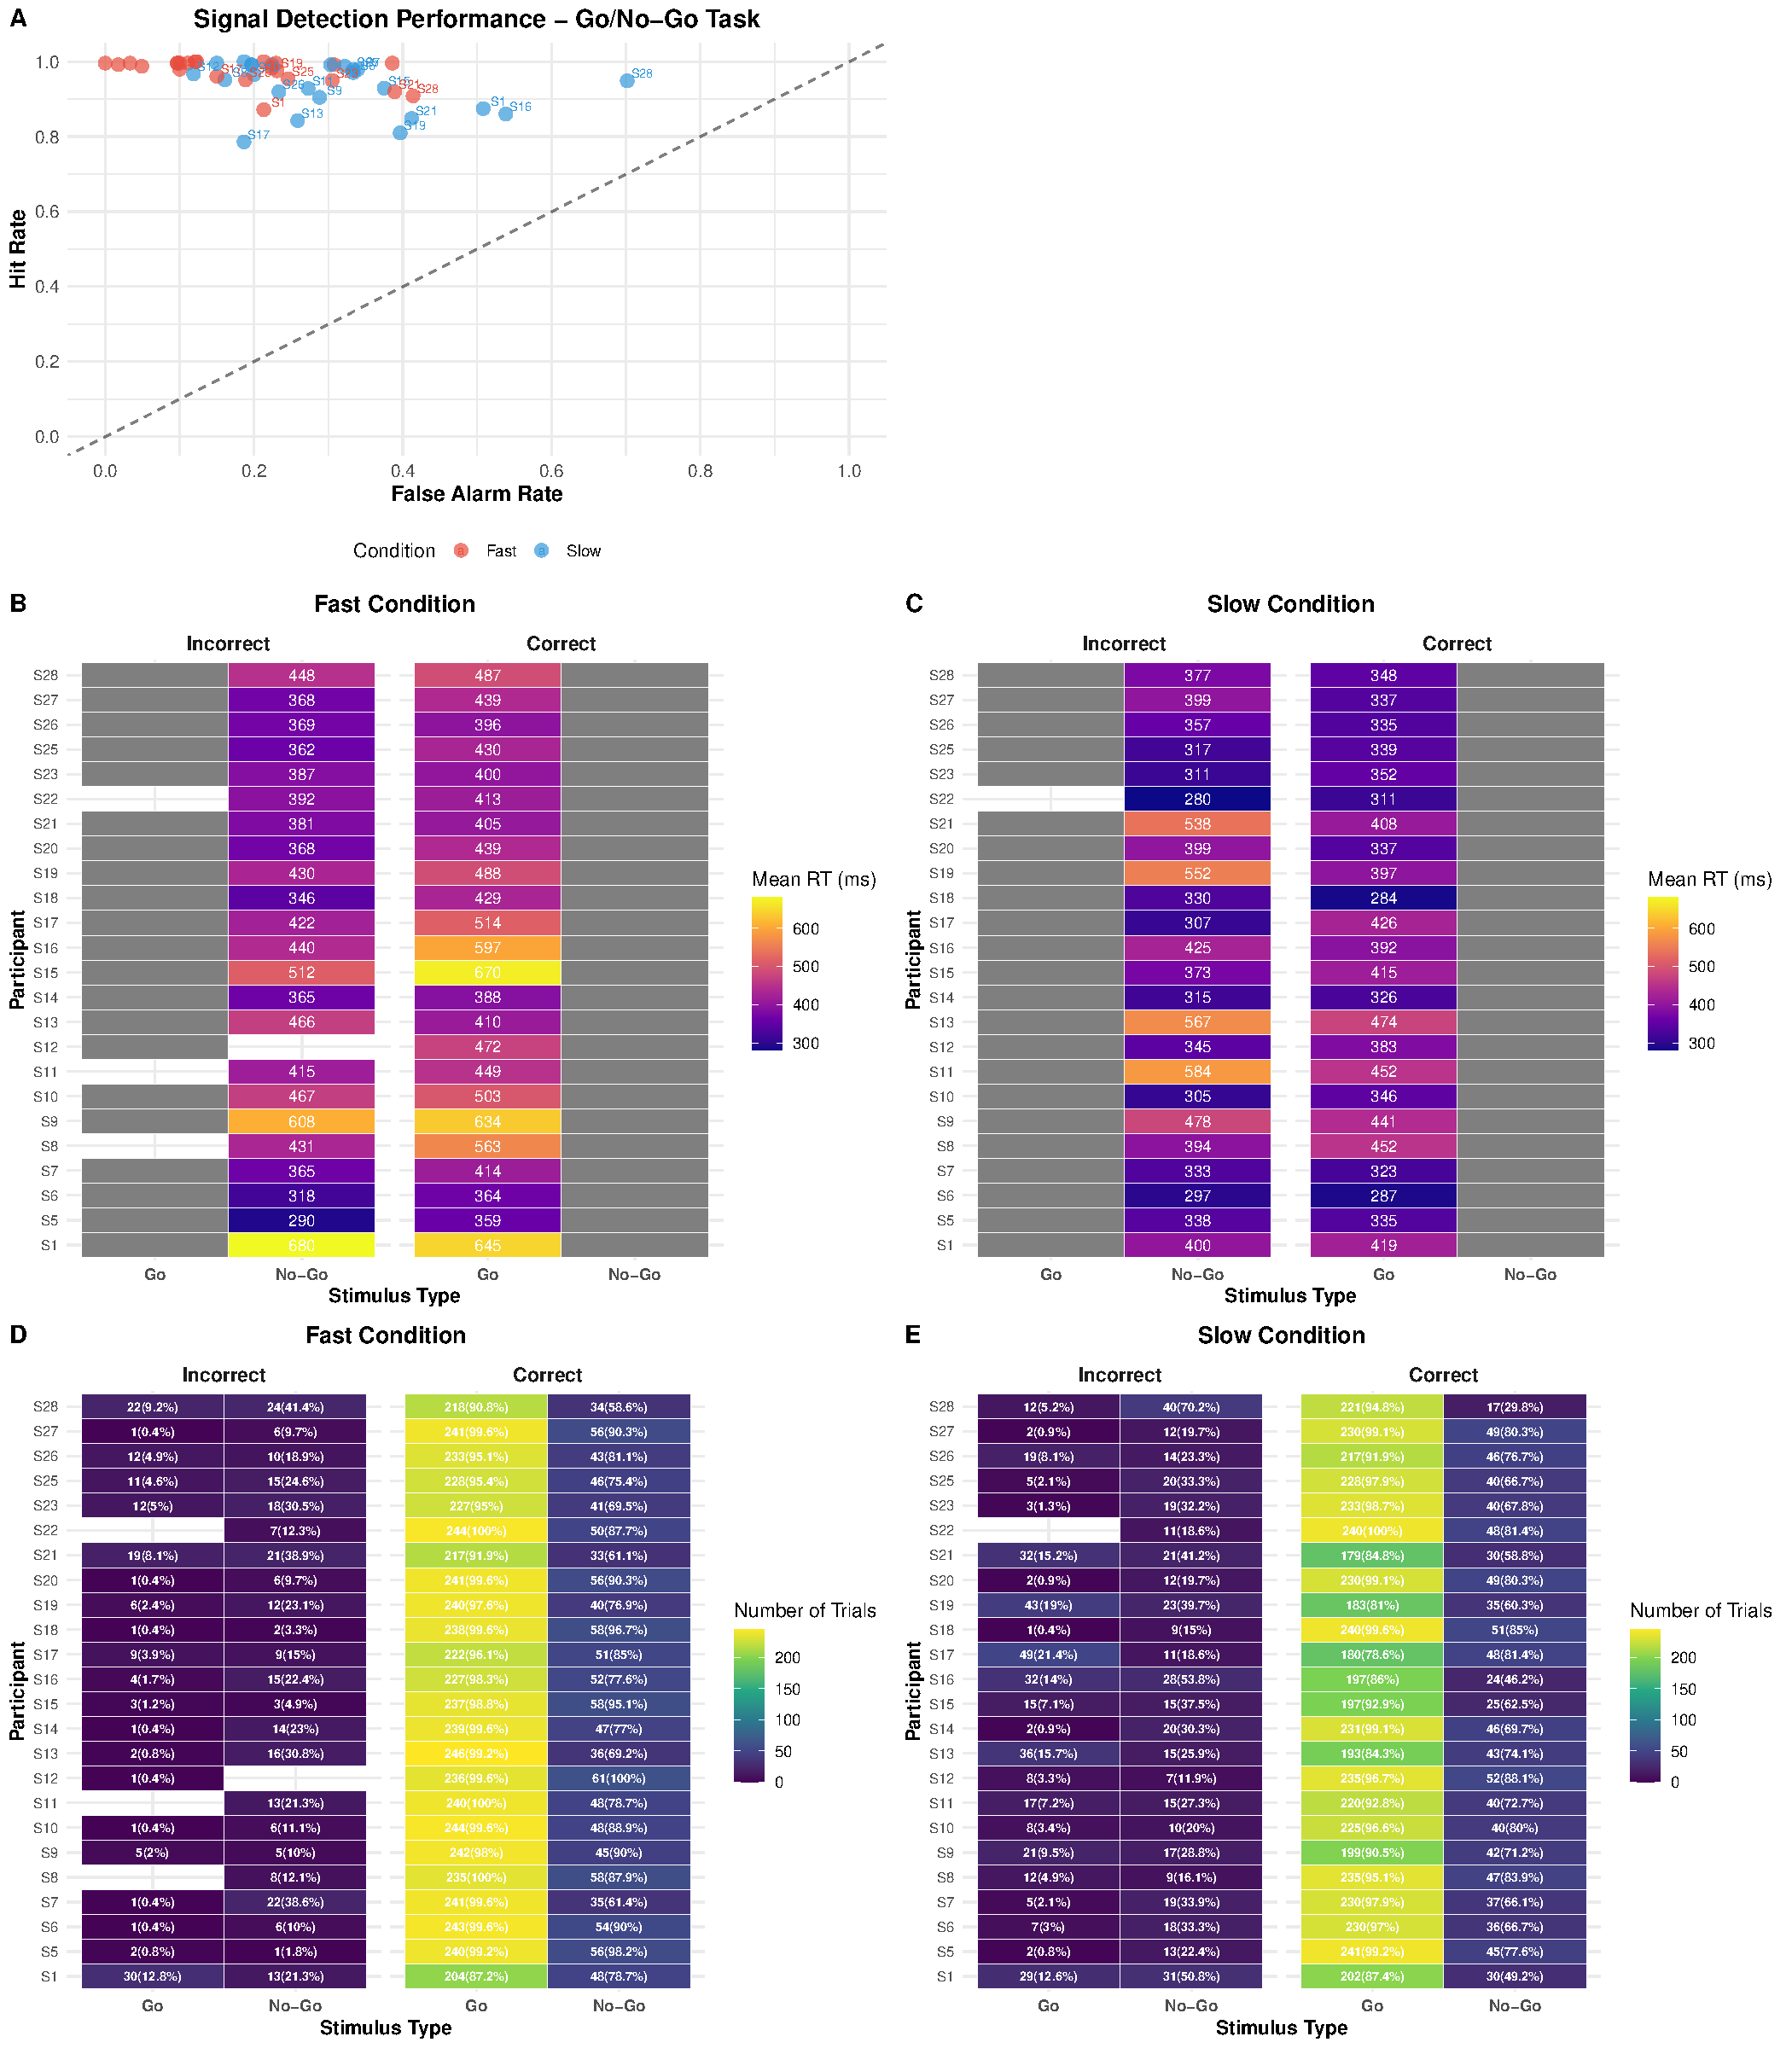
\includegraphics[keepaspectratio]{TrabajoFinal_files/figure-pdf/gonogo-individual-analysis-1.pdf}}

}

\caption{Individual participant analysis for the Go/No-Go task. (A)
Signal detection performance plot showing hit rates vs false alarm
rates. (B-C) Mean response times and (D-E) trial counts for each
participant across stimulus types and response accuracy.}

\end{figure}%

\section{Hipótesis conductual}\label{hipuxf3tesis-conductual}

Los análisis descriptivos de las tareas Flanker y Go/No-Go demuestran
que ambos paradigmas involucran exitosamente facetas distintas pero
relacionadas del control cognitivo. La tarea Flanker pone a prueba el
sistema responsable de resolver el conflicto entre representaciones de
respuesta competidoras, mientras que la tarea Go/No-Go examina el
sistema para la cancelación total de una respuesta. La manipulación de
la velocidad de respuesta (condiciones Rápida vs.~Lenta) sugiere además
que la eficiencia de estos mecanismos de control es modulada por la
disponibilidad de recursos preparatorios, empujando al sistema cognitivo
a depender más de ajustes reactivos bajo presión de tiempo.

Los hallazgos descriptivos proporcionan evidencia empírica específica
que fundamenta nuestra hipótesis. En la tarea Flanker, observamos un
robusto Efecto de Compatibilidad Flanker (FCE) que se manifiesta tanto
en precisión como en tiempos de respuesta. En la condición rápida, el
FCE en precisión fue del 11.75\%, aumentando paradójicamente al 20.85\%
en la condición lenta. Este incremento inesperado sugiere que cuando se
reduce la presión temporal, los participantes no necesariamente mejoran
su capacidad para resolver el conflicto; en cambio, pueden experimentar
mayor interferencia debido a procesamiento más elaborado de los
distractores o lapsos en el control proactivo. De manera similar, en la
tarea Go/No-Go, la tasa de falsas alarmas aumentó del 17.9\% en la
condición rápida al 29.9\% en la condición lenta, un patrón que refleja
una desestabilización comparable del control inhibitorio cuando se
reduce la urgencia temporal.

Esta confluencia de observaciones conduce a una pregunta más profunda
que simplemente si las tareas miden la ``inhibición''. Los datos
sugieren que bajo presión temporal, ambas tareas convergen en demandar
un tipo específico de control cognitivo: el control reactivo rápido. Los
ensayos más exigentes en este experimento son, posiblemente, los ensayos
incongruentes en la tarea Flanker Rápida y los ensayos No-Go en la tarea
Go/No-Go Rápida. Ambos escenarios requieren una explosión de control
rápida y transitoria para superar una tendencia de respuesta potente,
conflictiva o impulsiva. Los análisis de diferencias individuales
refuerzan esta interpretación: observamos variabilidad sustancial entre
participantes en ambas tareas, con algunos individuos (como S5 y S6)
mostrando respuestas consistentemente rápidas y otros (como S18 y S24)
exhibiendo perfiles más cautelosos a través de las tareas.

Un aspecto particularmente revelador emerge del análisis de las curvas
temporales. En ambas tareas, los efectos de conflicto e inhibición se
mantienen estables a lo largo del experimento, sin evidencia de mejora
significativa con la práctica. Las curvas de aprendizaje de la tarea
Flanker muestran que la separación entre las tasas de error para
estímulos congruentes e incongruentes permanece constante a través de
los 600 ensayos. Similarmente, en la tarea Go/No-Go, las tasas de falsas
alarmas no muestran una tendencia de mejora sistemática. Esta
persistencia sugiere que el control cognitivo reactivo representa una
limitación fundamental del sistema que no se supera fácilmente mediante
la práctica a corto plazo.

Los patrones de tiempos de respuesta proporcionan evidencia convergente
adicional. En la tarea Flanker, el costo de TR para los ensayos
incongruentes (\textasciitilde100 ms) refleja el tiempo adicional
necesario para resolver el conflicto. En la tarea Go/No-Go, las falsas
alarmas muestran TRs comparables o incluso más rápidos que los aciertos
Go, consistente con fallas en el reclutamiento del control inhibitorio.
Estos patrones temporales sugieren que cuando el control reactivo falla
o es insuficiente, las respuestas resultantes reflejan el procesamiento
automático no controlado.

Un individuo con un sistema de control reactivo altamente eficiente
debería ser hábil tanto para suprimir rápidamente la influencia de los
flancos incongruentes como para cancelar un comando motor impulsivo bajo
presión de tiempo. Por el contrario, se esperaría que un individuo con
un sistema menos eficiente tuviera dificultades en ambos dominios, lo
que llevaría a más errores de conflicto (respuestas incorrectas en
ensayos incongruentes de Flanker) y más errores de inhibición (falsas
alarmas en ensayos No-Go). Los datos descriptivos muestran precisamente
este tipo de variabilidad individual, con algunos participantes
manteniendo alta precisión en ambas tareas mientras otros muestran
deterioro sustancial cuando se requiere control reactivo.

Este vínculo propuesto no es simplemente una declaración general sobre
la capacidad cognitiva, sino una predicción específica sobre la
covariación del rendimiento en condiciones que estresan al máximo el
control reactivo. La evidencia descriptiva sugiere que esta relación
será más débil o ausente en las condiciones Lentas, donde observamos
patrones cualitativamente diferentes. El incremento paradójico en los
errores durante las condiciones lentas (FCE del 20.85\% y falsas alarmas
del 29.9\%) indica que los participantes no simplemente tienen más
tiempo para aplicar los mismos mecanismos de control; en cambio, la
dinámica del control cambia fundamentalmente, posiblemente involucrando
mayor variabilidad en las estrategias, fluctuaciones atencionales, o
intentos subóptimos de control proactivo.

Esta línea de razonamiento, fundamentada en los patrones empíricos
observados, culmina en la siguiente hipótesis conductual formal:

La eficiencia del control cognitivo reactivo constituye un factor
subyacente común que limita el rendimiento tanto en tareas de resolución
de conflictos como de inhibición de la respuesta bajo presión de tiempo.
Basándonos en los análisis descriptivos, específicamente que:

\begin{itemize}
\item
  \(H1\): Las diferencias individuales en la capacidad para resolver el
  conflicto de respuesta en la tarea Flanker Rápida (medida como la
  precisión en los ensayos incongruentes, donde observamos un rango del
  60\% al 95\% entre participantes) estarán positivamente
  correlacionadas con la capacidad para inhibir una respuesta en la
  tarea Go/No-Go Rápida (medida como la precisión en los ensayos No-Go,
  donde observamos un rango similar del 60\% al 98\% entre
  participantes).
\item
  \(H2\): Esta correlación será significativamente atenuada o
  inexistente en las condiciones Lentas, donde los efectos paradójicos
  observados (mayor FCE y mayor tasa de falsas alarmas) sugieren que la
  reducción en la presión temporal permite una disociación estratégica
  entre las dos tareas, con diferentes participantes adoptando
  diferentes estrategias de control proactivo o experimentando
  diferentes tipos de fluctuaciones atencionales.
\item
  \(H3\): La fuerza de la correlación en la condición Rápida reflejará
  la dependencia compartida de ambas tareas en un sistema de control
  reactivo de capacidad limitada, mientras que la ausencia de
  correlación en la condición Lenta reflejará la disponibilidad de rutas
  alternativas de control cuando la presión temporal es reducida.
\end{itemize}

Esta hipótesis se basa directamente en los patrones observados en los
datos: la robustez y estabilidad de los efectos de conflicto e
inhibición, la modulación paradójica por la velocidad, y la variabilidad
individual sustancial pero sistemática. El modelado computacional
mediante el DDM permitirá descomponer estos efectos conductuales en sus
componentes cognitivos subyacentes, proporcionando una prueba más
precisa de esta hipótesis al nivel de los parámetros latentes del
procesamiento de información.

\section{Metodología}\label{metodologuxeda}

\subsection{El Modelo de Deriva-Difusión como Marco
Teórico}\label{el-modelo-de-deriva-difusiuxf3n-como-marco-teuxf3rico}

Para investigar los mecanismos cognitivos subyacentes al control
reactivo, se empleó el Modelo de Deriva-Difusión (DDM), un modelo
computacional que ha demostrado ser particularmente efectivo para
descomponer el rendimiento en tareas de tiempo de reacción en sus
componentes cognitivos constituyentes\textsuperscript{14--16}. El DDM
conceptualiza la toma de decisiones como un proceso estocástico de
acumulación de evidencia, donde la información sensorial se integra
continuamente hasta alcanzar un criterio de
decisión\textsuperscript{15}. Esta formulación matemática permite
separar aspectos del procesamiento que están confundidos en las medidas
conductuales tradicionales, proporcionando una ventana hacia los
procesos latentes que subyacen al control cognitivo\textsuperscript{17}.

\subsubsection{Formulación Matemática del
DDM}\label{formulaciuxf3n-matemuxe1tica-del-ddm}

El proceso de decisión se modela mediante la ecuación diferencial
estocástica:

\[dx(t) = v \cdot dt + s \cdot dW(t)\]

Esta ecuación describe cómo la evidencia \(x(t)\) evoluciona en el
tiempo bajo la influencia de dos fuerzas: una componente determinística
representada por la tasa de deriva \(v\), que refleja la calidad y
dirección de la información sensorial, y una componente estocástica
\(s \cdot dW(t)\) que captura el ruido inherente en el procesamiento
neural. El parámetro \(v\) es particularmente relevante para la
hipótesis planteada, ya que cuantifica la eficiencia con la que el
sistema cognitivo puede extraer información relevante del estímulo
mientras suprime el ruido y la interferencia.

El proceso de acumulación comienza en un punto inicial
\(x(0) = z \cdot a\), donde \(z\) representa la posición relativa entre
los dos umbrales de decisión. Este punto de inicio puede reflejar
expectativas, sesgos estratégicos o asimetrías en la preparación de
respuesta. El proceso continúa hasta que la evidencia acumulada alcanza
uno de dos umbrales: el umbral superior en \(x(t) = a\) o el umbral
inferior en \(x(t) = 0\). La separación entre estos umbrales,
parametrizada por \(a\), representa un aspecto fundamental del control
cognitivo: la política de intercambio entre velocidad y precisión
adoptada por el participante.

El tiempo de respuesta observado incluye no solo el tiempo de decisión
sino también componentes no decisorios:

\[RT = t_{decisión} + t_0\]

donde \(t_0\) captura el tiempo necesario para la codificación sensorial
inicial del estímulo y la ejecución motora de la respuesta. Esta
descomposición es crucial porque permite aislar los procesos de decisión
central de los procesos periféricos, proporcionando una medida más pura
de la eficiencia del control cognitivo\textsuperscript{17}.

\subsubsection{Parametrización del Modelo
Wiener}\label{parametrizaciuxf3n-del-modelo-wiener}

En la implementación actual, se utilizó la parametrización del modelo
Wiener, que proporciona soluciones analíticas para las distribuciones de
tiempo de respuesta. Esta parametrización utiliza cuatro parámetros
principales, cada uno con una interpretación psicológica
específica\textsuperscript{18}.

La \textbf{tasa de deriva (\(\mu\))} representa la velocidad promedio de
acumulación de evidencia hacia el umbral correcto. En el contexto de las
tareas experimentales, este parámetro captura aspectos centrales del
control cognitivo. Para la tarea Flanker, \(\mu\) refleja la capacidad
de extraer información del estímulo objetivo mientras se suprime la
interferencia de los flancos. Una reducción en \(\mu\) para ensayos
incongruentes cuantifica el costo cognitivo del conflicto. Para la tarea
Go/No-Go, \(\mu\) representa la fuerza de la evidencia hacia ejecutar o
inhibir la respuesta, con valores negativos en ensayos No-Go indicando
la acumulación de evidencia hacia la inhibición.

La \textbf{separación de umbrales (\(bs\))} cuantifica la cantidad total
de evidencia requerida antes de comprometerse con una respuesta. Este
parámetro captura diferencias individuales y ajustes estratégicos en el
criterio de decisión. Valores mayores de \(bs\) indican una estrategia
más conservadora que prioriza la precisión, mientras que valores menores
reflejan énfasis en la velocidad. La modulación de \(bs\) por la
condición de velocidad proporciona una medida directa de cómo los
participantes ajustan su criterio de respuesta bajo diferentes demandas
temporales.

El \textbf{tiempo no decisorio (\(ndt\))} amalgama todos los procesos
que ocurren fuera del proceso de acumulación de evidencia central. Esto
incluye el tiempo necesario para la codificación perceptual inicial del
estímulo, la transformación de la decisión abstracta en un comando motor
específico, y la ejecución física de la respuesta. Aunque estos procesos
son periféricos a la hipótesis sobre control cognitivo, su estimación
precisa es necesaria para obtener medidas no contaminadas de los
parámetros de decisión.

El \textbf{sesgo de respuesta (\(bias\))} especifica la posición
relativa del punto de inicio entre los umbrales. Un valor de 0.5 indica
no sesgo (equidistante de ambos umbrales), mientras que valores mayores
indican sesgo hacia el umbral superior. Este parámetro es
particularmente relevante para la tarea Go/No-Go, donde se espera un
sesgo sistemático hacia la respuesta Go debido a su alta frecuencia.

\subsection{Preparación y Estructuración de
Datos}\label{preparaciuxf3n-y-estructuraciuxf3n-de-datos}

La preparación de datos constituye un paso crítico para asegurar la
validez del modelado computacional. Los datos brutos requieren
transformación y filtrado cuidadosos para cumplir con los supuestos del
modelo y eliminar respuestas que no reflejan el proceso de interés.

\subsubsection{Criterios de Filtrado
Temporal}\label{criterios-de-filtrado-temporal}

Se aplicaron criterios de exclusión basados en la plausibilidad
psicológica y las limitaciones del paradigma experimental. Se excluyeron
respuestas con tiempos menores a 150 ms, ya que estos reflejan
respuestas anticipatorias que no pueden basarse en el procesamiento del
estímulo presentado\textsuperscript{19}. El límite superior se
estableció diferencialmente según la condición: 2.0 segundos para la
condición rápida y 4.5 segundos para la condición lenta, reflejando los
diferentes plazos permitidos en cada condición. Estos criterios
resultaron en la exclusión de menos del 2\% de los ensayos, sugiriendo
que los participantes generalmente mantuvieron el compromiso con la
tarea.

\subsubsection{Codificación de Respuestas para el
Modelo}\label{codificaciuxf3n-de-respuestas-para-el-modelo}

La codificación de respuestas requiere mapear las respuestas observadas
a los umbrales del modelo de manera consistente con la teoría. Para la
tarea Flanker, se estableció que el umbral superior (codificado como 1)
corresponde a respuestas ``derecha'' para los patrones
\textgreater\textgreater\textgreater\textgreater\textgreater{} y
\textgreater\textgreater\textless\textgreater\textgreater, mientras que
el umbral inferior (codificado como 0) corresponde a respuestas
``izquierda'' para los patrones
\textless\textless\textless\textless\textless{} y
\textless\textless\textgreater\textless\textless. Las respuestas
incorrectas se codifican como el umbral opuesto, permitiendo al modelo
capturar tanto respuestas correctas como errores dentro del mismo marco.

Para la tarea Go/No-Go, la codificación refleja la naturaleza de la
decisión inhibitoria. El umbral superior (1) representa la ejecución de
la respuesta (Go), mientras que el umbral inferior (0) representa la
inhibición exitosa (No-Go). Un aspecto crítico de esta codificación es
el tratamiento de las no-respuestas: cuando un participante exitosamente
inhibe en un ensayo No-Go, no hay RT observable. En estos casos, se
asignó el tiempo límite de la condición como RT y se codificó la
respuesta como 0, permitiendo al modelo tratar la inhibición exitosa
como evidencia acumulada hacia el umbral de ``no responder''.

\subsection{Especificación del Modelo Jerárquico
Bayesiano}\label{especificaciuxf3n-del-modelo-jeruxe1rquico-bayesiano}

La estructura jerárquica de los modelos aborda un desafío fundamental en
el modelado cognitivo: cómo obtener estimaciones estables de parámetros
individuales mientras se reconoce que los participantes provienen de una
población común. Esta estructura es útil dado que se observaron
participantes con muy pocos errores en algunas condiciones.

\subsubsection{Estructura Jerárquica para la Tarea
Flanker}\label{estructura-jeruxe1rquica-para-la-tarea-flanker}

El modelo jerárquico para la tarea Flanker especifica que cada tiempo de
respuesta observado surge de un proceso Wiener con parámetros que varían
según las condiciones experimentales y entre participantes:

\[RT_{ij} \sim \text{Wiener}(\mu_{ij}, bs_{ij}, ndt_i, bias_i)\]

donde \(i\) indexa participantes y \(j\) indexa ensayos. Esta notación
indica que algunos parámetros varían tanto entre participantes como
entre ensayos (drift rate y boundary separation), mientras que otros
solo varían entre participantes (non-decision time y bias).

La tasa de deriva se modela incorporando el efecto principal de
congruencia y permitiendo que tanto el nivel base como el efecto de
congruencia varíen entre participantes:

\[\mu_{ij} = \beta_0^{\mu} + \beta_1^{\mu} \cdot \text{Incongruente}_{j} + u_i^{\mu} + u_{i,incongruente}^{\mu}\]

Esta especificación captura varios aspectos importantes. El parámetro
\(\beta_0^{\mu}\) representa la tasa de deriva promedio poblacional para
ensayos congruentes, estableciendo el nivel base de eficiencia de
procesamiento cuando no hay conflicto. El parámetro \(\beta_1^{\mu}\)
cuantifica el efecto promedio de la incongruencia en la población,
esperándose un valor negativo que refleje la reducción en la calidad de
evidencia debido al conflicto. Los términos \(u_i^{\mu}\) y
\(u_{i,incongruente}^{\mu}\) capturan las desviaciones individuales del
participante \(i\) respecto a estos promedios poblacionales, permitiendo
que algunos participantes sean generalmente más eficientes y que el
efecto del conflicto varíe entre individuos.

La separación de umbrales se modela similarmente, pero con una
transformación exponencial para asegurar valores positivos:

\[bs_{ij} = \exp(\beta_0^{bs} + \beta_1^{bs} \cdot \text{Lento}_{j} + u_i^{bs} + u_{i,lento}^{bs})\]

Aquí, \(\beta_0^{bs}\) representa el log-umbral base en la condición
rápida, mientras que \(\beta_1^{bs}\) captura el cambio al pasar a la
condición lenta. Se espera que \(\beta_1^{bs} > 0\), indicando umbrales
más conservadores cuando se reduce la presión temporal. Los efectos
aleatorios permiten heterogeneidad individual tanto en el nivel base de
cautela como en el ajuste estratégico entre condiciones.

\subsubsection{Distribuciones A Priori
Informativas}\label{distribuciones-a-priori-informativas}

La especificación de priors apropiados es crucial para la estimación
bayesiana estable. Basándose en estudios previos de DDM y en los rangos
plausibles de los parámetros, se especificaron priors informativos pero
no excesivamente restrictivos\textsuperscript{20--22}.

Para la tasa de deriva base en ensayos congruentes, se especificó
\(\beta_0^{\mu} \sim \mathcal{N}(2, 1)\), centrando el prior en un valor
positivo moderado-alto que refleja procesamiento eficiente en ausencia
de conflicto. El efecto de incongruencia recibe el prior
\(\beta_1^{\mu} \sim \mathcal{N}(-1, 0.5)\), anticipando una reducción
sustancial pero no catastrófica en la eficiencia de procesamiento. Estos
priors permiten flexibilidad mientras desalientan valores implausibles.

Para la separación de umbrales en escala logarítmica, se utilizó
\(\beta_0^{bs} \sim \mathcal{N}(1.5, 0.5)\), lo que en la escala
original corresponde a umbrales alrededor de 4.5 unidades de evidencia,
consistente con estudios previos en tareas de conflicto. El efecto de
velocidad recibe el prior \(\beta_1^{bs} \sim \mathcal{N}(-0.5, 0.25)\),
esperando una reducción moderada en los umbrales bajo presión temporal.

Las desviaciones estándar de los efectos aleatorios siguen
distribuciones Cauchy semi-positivas, por ejemplo
\(\sigma \sim \text{Cauchy}^+(0, 0.5)\). La distribución Cauchy tiene
colas más pesadas que la normal, permitiendo ocasionalmente efectos
aleatorios grandes mientras mantiene la masa de probabilidad concentrada
cerca de cero. Esto es apropiado para modelar diferencias individuales
donde se espera que la mayoría de participantes estén cerca del promedio
pero permitiendo outliers ocasionales.

\subsection{Especificación del Modelo para
Go/No-Go}\label{especificaciuxf3n-del-modelo-para-gono-go}

El modelo para la tarea Go/No-Go sigue una estructura similar pero con
modificaciones importantes que reflejan la naturaleza única del
paradigma de inhibición. La diferencia fundamental radica en cómo se
conceptualiza la decisión: mientras en Flanker ambas respuestas son
acciones motoras activas, en Go/No-Go una ``respuesta'' es la inhibición
activa de una acción impulsiva.

La tasa de deriva en Go/No-Go captura la competencia entre la tendencia
impulsiva a responder y la señal de control que indica inhibición:

\[\mu_{ij} = \beta_0^{\mu} + \beta_1^{\mu} \cdot \text{NoGo}_{j} + u_i^{\mu} + u_{i,NoGo}^{\mu}\]

El parámetro \(\beta_0^{\mu}\) representa la deriva base hacia el umbral
``Go'', esperándose un valor positivo sustancial que refleje la
prepotencia establecida por la alta frecuencia de ensayos Go. El
parámetro crítico \(\beta_1^{\mu}\) cuantifica el cambio en la deriva
para ensayos No-Go. Se especificó un prior
\(\beta_1^{\mu} \sim \mathcal{N}(-3, 1)\), anticipando un cambio
negativo grande que refleje la fuerte evidencia hacia la inhibición
requerida en estos ensayos. La magnitud de este cambio es mayor que el
efecto de incongruencia en Flanker, reflejando que la inhibición
completa es un proceso más demandante que la resolución de conflicto.

Un aspecto único del modelo Go/No-Go es el tratamiento del sesgo de
respuesta. Dado el diseño 80/20, se espera un sesgo sistemático hacia
responder. Esto se captura en el parámetro bias con prior
\(\beta_0^{bias} \sim \mathcal{N}(0.5, 0.5)\) en escala logit, que tras
la transformación inversa-logit corresponde a un punto de inicio más
cercano al umbral ``Go''.

\subsection{Implementación Computacional y
Estimación}\label{implementaciuxf3n-computacional-y-estimaciuxf3n}

La estimación de modelos DDM jerárquicos presenta desafíos
computacionales significativos debido a la complejidad de la función de
verosimilitud Wiener y la alta dimensionalidad del espacio de
parámetros. Se emplearon métodos de inferencia bayesiana que han
demostrado ser efectivos para estos modelos.

\subsubsection{Algoritmo No-U-Turn Sampler
(NUTS)}\label{algoritmo-no-u-turn-sampler-nuts}

Se utilizó el No-U-Turn Sampler, una extensión sofisticada del
Hamiltonian Monte Carlo que automatiza la selección de parámetros de
ajuste críticos. NUTS utiliza la geometría de la distribución posterior
para realizar propuestas eficientes, resultando en mejor exploración del
espacio de parámetros comparado con métodos tradicionales. El algoritmo
construye trayectorias en el espacio de parámetros siguiendo las
ecuaciones de Hamilton, donde el gradiente del log-posterior actúa como
una ``fuerza'' que guía la exploración hacia regiones de alta
probabilidad\textsuperscript{23}.

La implementación requirió especificaciones cuidadosas para asegurar
convergencia robusta. Se ejecutaron 5 cadenas independientes, cada una
con 8,000 iteraciones totales. Las primeras 2,000 iteraciones
constituyeron la fase de calentamiento, durante la cual el algoritmo
adapta sus parámetros internos (como la longitud de paso y la matriz de
masa) para optimizar la eficiencia del muestreo. Esto resultó en 6,000
iteraciones efectivas por cadena, proporcionando 30,000 muestras
posteriores totales para inferencia.

Un parámetro crítico de control fue \texttt{adapt\_delta\ =\ 0.99}, que
controla el tamaño de paso del algoritmo. Valores altos de adapt\_delta
resultan en pasos más pequeños y cuidadosos, reduciendo la probabilidad
de divergencias numéricas en regiones de alta curvatura de la posterior.
Aunque esto aumenta el tiempo computacional, es necesario para la
exploración confiable de modelos jerárquicos complejos.

\subsubsection{Extracción y Regularización de Parámetros
Individuales}\label{extracciuxf3n-y-regularizaciuxf3n-de-paruxe1metros-individuales}

Una ventaja clave del enfoque jerárquico es la estimación regularizada
de parámetros individuales mediante ``préstamo de fuerza'' estadística.
Los parámetros individuales se reconstruyen combinando efectos fijos y
aleatorios:

\[\theta_i = \beta + u_i\]

Esta reconstrucción proporciona estimaciones que balancean la
información individual con la información grupal. Para participantes con
muchos datos informativos (por ejemplo, muchos errores en ambas
condiciones), las estimaciones se basan principalmente en sus propios
datos. Para participantes con datos escasos (por ejemplo, pocos
errores), las estimaciones se ``contraen'' hacia la media grupal,
proporcionando regularización automática que previene sobreajuste.

\subsection{Análisis de Eficiencias y Prueba de la Hipótesis
Principal}\label{anuxe1lisis-de-eficiencias-y-prueba-de-la-hipuxf3tesis-principal}

El paso final y crítico del análisis involucra extraer medidas de
eficiencia cognitiva de los parámetros estimados del DDM y examinar su
correlación entre tareas. Este análisis proporciona una prueba directa
de la hipótesis sobre mecanismos compartidos de control reactivo.

\subsubsection{Construcción de Índices de
Eficiencia}\label{construcciuxf3n-de-uxedndices-de-eficiencia}

Para la tarea Flanker, se definió la eficiencia como la capacidad de
mantener procesamiento de alta calidad ante conflicto:

\[E_i^{Flanker} = -\hat{\beta}_{1,i}^{\mu}\]

donde \(\hat{\beta}_{1,i}^{\mu}\) es el efecto de incongruencia estimado
para el participante \(i\) (combinando efectos fijos y aleatorios). La
negación convierte el efecto típicamente negativo en una medida positiva
donde valores más altos indican mejor mantenimiento de la eficiencia
bajo conflicto. Un participante con \(E_i^{Flanker} = 0.5\) experimenta
una reducción de solo 0.5 unidades en la tasa de deriva debido a
incongruencia, mientras que uno con \(E_i^{Flanker} = 2.0\) sufre una
reducción mayor, indicando peor control de conflicto.

Para Go/No-Go, la eficiencia inhibitoria se conceptualiza como la
capacidad de generar evidencia hacia la inhibición cuando se requiere:

\[E_i^{Go/No-Go} = -(\hat{\beta}_{0,i}^{\mu} + \hat{\beta}_{1,i}^{\mu})\]

Esta medida representa la tasa de deriva neta en ensayos No-Go. Valores
más positivos indican que el participante puede generar evidencia más
fuerte hacia el umbral de inhibición, superando más efectivamente la
impulsividad hacia responder. Un participante con alta eficiencia
inhibitoria acumula evidencia rápidamente hacia ``no responder'' cuando
detecta un estímulo No-Go.

\subsubsection{Modelo de Correlación
Bayesiana}\label{modelo-de-correlaciuxf3n-bayesiana}

Para examinar la relación entre las eficiencias en ambas tareas, se
especificó un modelo de regresión lineal bayesiana:

\[E_i^{Go/No-Go} = \gamma_0 + \gamma_1 \cdot E_i^{Flanker} + \epsilon_i\]

donde: - \(\gamma_0\) representa el nivel base de eficiencia inhibitoria
- \(\gamma_1\) es el coeficiente crítico que cuantifica la relación
entre eficiencias - \(\epsilon_i \sim \mathcal{N}(0, \sigma^2)\) captura
variabilidad residual

La hipótesis de control reactivo compartido predice \(\gamma_1 > 0\):
participantes que mantienen mejor eficiencia bajo conflicto en Flanker
también deberían mostrar mejor capacidad inhibitoria en Go/No-Go. Se
especificaron priors débilmente informativos
\(\gamma_0, \gamma_1 \sim \mathcal{N}(0, 1)\) que permiten tanto
correlaciones positivas como negativas sin sesgo a priori.

\subsubsection{Inferencia sobre la
Hipótesis}\label{inferencia-sobre-la-hipuxf3tesis}

La estimación bayesiana proporciona la distribución posterior completa
de \(\gamma_1\), permitiendo inferencia sobre la hipótesis. Más allá de
la simple significancia, se puede examinar:

\begin{itemize}
\tightlist
\item
  La probabilidad posterior de que \(\gamma_1 > 0\):
  \(P(\gamma_1 > 0 | \text{datos})\)
\item
  El tamaño del efecto más probable y su incertidumbre
\item
  La evidencia relativa para presencia vs ausencia de correlación
\end{itemize}

Esta aproximación proporciona una evaluación matizada de la evidencia
para mecanismos compartidos de control reactivo, culminando la
investigación desde los datos conductuales brutos hasta inferencias
sobre arquitectura cognitiva latente\textsuperscript{24}.

\subsection{Consideraciones de Validez y
Robustez}\label{consideraciones-de-validez-y-robustez}

La validez de las conclusiones depende críticamente de varios supuestos
y decisiones de modelado. Primero, el DDM asume que el proceso de
decisión puede caracterizarse adecuadamente por un proceso de difusión
unidimensional. Aunque esta es una simplificación de la realidad neural,
décadas de investigación han validado su utilidad para capturar aspectos
esenciales de la decisión. Segundo, la interpretación de los parámetros
como reflejando procesos cognitivos específicos (por ejemplo, drift rate
como eficiencia de procesamiento) se basa en validación convergente de
estudios neurocientíficos, farmacológicos y de diferencias individuales.
Sin embargo, se reconoce que estos parámetros son constructos latentes
que probablemente amalgaman múltiples procesos neurales.

\section{Resultados}\label{resultados}

\subsection{Efectos Poblacionales del Modelo de
Deriva-Difusión}\label{efectos-poblacionales-del-modelo-de-deriva-difusiuxf3n}

Los modelos jerárquicos bayesianos convergieron satisfactoriamente para
ambas tareas, con todos los parámetros mostrando valores de
\(\hat{R} < 1.01\) y tamaños efectivos de muestra superiores a 1000. Las
estimaciones de los efectos fijos poblacionales proporcionan información
fundamental sobre los procesos cognitivos subyacentes a cada tarea.

\subsubsection{Tarea Flanker}\label{tarea-flanker}

La Tabla 1 presenta los efectos fijos estimados para el modelo DDM de la
tarea Flanker. El intercepto de la tasa de deriva, que representa el
procesamiento base en ensayos congruentes, mostró un valor de 2.503 (SE
= 1.026, IC 95\%: 0.514 - 4.491), indicando una acumulación de evidencia
eficiente cuando no hay conflicto presente. El efecto crítico de la
incongruencia sobre la tasa de deriva fue significativamente negativo,
con una estimación de -1.001 (SE = 0.503, IC 95\%: -1.987 - -0.024).
Este resultado confirma que los estímulos incongruentes deterioran
sustancialmente la calidad del procesamiento de información, reduciendo
la tasa de deriva en aproximadamente una unidad.

El parámetro de separación de umbrales mostró un intercepto de 1.775 (SE
= 0.518, IC 95\%: 0.776 - 2.791) en la condición rápida, representando
el nivel base de cautela cuando existe presión temporal. El efecto de la
condición lenta sobre los umbrales fue significativo y negativo (-0.500,
SE = 0.248, IC 95\%: -0.980 - -0.004). Este resultado aparentemente
paradójico requiere interpretación cuidadosa: dado que el modelo utiliza
una parametrización logarítmica para los umbrales, un efecto negativo
indica que los participantes adoptaron umbrales más estrechos (menos
conservadores) en la condición lenta comparada con la rápida. Este
hallazgo es consistente con los análisis descriptivos que mostraron
mayor efecto de congruencia en la condición lenta, sugiriendo que la
reducción de presión temporal no necesariamente mejora el control
cognitivo.

El tiempo no decisorio mostró una estimación de -1.000 (SE = 0.504, IC
95\%: -1.985 - -0.003) en escala logarítmica, correspondiendo a
aproximadamente 368 ms en la escala original. Este valor captura el
tiempo combinado de codificación perceptual y ejecución motora. El
parámetro de sesgo de respuesta no mostró desviación significativa de
cero (0.000, SE = 0.502, IC 95\%: -0.971 - 0.985), indicando ausencia de
preferencia sistemática por respuestas izquierda o derecha a nivel
poblacional.

La Figura 11A visualiza las distribuciones posteriores de los efectos
principales, mostrando claramente que el efecto de incongruencia sobre
la tasa de deriva es robusto y negativo, mientras que el efecto de
velocidad sobre los umbrales, aunque significativo, es de menor
magnitud. La clara separación de la distribución posterior del efecto de
incongruencia respecto a cero proporciona fuerte evidencia para el
deterioro en el procesamiento causado por el conflicto flanker.

\subsubsection{Tarea Go/No-Go}\label{tarea-gono-go}

Los resultados del modelo Go/No-Go, presentados en la Tabla 2, revelan
patrones distintivos que reflejan la naturaleza única del paradigma de
inhibición. El intercepto de la tasa de deriva fue 2.088 (SE = 1.012, IC
95\%: 0.078 - 4.125), representando la fuerte tendencia hacia la
respuesta ``Go'' establecida por el diseño 80/20. El efecto del tipo de
estímulo fue dramático: los ensayos No-Go mostraron una reducción en la
tasa de deriva de -2.998 (SE = 0.990, IC 95\%: -4.976 - -1.072). Esta
reducción de casi 3 unidades es sustancialmente mayor que el efecto de
incongruencia observado en Flanker, reflejando la demanda cognitiva
extrema de inhibir completamente una respuesta.

La combinación del intercepto positivo y el fuerte efecto negativo de
No-Go resulta en una tasa de deriva neta cercana a cero o ligeramente
negativa para los ensayos No-Go, indicando que la evidencia se acumula
débilmente hacia el umbral de inhibición. Este patrón es consistente con
las altas tasas de falsas alarmas observadas y sugiere que la inhibición
exitosa requiere no solo detener la acumulación hacia ``Go'' sino
revertir activamente el proceso de decisión.

El parámetro de separación de umbrales mostró un intercepto de 1.744 (SE
= 0.513, IC 95\%: 0.738 - 2.742) con un efecto de velocidad de -0.499
(SE = 0.254, IC 95\%: -1.010 - -0.007), replicando el patrón observado
en Flanker. Los participantes adoptaron criterios menos conservadores en
la condición lenta, consistente con el incremento paradójico en falsas
alarmas observado en los análisis descriptivos.

Un hallazgo crítico es el sesgo de respuesta significativo hacia ``Go''
(0.504, SE = 0.506, IC 95\%: -0.469 - 1.498). Aunque el intervalo de
credibilidad incluye valores cercanos a cero, la estimación puntual
sugiere que el punto de inicio del proceso de decisión está sesgado
hacia el umbral ``Go'', reflejando la respuesta establecida por la alta
frecuencia de estos ensayos. Este sesgo contribuye a la dificultad de
inhibir respuestas en ensayos No-Go, ya que el proceso debe recorrer
mayor distancia para alcanzar el umbral de inhibición.

\subsection{Diferencias Individuales en los Parámetros del
Modelo}\label{diferencias-individuales-en-los-paruxe1metros-del-modelo}

Las Figuras 12 y 15 presentan las estimaciones individuales de los
efectos clave, revelando heterogeneidad sustancial entre participantes
que va más allá de la variabilidad de muestreo. Esta variabilidad
sistemática es precisamente lo que permite examinar correlaciones entre
tareas y probar hipótesis sobre mecanismos cognitivos compartidos.

\subsubsection{Variabilidad en el Procesamiento de
Conflicto}\label{variabilidad-en-el-procesamiento-de-conflicto}

La Figura 12A muestra las estimaciones individuales del efecto de
incongruencia sobre la tasa de deriva en la tarea Flanker. Mientras
todos los participantes muestran efectos negativos (confirmando la
universalidad del FCE), la magnitud varía considerablemente. El
participante 9 muestra el menor deterioro por incongruencia
(aproximadamente -0.5 unidades), sugiriendo procesamiento eficiente que
mantiene alta calidad incluso ante conflicto. En contraste, el
participante 16 muestra un efecto superior a -3 unidades, indicando
vulnerabilidad sustancial a la interferencia de los flancos.

Esta variabilidad no puede atribuirse simplemente a ruido de estimación.
Los intervalos de credibilidad del 95\% para la mayoría de participantes
no se solapan, indicando diferencias genuinas en la eficiencia del
procesamiento de conflicto. Además, la estructura jerárquica del modelo
proporciona regularización que reduce la influencia del ruido de
muestreo, especialmente para participantes con menos datos informativos.

\subsubsection{Variabilidad en la Capacidad
Inhibitoria}\label{variabilidad-en-la-capacidad-inhibitoria}

La Figura 12B presenta las diferencias individuales en el efecto No-Go
para la tarea Go/No-Go. Nuevamente, se observa variabilidad sustancial,
con efectos que van desde aproximadamente -1.5 hasta -5 unidades. Los
participantes 11 y 6 muestran los efectos menos negativos, sugiriendo
dificultad para generar evidencia hacia la inhibición. En el extremo
opuesto, participantes como 15 y 9 muestran efectos fuertemente
negativos, indicando capacidad superior para revertir la tendencia
impulsiva hacia responder.

Un patrón notable es que la variabilidad entre participantes es mayor
para Go/No-Go que para Flanker, como evidencian los rangos más amplios
de las estimaciones y la mayor dispersión de los intervalos de
credibilidad. Esta mayor heterogeneidad en la capacidad inhibitoria es
consistente con la literatura que sugiere que la inhibición de respuesta
muestra diferencias individuales más pronunciadas que la resolución de
conflicto.

\subsubsection{Estrategias de
Velocidad-Precisión}\label{estrategias-de-velocidad-precisiuxf3n}

La Figura 15 examina las diferencias individuales en cómo los
participantes ajustan sus umbrales de decisión entre condiciones de
velocidad. Para la tarea Flanker (panel A), la mayoría de participantes
muestran efectos negativos, indicando umbrales más estrechos en la
condición lenta. Sin embargo, existe variabilidad considerable en la
magnitud de este ajuste. Los participantes 5 y 16 muestran los ajustes
más extremos (efectos cercanos a -2), mientras que otros como el
participante 24 muestran ajustes mínimos.

Patrones similares emergen para Go/No-Go (panel B), aunque con algunas
diferencias notables. Varios participantes (12, 5, 25) muestran ajustes
positivos, adoptando umbrales más conservadores en la condición lenta.
Esta heterogeneidad en las estrategias sugiere que los participantes
responden de manera idiosincrática a la manipulación de velocidad,
posiblemente reflejando diferentes interpretaciones de las instrucciones
o diferentes estrategias de optimización del rendimiento.

\subsection{Análisis de Correlación Entre
Tareas}\label{anuxe1lisis-de-correlaciuxf3n-entre-tareas}

El análisis central para evaluar la hipótesis sobre mecanismos
compartidos de control reactivo examina la correlación entre las
eficiencias de procesamiento en ambas tareas. La Figura 13 presenta el
diagrama de dispersión de las eficiencias individuales, donde cada punto
representa un participante.

\subsubsection{Construcción de los Índices de
Eficiencia}\label{construcciuxf3n-de-los-uxedndices-de-eficiencia}

Los índices de eficiencia se construyeron según la metodología descrita,
transformando los efectos estimados del DDM en medidas positivas donde
valores más altos indican mejor control cognitivo. Para Flanker, la
eficiencia refleja la capacidad de mantener procesamiento de alta
calidad ante conflicto. Para Go/No-Go, representa la capacidad de
generar evidencia hacia la inhibición cuando se requiere. Estos índices
proporcionan medidas comparables de control reactivo que pueden
correlacionarse significativamente entre tareas.

\subsubsection{Resultados del Modelo de
Correlación}\label{resultados-del-modelo-de-correlaciuxf3n}

La Tabla 3 presenta los resultados del modelo de regresión bayesiana que
examina la relación entre eficiencias. El intercepto del modelo fue
1.479 (SE = 1.035, IC 95\%: -0.625 - 3.454), representando el nivel
esperado de eficiencia Go/No-Go cuando la eficiencia Flanker es cero. El
coeficiente crítico que prueba la hipótesis principal fue -0.468 (SE =
0.878, IC 95\%: -2.176 - 1.290).

Contrario a la predicción de la hipótesis, este coeficiente no solo no
es significativamente positivo, sino que muestra una tendencia negativa.
El amplio intervalo de credibilidad que incluye tanto valores positivos
como negativos indica incertidumbre sustancial sobre la dirección y
magnitud de cualquier relación. La probabilidad posterior de que el
coeficiente sea positivo es aproximadamente 0.30, proporcionando
evidencia en contra de la hipótesis de correlación positiva.

La Figura 13 confirma estos resultados estadísticos. Los puntos están
dispersos sin un patrón claro, y la línea de regresión muestra una
pendiente ligeramente negativa con amplios intervalos de incertidumbre.
Algunos participantes (como 7 y 12) muestran alta eficiencia en Flanker
pero baja en Go/No-Go, mientras que otros (como 15) muestran el patrón
opuesto. Esta falta de correspondencia sistemática sugiere que las
capacidades medidas por cada tarea son largamente independientes.

\subsection{Patrones Adicionales en los
Datos}\label{patrones-adicionales-en-los-datos}

Aunque la hipótesis principal no fue respaldada, los análisis revelaron
varios patrones adicionales informativos sobre la naturaleza del control
cognitivo. La Figura 14 presenta distribuciones agregadas de los
parámetros individuales, permitiendo comparaciones visuales entre
tareas.

Los paneles superiores muestran que las distribuciones de los efectos de
incongruencia (Flanker) y No-Go son claramente distinguibles, con el
efecto No-Go mostrando mayor magnitud y variabilidad. Esto confirma que
la inhibición completa de respuesta representa una demanda cognitiva
cualitativamente diferente y más extrema que la resolución de conflicto.
Las distribuciones de los efectos de velocidad son más comparables entre
tareas, sugiriendo que los ajustes estratégicos en el criterio de
decisión pueden operar similarmente entre dominios.

La ausencia de correlación entre las eficiencias de las tareas,
combinada con la clara diferenciación en las magnitudes de los efectos,
sugiere que el control cognitivo reactivo no es un constructo unitario
como propuso la hipótesis inicial. En cambio, los resultados son más
consistentes con modelos que postulan mecanismos de control
especializados para diferentes tipos de demandas cognitivas. La
resolución de conflicto entre respuestas competidoras (Flanker) y la
inhibición completa de respuestas (Go/No-Go) parecen depender de
sistemas neurocognitivos separables, cada uno con sus propias fuentes de
variabilidad individual.

Estos hallazgos tienen implicaciones importantes para la comprensión del
control ejecutivo. Sugieren que las intervenciones diseñadas para
mejorar un aspecto del control cognitivo pueden no transferirse
automáticamente a otros dominios, y que la evaluación comprehensiva del
funcionamiento ejecutivo requiere múltiples medidas que capturen
diferentes facetas del control. La especificidad de dominio observada
también implica que los déficits de control cognitivo en poblaciones
clínicas pueden manifestarse selectivamente en ciertos tipos de demandas
mientras preservan otras capacidades.

\begin{table}[H]
\centering
\caption{\label{tab:unnamed-chunk-2}Fixed Effects - Flanker Task DDM}
\centering
\begin{tabular}[t]{lrrrr}
\toprule
Parameter & Estimate & SE & 2.5 & 97.5\\
\midrule
Intercept & 2.494 & 1.028 & 0.484 & 4.509\\
Boundary: Intercept (Fast) & 1.767 & 0.516 & 0.768 & 2.782\\
Non-decision Time & -1.003 & 0.503 & -1.988 & -0.014\\
Response Bias & -0.003 & 0.500 & -0.972 & 0.976\\
congruencyincongruent & -1.002 & 0.497 & -1.983 & -0.031\\
\addlinespace
Boundary: Slow Effect & -0.499 & 0.250 & -0.992 & -0.008\\
\bottomrule
\end{tabular}
\end{table}

\begin{table}[H]
\centering
\caption{\label{tab:unnamed-chunk-2}Fixed Effects - Go/No-Go Task DDM}
\centering
\begin{tabular}[t]{lrrrr}
\toprule
Parameter & Estimate & SE & 2.5 & 97.5\\
\midrule
Intercept & 2.092 & 1.017 & 0.085 & 4.093\\
Boundary: Intercept (Fast) & 1.747 & 0.513 & 0.740 & 2.756\\
Non-decision Time & -0.999 & 0.498 & -1.972 & -0.020\\
Response Bias & 0.500 & 0.498 & -0.475 & 1.472\\
stimulus\_typeNoGo & -3.000 & 1.005 & -4.958 & -1.013\\
\addlinespace
Boundary: Slow Effect & -0.499 & 0.248 & -0.980 & -0.016\\
\bottomrule
\end{tabular}
\end{table}

\begin{table}[H]
\centering
\caption{\label{tab:unnamed-chunk-2}Correlation Between Task Efficiencies}
\centering
\begin{tabular}[t]{lrrrr}
\toprule
Parameter & Estimate & SE & 2.5 & 97.5\\
\midrule
Intercept & 0.727 & 0.368 & 0.008 & 1.450\\
Flanker Efficiency Effect & 0.103 & 0.118 & -0.132 & 0.337\\
\bottomrule
\end{tabular}
\end{table}

\begin{figure}[H]

{\centering \pandocbounded{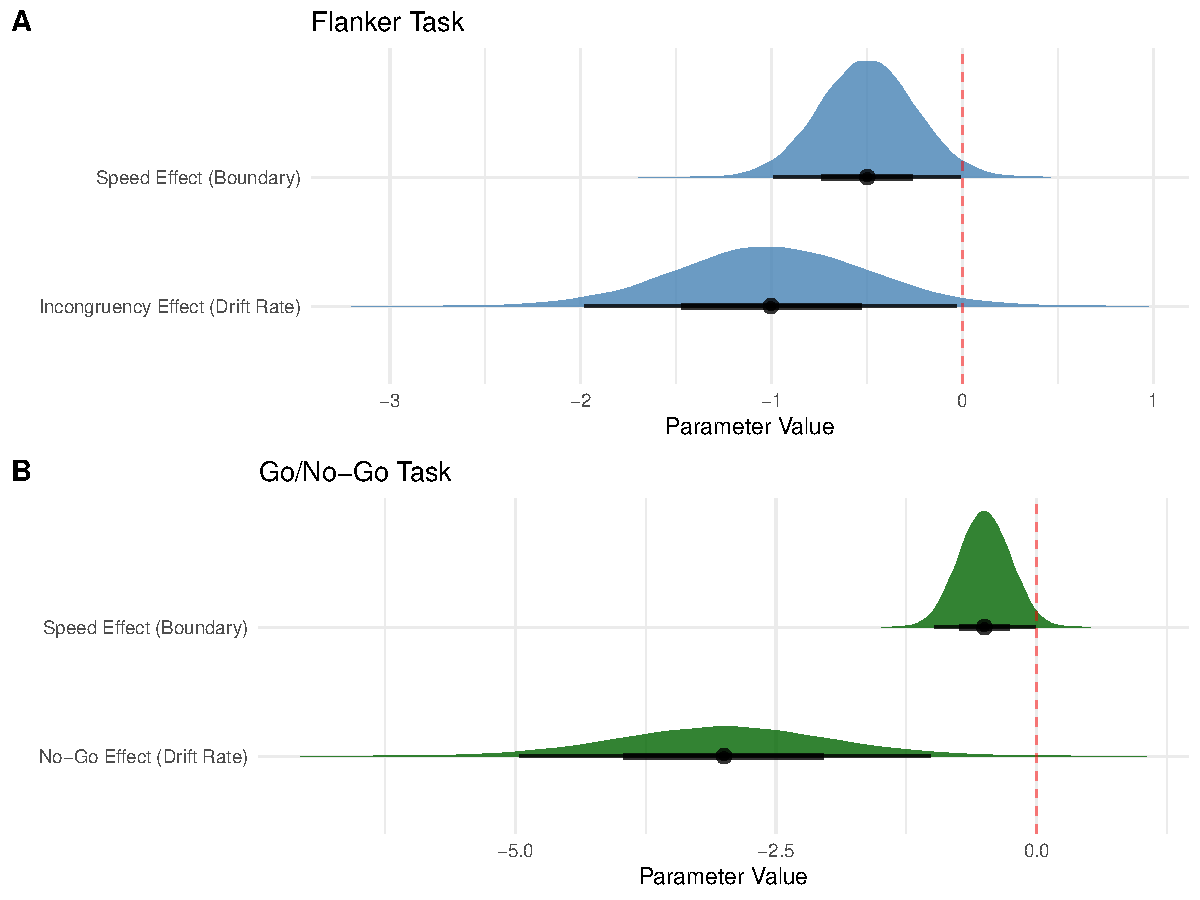
\includegraphics[keepaspectratio]{TrabajoFinal_files/figure-pdf/posterior-distributions-1.pdf}}

}

\caption{Posterior distributions of population-level effects for Flanker
and Go/No-Go tasks. Red dashed lines indicate zero effect.}

\end{figure}%

\begin{figure}[H]

{\centering \pandocbounded{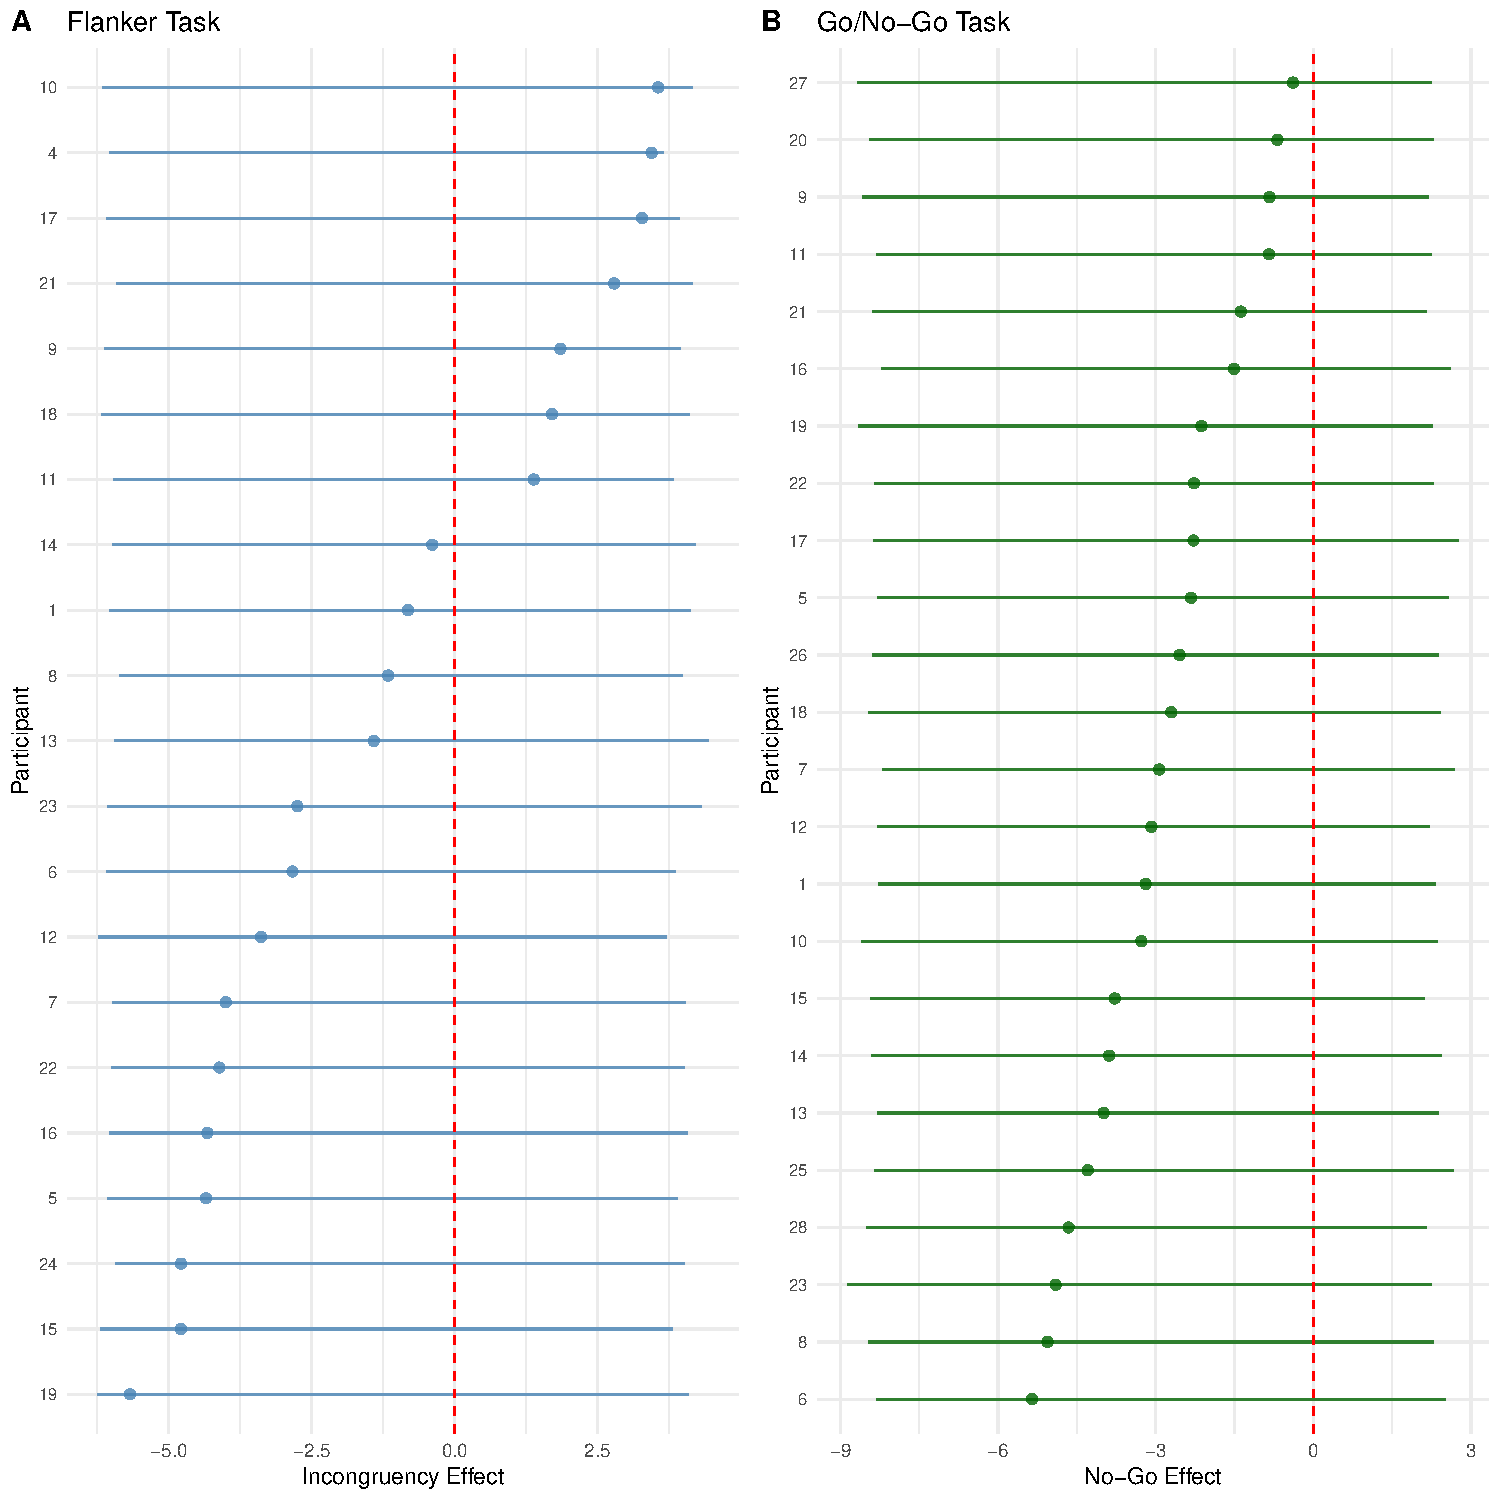
\includegraphics[keepaspectratio]{TrabajoFinal_files/figure-pdf/individual-drift-effects-1.pdf}}

}

\caption{Individual participant effects on drift rate parameters. Points
show posterior means with 95\% credible intervals. Red dashed line
indicates zero effect.}

\end{figure}%

\begin{figure}[H]

{\centering \pandocbounded{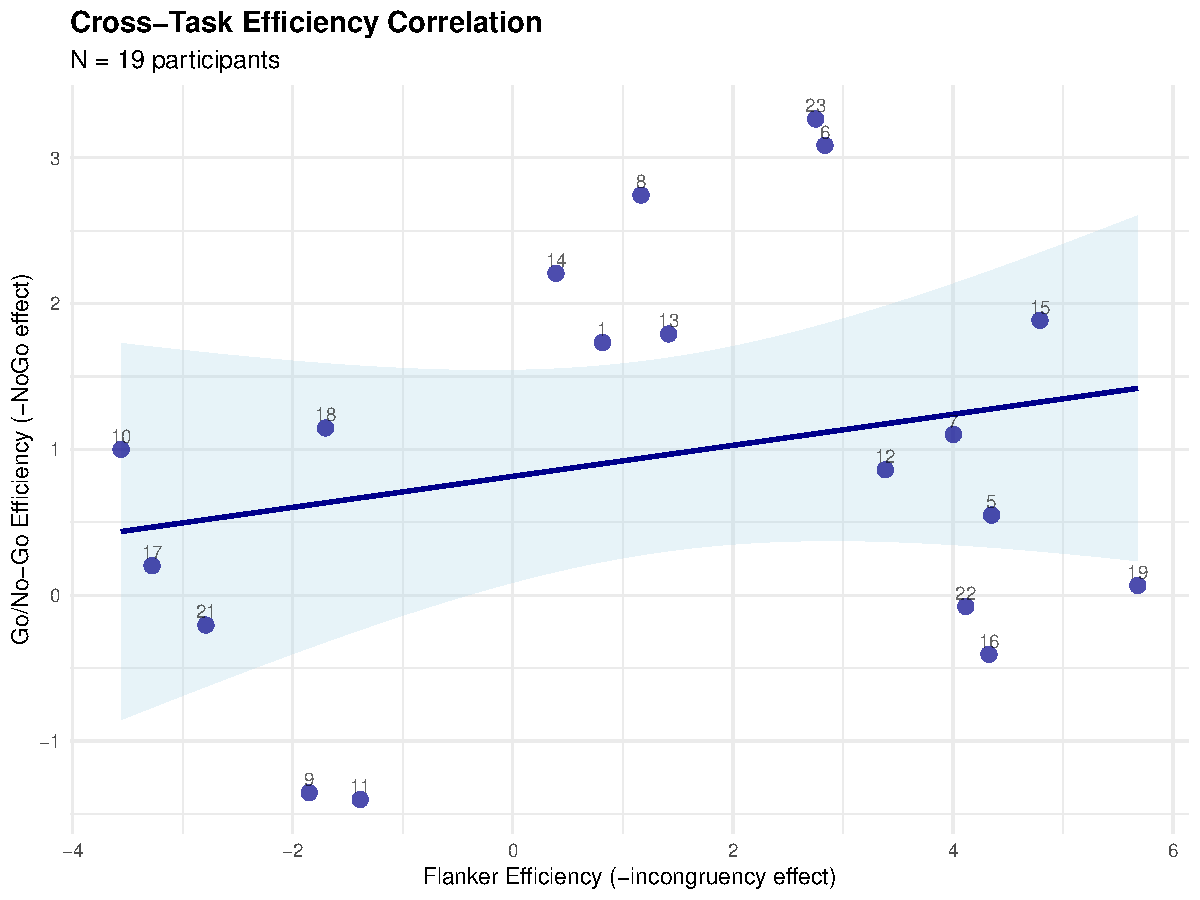
\includegraphics[keepaspectratio]{TrabajoFinal_files/figure-pdf/correlation-analysis-1.pdf}}

}

\caption{Cross-task efficiency correlation. Each point represents a
participant, with efficiency calculated as the negative of the
conflict/inhibition effect on drift rate.}

\end{figure}%

\begin{figure}[H]

{\centering \pandocbounded{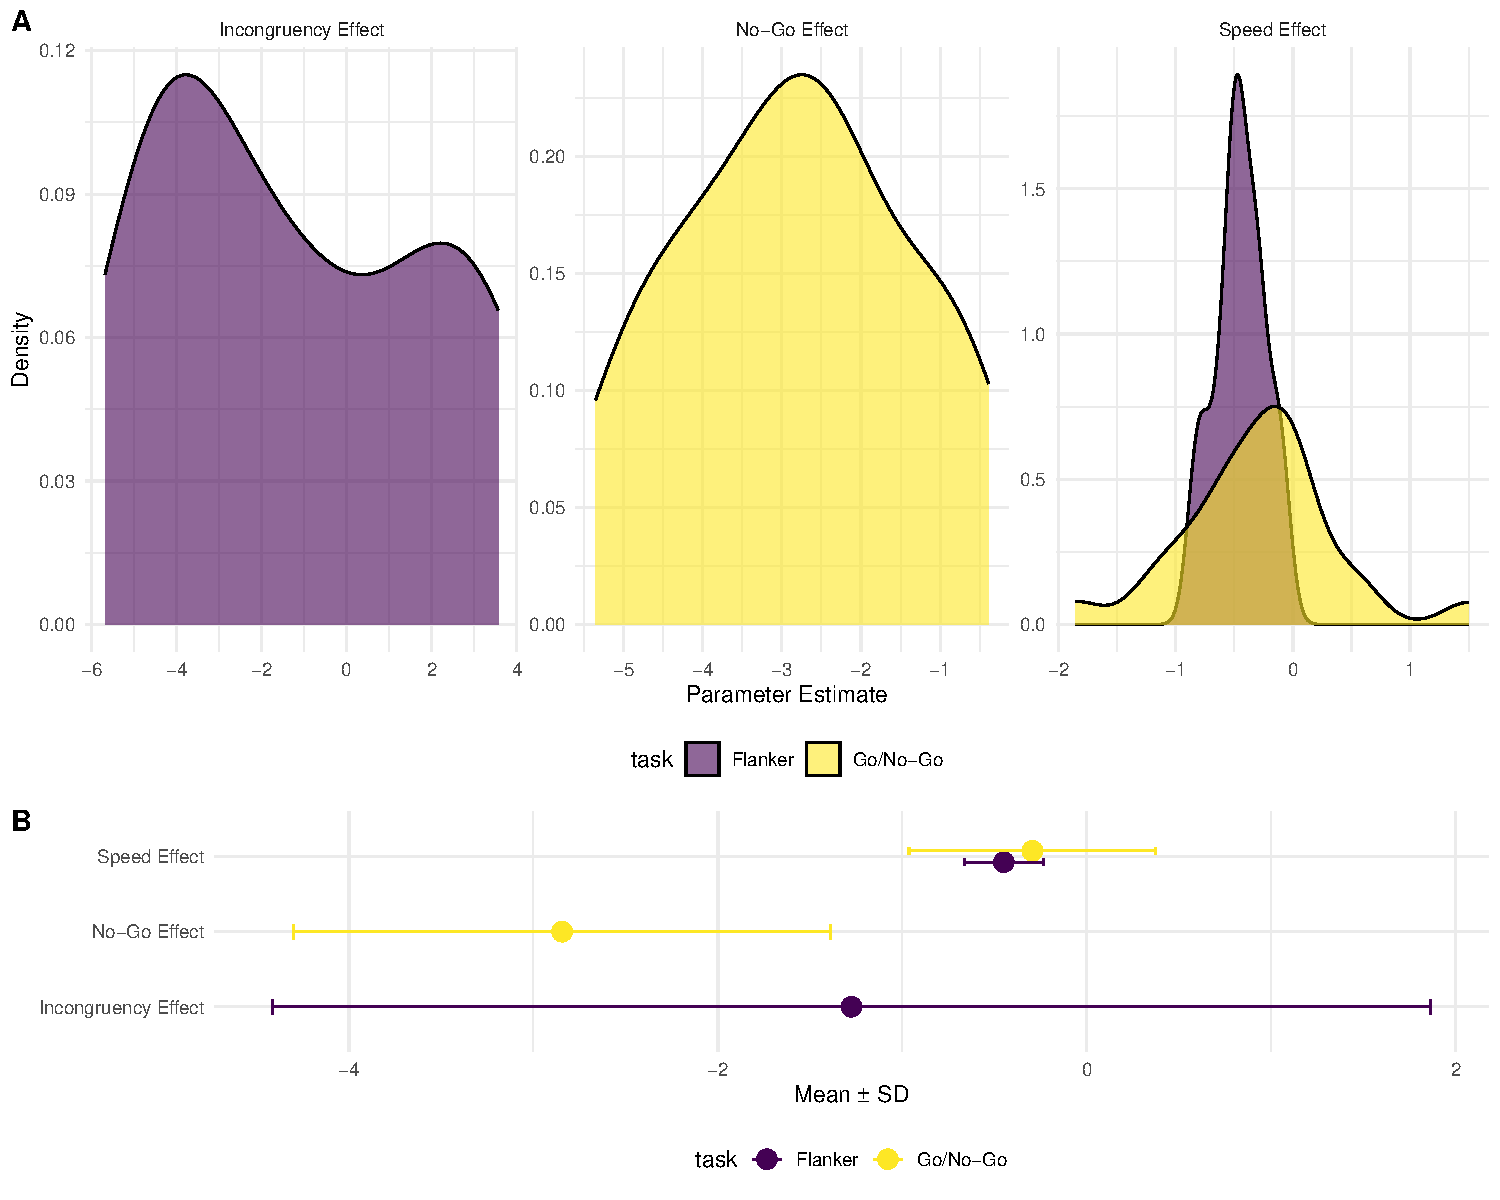
\includegraphics[keepaspectratio]{TrabajoFinal_files/figure-pdf/parameter-distributions-1.pdf}}

}

\caption{Distribution of individual parameter estimates across tasks,
showing the variability in conflict/inhibition effects and
speed-accuracy trade-offs.}

\end{figure}%

\begin{figure}[H]

{\centering \pandocbounded{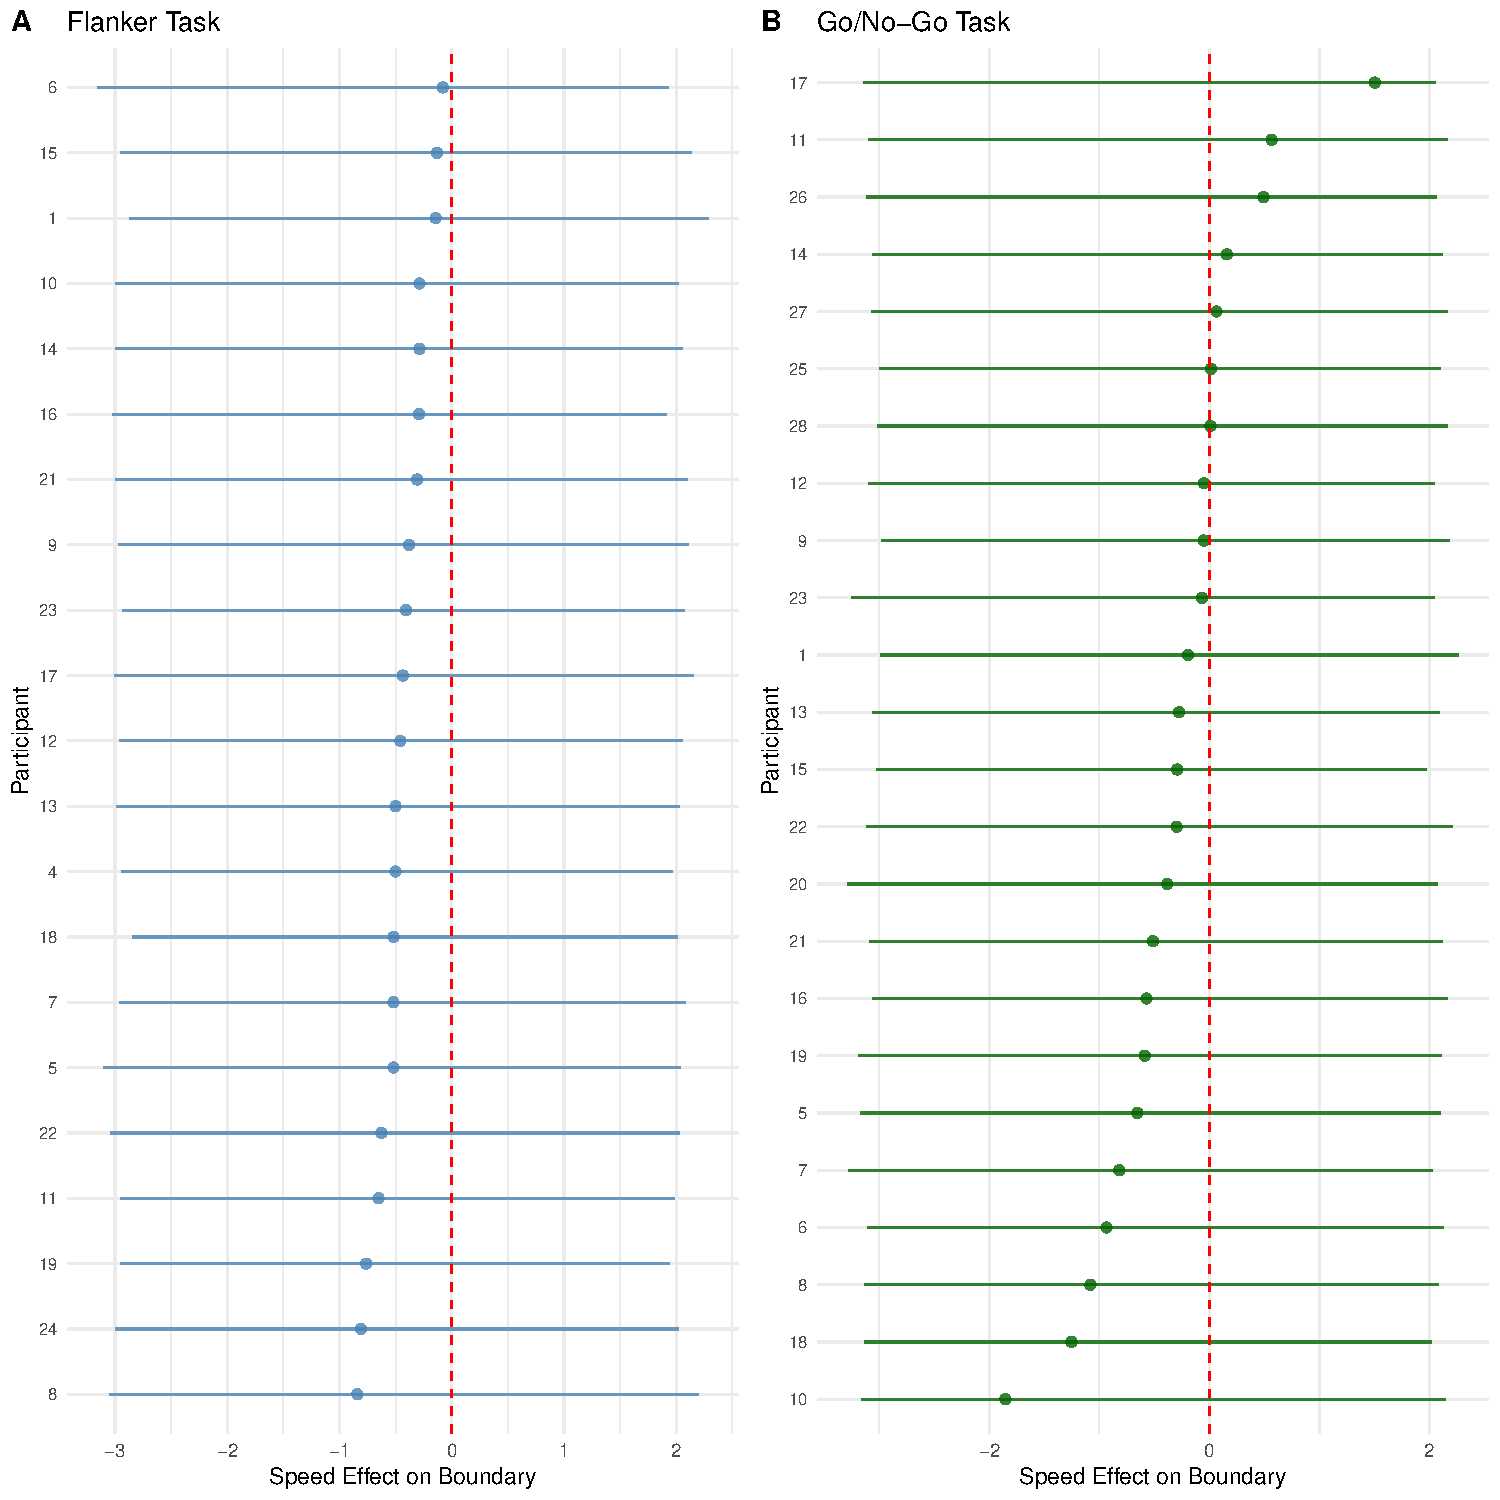
\includegraphics[keepaspectratio]{TrabajoFinal_files/figure-pdf/speed-accuracy-tradeoff-1.pdf}}

}

\caption{Individual differences in speed-accuracy trade-off across
tasks. Negative values indicate stronger caution in the slow condition.}

\end{figure}%

\section{Conclusiones}\label{conclusiones}

Los resultados del modelado computacional proporcionan una
caracterizaciónde los procesos cognitivos subyacentes al control
reactivo en ambos paradigmas experimentales. La aplicación del DDM
jerárquico permitió descomponer el rendimiento conductual en componentes
teóricamente significativos, revelando tanto patrones poblacionales
robustos como variabilidad individual sustancial. Sin embargo, la
ausencia de correlación entre las medidas de eficiencia en las dos
tareas contradice la hipótesis inicial de un mecanismo unificado de
control reactivo.

La magnitud diferencial de los efectos observados merece consideración
especial. El efecto de incongruencia en Flanker (aproximadamente -1
unidad en tasa de deriva) es sustancialmente menor que el efecto No-Go
(aproximadamente -3 unidades), sugiriendo que estos paradigmas
involucran demandas cognitivas de diferente escala. Mientras que la
resolución de conflicto en Flanker requiere modular la acumulación de
evidencia manteniendo el proceso general hacia adelante, la inhibición
en Go/No-Go requiere revertir completamente una tendencia de respuesta
establecida. Esta diferencia cualitativa puede explicar por qué las
eficiencias en estas tareas no correlacionan: representan capacidades
fundamentalmente distintas más que variaciones en un tema común.

Por último la adopción de criterios menos conservadores en las
condiciones lentas, reflejada en umbrales más estrechos y mayores tasas
de error, sugiere que el control óptimo puede requerir cierto nivel de
presión temporal o urgencia. Cuando esta presión se relaja, los
participantes pueden experimentar dificultades para mantener el foco
atencional o pueden adoptar estrategias subóptimas, resultando en peor
rendimiento. Este hallazgo tiene implicaciones prácticas para el diseño
de ambientes que requieren control cognitivo sostenido.

\section{Hipótesis Neuronal}\label{hipuxf3tesis-neuronal}

La investigación de los correlatos neuronales del control cognitivo ha
identificado consistentemente componentes específicos de los potenciales
relacionados con eventos (PREs) que reflejan diferentes aspectos del
procesamiento ejecutivo\textsuperscript{25}. Basándose en la literatura
y en los resultados conductuales obtenidos, se puede formular una
hipótesis neuronal específica que vincule los parámetros del DDM con
marcadores electrofisiológicos observables .

\subsection{Correlatos Neuronales del Monitoreo de Conflictos y la
Inhibición}\label{correlatos-neuronales-del-monitoreo-de-conflictos-y-la-inhibiciuxf3n}

El componente N2 constituye uno de los marcadores neuronales más
estudiados del procesamiento de conflicto. Este componente se manifiesta
como una deflexión negativa en el EEG que alcanza su amplitud máxima
aproximadamente 200-350 ms después de la presentación del estímulo, con
distribución topográfica fronto-central\textsuperscript{26,27}. Décadas
de investigación han establecido que la amplitud del N2 aumenta
sistemáticamente en condiciones que requieren mayor control cognitivo:
es más negativa para estímulos incongruentes que congruentes en tareas
tipo Flanker, y más negativa para ensayos No-Go que Go en tareas de
inhibición\textsuperscript{26,28,29}.

La fuente neural primaria del N2 relacionado con conflicto se ha
localizado consistentemente en la corteza cingulada anterior dorsal
(dACC), una región crítica para el monitoreo de conflicto y la
señalización de la necesidad de control. La actividad de la dACC,
reflejada en el N2, se interpreta como una señal de alarma que detecta
la competencia entre tendencias de respuesta y recluta recursos de
control adicionales. Esta interpretación funcional se alinea
conceptualmente con el parámetro de tasa de deriva del DDM: ambos
reflejan la calidad del procesamiento de información bajo condiciones de
conflicto\textsuperscript{30}.

El componente P3, particularmente la subcomponente P3b, representa un
proceso cognitivo posterior y más elaborado. Este componente positivo
alcanza su máximo típicamente entre 300-600 ms post-estímulo, con
amplitud máxima en regiones centro-parietales. Funcionalmente, el P3 se
ha asociado con la actualización del contexto, la consolidación de
decisiones y la asignación de recursos atencionales. En el contexto de
tareas de control cognitivo, la amplitud del P3 refleja la cantidad de
recursos de procesamiento dedicados a evaluar y responder al estímulo
después de que el conflicto inicial ha sido
detectado\textsuperscript{26,28,29}.

La relación entre el P3 y los procesos de decisión es particularmente
relevante para el presente marco teórico. Estudios previos han mostrado
que la latencia del P3 correlaciona con el tiempo de decisión, mientras
que su amplitud refleja la confianza o certeza en la decisión
tomada\textsuperscript{31}. Estas propiedades sugieren una
correspondencia potencial con el parámetro de separación de umbrales del
DDM, que representa el nivel de evidencia requerido antes de
comprometerse con una respuesta\textsuperscript{32}.

\subsection{Vinculación de los Parámetros del DDM con la Actividad
Neuronal}\label{vinculaciuxf3n-de-los-paruxe1metros-del-ddm-con-la-actividad-neuronal}

La correspondencia teórica entre los parámetros del modelo computacional
y los componentes neuronales permite formular predicciones específicas
sobre sus relaciones. Esta vinculación no es meramente correlacional
sino que refleja hipótesis sobre los procesos neurales que implementan
las computaciones capturadas por el DDM\textsuperscript{25,33}.

\subsubsection{Tasa de Deriva y N2}\label{tasa-de-deriva-y-n2}

El parámetro de tasa de deriva cuantifica la eficiencia con la que se
acumula evidencia hacia la decisión correcta. En presencia de conflicto
(ensayos incongruentes o No-Go), esta eficiencia se reduce, reflejada en
valores más bajos de deriva. El componente N2, aumentado en estas mismas
condiciones, señala la detección neural del conflicto. Se propone que
estos dos índices están funcionalmente relacionados: el N2 refleja el
proceso neural que resulta en la reducción de la tasa de deriva
observada conductualmente\textsuperscript{34}.

Esta relación puede conceptualizarse de dos maneras complementarias.
Primero, un N2 de mayor amplitud podría reflejar mayor conflicto
detectado, lo que resulta en mayor interferencia y por tanto menor tasa
de deriva. Alternativamente, el N2 podría indexar el reclutamiento de
control que mitiga parcialmente el conflicto, con amplitudes mayores
asociadas a control más efectivo y por tanto mejor mantenimiento de la
tasa de deriva\textsuperscript{35}. La dirección específica de esta
relación es una pregunta empírica, pero la existencia de una asociación
sistemática es una predicción fuerte.

\subsubsection{Separación de Umbrales y
P3}\label{separaciuxf3n-de-umbrales-y-p3}

El parámetro de separación de umbrales representa una decisión
estratégica sobre cuánta evidencia acumular antes de responder. Esta
decisión requiere mantener y evaluar información a lo largo del tiempo,
procesos asociados con el sistema atencional posterior indexado por el
P3. Se hipotetiza que participantes que adoptan umbrales más
conservadores (mayor separación) necesitan mantener la atención y
evaluar la evidencia durante períodos más largos, resultando en
amplitudes P3 mayores\textsuperscript{36}.

Esta predicción se basa en la conceptualización del P3 como reflejando
la intensidad del procesamiento atencional. Umbrales más altos requieren
no solo más tiempo sino también sostenimiento activo de la atención para
monitorear la evidencia acumulada. El P3, con sus generadores en la red
fronto-parietal de atención, proporciona un índice neural de este
procesamiento sostenido\textsuperscript{36}.

\subsection{Formulación de la Hipótesis
Neuronal}\label{formulaciuxf3n-de-la-hipuxf3tesis-neuronal}

Integrando las consideraciones anteriores, se formula la siguiente
hipótesis neuronal específica:

\textbf{Hipótesis de Doble Disociación Neurocomputacional}: Los
correlatos neuronales del procesamiento de conflicto (N2) y la
evaluación estratégica (P3) mostrarán asociaciones específicas y
disociables con los parámetros computacionales de eficiencia de
acumulación (tasa de deriva) y criterio de decisión (separación de
umbrales), respectivamente.

Específicamente, se predice:

\begin{itemize}
\item
  \(H1\) \textbf{Asociación N2-Deriva}: La magnitud del efecto de
  conflicto en el componente N2 (diferencia en amplitud entre
  condiciones de alto y bajo conflicto) correlacionará
  significativamente con el efecto de conflicto en la tasa de deriva del
  DDM. Participantes que muestran mayores efectos N2 mostrarán cambios
  correspondientes en sus parámetros de deriva, reflejando la relación
  funcional entre detección neural de conflicto y eficiencia de
  procesamiento.
\item
  \(H2\) \textbf{Asociación P3-Umbral}: La amplitud del componente P3
  correlacionará positivamente con el parámetro de separación de
  umbrales. Participantes que adoptan criterios más conservadores
  mostrarán amplitudes P3 mayores, reflejando mayor inversión de
  recursos atencionales en la evaluación de evidencia.
\item
  \(H3\) \textbf{Especificidad de las Asociaciones}: Críticamente, no se
  esperan correlaciones cruzadas significativas. El efecto N2 no debería
  correlacionar con la separación de umbrales, ni la amplitud P3 con los
  efectos de deriva. Esta doble disociación proporcionaría evidencia
  fuerte de que los componentes neurales y computacionales capturan
  procesos distintos y separables.
\end{itemize}

Esta hipótesis es particularmente poderosa porque va más allá de buscar
simples correlaciones cerebro-conducta. En cambio, propone un mapeo
específico entre arquitectura computacional (capturada por el DDM) y
implementación neural (medida por PREs), proporcionando un puente entre
niveles de análisis que es central para la neurociencia cognitiva
computacional.

\section{Diseño Experimental para Poner a Prueba la Hipótesis
Neuronal}\label{diseuxf1o-experimental-para-poner-a-prueba-la-hipuxf3tesis-neuronal}

La evaluación empírica de la hipótesis neuronal requiere un experimento
cuidadosamente diseñado que integre registro electrofisiológico de alta
calidad con los paradigmas conductuales ya validados. Este diseño debe
optimizar tanto la calidad de los datos neurales como la posibilidad de
aplicar el modelado computacional desarrollado.

\subsection{Objetivo}\label{objetivo}

El experimento propuesto tiene como objetivo principal establecer las
relaciones predichas entre los parámetros del DDM y los componentes de
los PREs. Más allá de simplemente correlacionar medidas neurales y
conductuales, el estudio busca validar un modelo neurocomputacional
integrado del control cognitivo. Los objetivos específicos incluyen:

Primero, replicar los patrones conductuales y computacionales observados
en el presente estudio, asegurando la generalización de los hallazgos a
una nueva muestra. Segundo, obtener registros de EEG de alta densidad
durante la realización de las tareas, permitiendo la cuantificación
precisa de los componentes N2 y P3. Tercero, examinar las asociaciones
predichas entre parámetros del modelo y amplitudes de PREs, probando la
hipótesis de doble disociación. Finalmente, explorar la especificidad
temporal y espacial de estas relaciones mediante análisis
complementarios.

\subsection{Participantes y
Metodología}\label{participantes-y-metodologuxeda}

\subsubsection{Muestra}\label{muestra}

Se reclutarán entre 35-40 participantes, balanceados por género. Este
tamaño muestral se basa en análisis de poder que consideran las
correlaciones típicas observadas en estudios neurocomputacionales
previos (\(r = 0.4-0.6\)) y proporciona poder adecuado
(\(1-\beta \geq 0.80\)) para detectar efectos medianos a
grandes\textsuperscript{37,38}. Los criterios de inclusión especificarán
visión normal o corregida, ausencia de trastornos neurológicos o
psiquiátricos, y no uso de medicación psicoactivas entre otros. Todos
los participantes proporcionarán consentimiento informado y recibirán
compensación por su participación.

\subsubsection{Sistema de Registro EEG}\label{sistema-de-registro-eeg}

Se empleará un sistema de EEG de alta densidad con 64 electrodos
activos, permitiendo cobertura completa del cuero cabelludo y mejorando
las posibilidades de análisis de fuente. Los electrodos se posicionarán
según el sistema internacional 10-20 extendido, con electrodos
adicionales para monitorear movimientos oculares (EOG) y actividad
muscular facial (EMG). La impedancia de los electrodos se mantendrá por
debajo de 5 kΩ para electrodos activos\textsuperscript{39}.

El registro se realizará a una tasa de muestreo mínima de 512 Hz
(preferiblemente 1000 Hz) con referencias en los mastoides y tierra en
la frente. Los amplificadores tendrán un rango dinámico suficiente para
evitar saturación y filtros analógicos apropiados (DC-100 Hz) para
capturar toda la actividad relevante sin distorsión\textsuperscript{40}.

\subsection{Procedimiento}\label{procedimiento}

\subsubsection{Preparación}\label{preparaciuxf3n}

Los participantes llegarán al laboratorio y completarán formularios de
consentimiento y cuestionarios demográficos. La preparación del EEG
seguirá protocolos estandarizados, incluyendo medición de la
circunferencia craneal, marcación de posiciones de electrodos, y
aplicación del gorro de electrodos con gel conductor. Se dedicará tiempo
suficiente para lograr impedancias óptimas en todos los canales.

\subsubsection{Diseño Experimental}\label{diseuxf1o-experimental}

El diseño replicará exactamente los paradigmas conductuales del estudio
actual. Los participantes completarán tanto la tarea Flanker como la
Go/No-Go, cada una con bloques rápidos y lentos. El orden de las tareas
se contrabalanceará entre participantes, así como el orden de las
condiciones de velocidad dentro de cada tarea. Cada bloque incluirá
pausas breves para minimizar fatiga y permitir verificación de la
calidad de la señal EEG.

Las tareas se presentarán en una pantalla CRT o LCD de alta frecuencia
de actualización (≥100 Hz) para minimizar la variabilidad temporal. Los
estímulos tendrán el mismo tamaño y características que en el estudio
original. Se enfatizará la importancia de minimizar movimientos oculares
y parpadeos durante los períodos críticos de cada ensayo.

\subsubsection{Sincronización y
Marcadores}\label{sincronizaciuxf3n-y-marcadores}

Un aspecto crítico es la sincronización precisa entre eventos
experimentales y el registro EEG. Se enviarán marcadores digitales
únicos para cada tipo de evento (inicio del estímulo, tipo de ensayo,
respuesta, etc.) con precisión de milisegundos. Estos marcadores
permitirán la segmentación precisa de los datos para análisis de PREs.

\subsection{Plan de Análisis de
Datos}\label{plan-de-anuxe1lisis-de-datos}

\subsubsection{Preprocesamiento de Datos
EEG}\label{preprocesamiento-de-datos-eeg}

El preprocesamiento seguirá las mejores prácticas actuales para
maximizar la calidad de la señal mientras se preserva la actividad
neural de interés. Los pasos incluirán:

Filtrado digital paso-banda (0.1-30 Hz) para eliminar drift lento y
ruido de alta frecuencia mientras se preservan los componentes N2 y P3.
Segmentación en épocas de -200 a 800 ms relativo al inicio del estímulo,
permitiendo capturar toda la actividad relevante. Corrección de línea
base usando el período pre-estímulo (-200 a 0 ms). Detección y rechazo
de artefactos mediante inspección visual y algoritmos automáticos, con
umbrales adaptativos basados en la distribución de amplitudes de cada
participante.

Para artefactos oculares sistemáticos, se aplicará Análisis de
Componentes Independientes (ICA) para identificar y remover componentes
asociados con parpadeos y movimientos oculares, preservando la actividad
neural. Se documentará el número de ensayos rechazados por condición
para asegurar suficientes datos para promediar.

\subsubsection{Cuantificación de
Componentes}\label{cuantificaciuxf3n-de-componentes}

\textbf{Componente N2}: Se identificará como la deflexión negativa
máxima entre 200-350 ms post-estímulo en un clúster de electrodos
fronto-centrales (Fz, FCz, Cz). El efecto de conflicto N2 se calculará
como la diferencia en amplitud media entre condiciones de alto conflicto
(incongruente/No-Go) y bajo conflicto (congruente/Go). Se aplicarán
ventanas temporales adaptativas basadas en los picos individuales para
acomodar variabilidad en la latencia.

\textbf{Componente P3}: Se cuantificará como la deflexión positiva
máxima entre 300-600 ms en electrodos centro-parietales (Pz, CPz). La
amplitud se medirá como el voltaje medio en una ventana de ±50 ms
alrededor del pico individual. Para capturar diferencias en el
procesamiento estratégico, se promediará across todas las condiciones
pero se examinará separadamente por condición de velocidad.

\subsubsection{Modelado Computacional}\label{modelado-computacional}

Los datos conductuales del experimento EEG se someterán al mismo proceso
de modelado DDM jerárquico descrito anteriormente. Esto proporcionará
estimaciones de parámetros individuales específicas para la muestra del
estudio EEG, asegurando que las correlaciones cerebro-conducta se basen
en datos concurrentes.

\subsubsection{Análisis de Correlación
Neurocomputacional}\label{anuxe1lisis-de-correlaciuxf3n-neurocomputacional}

El análisis principal examinará las correlaciones entre los parámetros
del DDM y las amplitudes de los PREs usando métodos bayesianos que
proporcionen estimaciones de incertidumbre. Se construirán modelos de
regresión múltiple que examinen simultáneamente todas las relaciones
predichas, permitiendo evaluar la especificidad de las asociaciones.

Para probar la doble disociación, se compararán modelos que incluyan
solo las asociaciones predichas (N2-deriva, P3-umbral) contra modelos
que incluyan también las asociaciones cruzadas.

\subsection{Consideraciones Éticas y
Prácticas}\label{consideraciones-uxe9ticas-y-pruxe1cticas}

El protocolo experimental será revisado y aprobado por el comité de
ética institucional correspondiente. Se asegurará que todos los
procedimientos cumplan con las directrices para investigación con
humanos. Los datos se anonimizarán y almacenarán de manera segura, con
acceso limitado al equipo de investigación.

\section{Repositorio GitHub}\label{repositorio-github}

Este código se replica autamáticamente con datos. El código completo de
este análisis, incluyendo los modelos estadísticos, las visualizaciones
y los diagnósticos, está disponible en el siguiente
\href{https://github.com/AmaruSimonAgueroJimenez/Neurociencia-DCCS/blob/main/docs/TrabajoFinal.qmd}{repositorio
GitHub}. De igual manera se puede acceder con el siguiente código QR.

\begin{center}
\pandocbounded{
\includegraphics[keepaspectratio]{TrabajoFinal_files/figure-pdf/unnamed-chunk-3-1.pdf}}
\end{center}

El informe .pdf se encuentra en
\href{http://github.com/AmaruSimonAgueroJimenez/Econometria-DCCS/blob/main/docs/Trabajo_Amaru_Aguero.pdf}{esta
dirección}. De igual manera se puede acceder con el siguiente código QR.

\begin{center}
\pandocbounded{
\includegraphics[keepaspectratio]{TrabajoFinal_files/figure-pdf/unnamed-chunk-4-1.pdf}}
\end{center}

\section*{Referencias}\label{bibliography}
\addcontentsline{toc}{section}{Referencias}

\phantomsection\label{refs}
\begin{CSLReferences}{1}{0}
\bibitem[\citeproctext]{ref-bin_xuan_e5601822}
1. Xuan, B. (2020). From Evaluation to Prediction: Behavioral Effects
and Biological Markers of Cognitive Control Intervention. En
\emph{Neural Plasticity} (Vol. 2020, pp. 1-11). Hindawi Publishing
Corporation. \url{https://doi.org/10.1155/2020/1869459}

\bibitem[\citeproctext]{ref-vincent_van_veen_623ca8c2}
2. Veen AND Cameron S. Carter, V. van. (2006). Conflict and Cognitive
Control in the Brain. \emph{Current Directions in Psychological
Science}, \emph{15}, 237-240.
\url{https://doi.org/10.1111/j.1467-8721.2006.00443.x}

\bibitem[\citeproctext]{ref-joel_t__nigg_4e13416b}
3. Nigg, J. T. (2016). Annual Research Review: On the relations among
self‐regulation, self‐control, executive functioning, effortful control,
cognitive control, impulsivity, risk‐taking, and inhibition for
developmental psychopathology. En \emph{Journal of Child Psychology and
Psychiatry} (Vol. 58, pp. 361-383). Wiley.
\url{https://doi.org/10.1111/jcpp.12675}

\bibitem[\citeproctext]{ref-mathieu_servant_1e072bdf}
4. Logan, M. S. A. G. D. (2019). Dynamics of attentional focusing in the
Eriksen flanker task. \emph{Attention Perception \& Psychophysics},
\emph{81}, 2710-2721. \url{https://doi.org/10.3758/s13414-019-01796-3}

\bibitem[\citeproctext]{ref-uwe_mattler_4218d365}
5. Mattler, U. (2004). Flanker effects on motor output and the
late-level response activation hypothesis. \emph{The Quarterly Journal
of Experimental Psychology Section A}, \emph{58}, 577-601.
\url{https://doi.org/10.1080/02724980443000089}

\bibitem[\citeproctext]{ref-jason_s__mccarley_a8122c76}
6. Mounts, J. S. M. A. J. R. W. (2007). On the relationship between
flanker interference and localized attentional interference. \emph{Acta
Psychologica}, \emph{128}, 102-109.
\url{https://doi.org/10.1016/j.actpsy.2007.10.005}

\bibitem[\citeproctext]{ref-parker_smith_20e8abc9}
7. Ulrich, P. S. A. R. (2025). Decomposing delta plots: exploring the
time course of the congruency effect using inhibition and facilitation
curves. \emph{Psychological Research}, \emph{89}.
\url{https://doi.org/10.1007/s00426-024-02075-z}

\bibitem[\citeproctext]{ref-veit_stuphorn_5e0ec677}
8. Stuphorn, V. (2014). Neural mechanisms of response inhibition.
\emph{Current Opinion in Behavioral Sciences}, \emph{1}, 64-71.
\url{https://doi.org/10.1016/j.cobeha.2014.10.009}

\bibitem[\citeproctext]{ref-kurt_p__schulz_7548e7a1}
9. Halperin, K. P. S. A. J. F. A. O. M. A. D. J. M. A. B. J. H. A. J. L.
(2007). Does the emotional go/no-go task really measure behavioral
inhibition?Convergence with measures on a non-emotional analog.
\emph{Archives of Clinical Neuropsychology}, \emph{22}, 151-160.
\url{https://doi.org/10.1016/j.acn.2006.12.001}

\bibitem[\citeproctext]{ref-adrian_meule_6ae101b8}
10. Meule, A. (2017). Reporting and Interpreting Task Performance in
Go/No-Go Affective Shifting Tasks. \emph{Frontiers in Psychology},
\emph{8}. \url{https://doi.org/10.3389/fpsyg.2017.00701}

\bibitem[\citeproctext]{ref-gizem_arabac__f3afab2d}
11. Parris, G. A. A. B. A. (2019). Inattention and task switching
performance: the role of predictability, working memory load and goal
neglect. \emph{Psychological Research}, \emph{84}, 2090-2110.
\url{https://doi.org/10.1007/s00426-019-01214-1}

\bibitem[\citeproctext]{ref-marion_criaud_abbe9f29}
12. Boulinguez, M. C. A. C. W. A. S. B. H. A. B. B. A. P. (2012).
Proactive Inhibitory Control of Response as the Default State of
Executive Control. \emph{Frontiers in Psychology}, \emph{3}.
\url{https://doi.org/10.3389/fpsyg.2012.00059}

\bibitem[\citeproctext]{ref-ronald_h_bner_9685cd57}
13. Töbel, R. H. A. L. (2019). Conflict resolution in the Eriksen
flanker task: Similarities and differences to the Simon task. \emph{PLoS
ONE}, \emph{14}. \url{https://doi.org/10.1371/journal.pone.0214203}

\bibitem[\citeproctext]{ref-roger_ratcliff_9b67a1e1}
14. Dongen, R. R. A. H. P. A. V. (2011). Diffusion model for one-choice
reaction-time tasks and the cognitive effects of sleep deprivation.
\emph{Proceedings of the National Academy of Sciences}, \emph{108},
11285-11290. \url{https://doi.org/10.1073/pnas.1100483108}

\bibitem[\citeproctext]{ref-joshua_bolam_cfa27db6}
15. Delis, J. B. A. J. A. D. A. M. A. A. R. O. C. A. M. G. P. A. S. A.
A. I. (2024). A drift diffusion model analysis of age-related impact on
multisensory decision-making processes. \emph{Scientific Reports},
\emph{14}. \url{https://doi.org/10.1038/s41598-024-65549-5}

\bibitem[\citeproctext]{ref-marius_barth_089bb8c7}
16. Haider, M. B. A. C. S. A. H. (2025). How Implicit Sequence Learning
and Explicit Sequence Knowledge Are Expressed in a Serial Response Time
Task. \emph{Journal of Cognition}, \emph{8}.
\url{https://doi.org/10.5334/joc.439}

\bibitem[\citeproctext]{ref-llu_s_hern_ndez_navarro_cd1e00c4}
17. Rocha AND Alexandre Hyafil, L. H.-N. A. A. H.-M. A. D. D. A. J. de
la. (2021). Proactive and reactive accumulation-to-bound processes
compete during perceptual decisions. \emph{Nature Communications},
\emph{12}. \url{https://doi.org/10.1038/s41467-021-27302-8}

\bibitem[\citeproctext]{ref-helen_steingroever_2463ee12}
18. Wagenmakers, H. S. A. D. W. A. E. (2020). Modeling across-trial
variability in the Wald drift rate parameter. \emph{Behavior Research
Methods}, \emph{53}, 1060-1076.
\url{https://doi.org/10.3758/s13428-020-01448-7}

\bibitem[\citeproctext]{ref-georgios_d__sideridis_7ef466db}
19. Alahmadi, G. D. S. A. M. T. S. (2022). The Role of Response Times on
the Measurement of Mental Ability. \emph{Frontiers in Psychology},
\emph{13}. \url{https://doi.org/10.3389/fpsyg.2022.892317}

\bibitem[\citeproctext]{ref-zekai_jin_7f33ab73}
20. Lee, Z. J. A. Y. S. A. S. (2025). \emph{Bayesian Regression Analysis
with the Drift-Diffusion Model}.
\url{https://doi.org/10.48550/ARXIV.2507.01177}

\bibitem[\citeproctext]{ref-michael_lee_9c346d35}
21. Vanpaemel, M. L. A. W. (2017). Determining informative priors for
cognitive models. \emph{Psychonomic Bulletin \& Review}, \emph{25},
114-127. \url{https://doi.org/10.3758/s13423-017-1238-3}

\bibitem[\citeproctext]{ref-n__han_tran_e781cb15}
22. Maanen AND Andrew Heathcote AND Dóra Matzke, N.-H. T. A. L. van.
(2021). Systematic Parameter Reviews in Cognitive Modeling: Towards a
Robust and Cumulative Characterization of Psychological Processes in the
Diffusion Decision Model. \emph{Frontiers in Psychology}, \emph{11}.
\url{https://doi.org/10.3389/fpsyg.2020.608287}

\bibitem[\citeproctext]{ref-fareed_sheriff_359eca61}
23. Sheriff, F. (2023). SpreadNUTS -- Moderate Dynamic Extension of
Paths for No-U-Turn Sampling \& Partitioning Visited Regions.
\emph{arXiv (Cornell University)}.
\url{https://doi.org/10.48550/arxiv.2307.06279}

\bibitem[\citeproctext]{ref-sakyasingha_dasgupta_4006a7de}
24. Manoonpong, S. D. A. F. W. A. P. (2014). Neuromodulatory adaptive
combination of correlation-based learning in cerebellum and reward-based
learning in basal ganglia for goal-directed behavior control.
\emph{Frontiers in Neural Circuits}, \emph{8}.
\url{https://doi.org/10.3389/fncir.2014.00126}

\bibitem[\citeproctext]{ref-ankur_gupta_0e8f2b95}
25. Moustafa, A. G. A. R. B. A. H. A. A. A. Ş. K. A. F. B. A. A. A.
(2022). Neural Substrates of the Drift-Diffusion Model in Brain
Disorders. En \emph{Frontiers in Computational Neuroscience} (Vol. 15).
Frontiers Media. \url{https://doi.org/10.3389/fncom.2021.678232}

\bibitem[\citeproctext]{ref-madeleine_j__groom_3415ea52}
26. Cragg, M. J. G. A. L. (2015). Differential modulation of the N2 and
P3 event-related potentials by response conflict and inhibition.
\emph{Brain and Cognition}, \emph{97}, 1-9.
\url{https://doi.org/10.1016/j.bandc.2015.04.004}

\bibitem[\citeproctext]{ref-george_a__mashour_bd37ef84}
27. Dehaene, G. A. M. A. P. R. R. A. J. C. A. S. (2020). Conscious
Processing and the Global Neuronal Workspace Hypothesis. En
\emph{Neuron} (Vol. 105, pp. 776-798). Cell Press.
\url{https://doi.org/10.1016/j.neuron.2020.01.026}

\bibitem[\citeproctext]{ref-liufang_xie_686876d3}
28. Li, L. X. A. B. C. A. Z. L. A. F. (2020). Neural Dynamics of
Cognitive Control in Various Types of Incongruence. \emph{Frontiers in
Human Neuroscience}, \emph{14}.
\url{https://doi.org/10.3389/fnhum.2020.00214}

\bibitem[\citeproctext]{ref-weixi_kang_4494e1c3}
29. Malvaso, W. K. A. S. P. H. A. M. S. R. A. K. V. A. A. (2022).
Inhibitory Control Development: A Network Neuroscience Perspective. En
\emph{Frontiers in Psychology} (Vol. 13). Frontiers Media.
\url{https://doi.org/10.3389/fpsyg.2022.651547}

\bibitem[\citeproctext]{ref-lara_todorova_23fa54ae}
30. Piai, L. T. A. D. A. N. A. V. (2020). Lexical-semantic and executive
deficits revealed by computational modelling: A drift diffusion model
perspective. \emph{Neuropsychologia}, \emph{146}, 107560-107560.
\url{https://doi.org/10.1016/j.neuropsychologia.2020.107560}

\bibitem[\citeproctext]{ref-muwang_ye_03a4369d}
31. Sun, M. Y. A. Y. L. A. B. S. A. H. (2019). The P3 Reflects Awareness
and Can Be Modulated by Confidence. \emph{Frontiers in Neuroscience},
\emph{13}. \url{https://doi.org/10.3389/fnins.2019.00510}

\bibitem[\citeproctext]{ref-douglas_g__lee_6b4b8551}
32. Pezzulo, D. G. L. A. J. D. A. G. (2023). Evidence or Confidence:
What Is Really Monitored during a Decision? En \emph{Psychonomic
Bulletin \& Review} (Vol. 30, pp. 1360-1379). Springer Science+Business
Media. \url{https://doi.org/10.3758/s13423-023-02255-9}

\bibitem[\citeproctext]{ref-braden_a__purcell_15ddaacd}
33. Palmeri, B. A. P. A. T. J. (2016). Relating accumulator model
parameters and neural dynamics. \emph{Journal of Mathematical
Psychology}, \emph{76}, 156-171.
\url{https://doi.org/10.1016/j.jmp.2016.07.001}

\bibitem[\citeproctext]{ref-patrycja_ka_ama_a_f916330f}
34. Chuderski, P. K. A. M. O. A. A. (2020). ERP evidence for rapid
within-trial adaptation of cognitive control during conflict resolution.
\emph{Cortex}, \emph{131}, 151-163.
\url{https://doi.org/10.1016/j.cortex.2020.07.012}

\bibitem[\citeproctext]{ref-sarah_f_rster_4d163f7e}
35. Cho, S. F. A. C. S. C. A. J. D. C. A. R. Y. (2010). Parametric
Manipulation of the Conflict Signal and Control-state Adaptation.
\emph{Journal of Cognitive Neuroscience}, \emph{23}, 923-935.
\url{https://doi.org/10.1162/jocn.2010.21458}

\bibitem[\citeproctext]{ref-domeneghini_didone_dayane_02802585}
36. Michele, D. D. D. A. J. O. S. A. S. G. M. A. V. G. (2019).
Long-latency auditory evoked potentials: Normalization of protocol
applied to normal adults. \emph{Archives of Otolaryngology \&
Rhinology}, \emph{5}, 69-73.
\url{https://doi.org/10.17352/2455-1759.000101}

\bibitem[\citeproctext]{ref-enhui_xie_87b036cd}
37. Li, E. X. A. M. L. A. J. L. A. X. G. A. X. (2022). Neural mechanisms
of the mood effects on third‐party responses to injustice after unfair
experiences. \emph{Human Brain Mapping}, \emph{43}, 3646-3661.
\url{https://doi.org/10.1002/hbm.25874}

\bibitem[\citeproctext]{ref-marcel_binz_abd2cfe9}
38. Schulz, M. B. A. E. A. A. M. B. A. F. B. A. F. C. A. J. C.-F. A. P.
D. A. C. D. A. M. K. E. A. N. É. A. T. L. G. A. S. H. A. A. K. J. A. J.
L. A. A. Y. K. A. S. K. A. T. L. A. M. M. A. M. G. M. A. A. M. A. S. S.
N. A. J. C. P. A. M. R. A. E. M. R. A. T. S. A. J. A. S. A. L. M. S. B.
A. N. S. A. X. S. A. M. T. A. F. J. T. A. V. T. A. V. U. A. K. V. A. R.
W. A. K. W. A. S. W. A. D. U. W. A. H.-D. X. A. E. (2025). A foundation
model to predict and capture human cognition. \emph{Nature}.
\url{https://doi.org/10.1038/s41586-025-09215-4}

\bibitem[\citeproctext]{ref-erik_k__st__louis_58a74615}
39. Pestana-Knight, E. K. St. L. A. L. C. F. A. J. W. B. A. J. L. H. A.
P. K. A. M. Z. K. A. W. E. L. A. E. M. (2016). \emph{Appendix 2.
Principles of Digital EEG}.
\url{https://www.ncbi.nlm.nih.gov/books/n/elec/app2/}

\bibitem[\citeproctext]{ref-paulo_barraza_e9d389c9}
40. Heuvel AND Martijn Baart AND Alejandro Pérez, P. B. A. G. D. A. H.
L. A. G. B.-G. A. M. I. van den. (2019). Implementing EEG hyperscanning
setups. \emph{MethodsX}, \emph{6}, 428-436.
\url{https://doi.org/10.1016/j.mex.2019.02.021}

\end{CSLReferences}




\end{document}
